% !TeX encoding = UTF-8
% !TeX spellcheck = en_US
% !TeX root = Thesis.tex

%* --------------------------------------------------------------------------------	*
%* "THE BEER-WARE LICENSE" (Revision 42):											*
%* <weigner.thomas@gmail.com> wrote this file. As long as you retain this notice	*
%* you can do whatever you want with this stuff. If we meet some day, and you think	*
%* this stuff is worth it, you can buy me a beer in return.   Thomas Weigner		*
%* --------------------------------------------------------------------------------	*

%---Document Class---------------------------------------------------------------
\documentclass[
%---scrbook options
	toc=listof,			% add list of tables and list of figures to table of contents
	toc=bibliography,	% add bibliography to table of contents
	toc=index,			% add index to table of contents
%---Thesis options
	a4paper,			% Din A4
%	a5paper,			% Din A5
%	letterpaper,		% letter paper
%	custommargin,		% custom typarea set in header
	times,				% `Times New Roman` font
%	fourier,			% `Fourier` font
%	customfont,			% custom font set in header
	biblatex,			% use package biblatex backend Biber for citations (default natbib backend BibTeX)
%	bibtex,				% use BibTeX as backend for BibLaTeX to sort references instead of Biber
%	bibtex8,			% use BibTeX8 (UTF-8 support) as backend for BibLaTeX to sort references instead of Biber
%	authoryear,			% reference style [author,year]
	numbered,			% reference style [#]
%	custombib,			% custom reference style set in header
%	bibsections,		% list references by sections (delete auxilliary files when switched on)
%	index,				% add index
	titlepage2,			% use alternaitve title page design
%	abstract,			% just print abstract and titlepage (must not delete auxilliary files when used)
% 	chapter,			% only compile given chapter with references (must not delete auxilliary files when used)
	draft,				% fancy draft with linenumbers and date; options below
%	draftclassic,		% standard draft mode
%	nolinenumbers,		% no line numbres in draft mode
%	todonotesoff,		% disable todo notes and margignshift in draft mode has to be loaded after draft options
%	bibdebug,			% bibliography debug mode, overrules other styles (only in combination with biblatex)
%	print,				% twosided print version
%	signed,				% adds lines to sign
%	declaration,		% adds a page with a decleration after the title page
	place,				% add place and date on the title page
	final,				% finalized document option
	12pt				% fontsize
]{./Class_Packages_and_Styles/Thesis}% set document class

%---load preamble----------------------------------------------------------------
%BEGIN_FOLD
%\pdfoutput=1						% required by ArXiv?
% !TeX encoding = UTF-8
% !TeX spellcheck = en_US
% !TeX root = ../Thesis.tex
% ************************************* Paths **********************************
% Path to the .bib file
\setBibliographyPath{./Preamble/references.bib}

% ************************ Thesis Information & Meta-data **********************
% The title of the thesis
\setTitle{Preliminary research on an electron beam setup for the QUAK experiment}

% Subtitle (Optional)
%\setSubtitle{Towards a BEC}

% The full name of the author
\setAuthor{Frank Takara Ebel \& Alexander Preimesberger}

% The matriculation number of the author
\setAuthorMatriculationNumber{01429282 \& 01427641}

% The full adress of the author
\setAuthorAdress{Stadionallee 2\\ 1020 Wien}
%\setAuthorAdress{Landstraßergürtel 25/23\\
%	1030 Wien}

% University and Crest
\setUniversity{Technische Universität Wien}

% University logo
\setUniversityLogo{./Preamble/Figures/TU_Logo.pdf}
%Logo gracefully taken from http://www.tuwien.ac.at/dle/pr/publishing_web_print/corporate_design/tu_logo/

% Institute
\setInstitute{Atominstitut}

% Institute logo (optional)
\setInstituteLogo{./Preamble/Figures/ATI-Logo_bl_auf_ws.pdf}
%\instituteLogo{./Preamble/Figures/ATI-Logo_sw_auf_ws.pdf}
%Logos gracefully taken from https://ati.tuwien.ac.at/ati_intern/ati_intern/corporate_identity_and_design/ati_logo/

% Supervisor who has to sign
\setSigningSupervisorA{Assistant Prof. Dr. Philipp Haslinger}

% Supervisor who has to sign only uncomment if necessary e.g. for Dissertation
%\setSigningSupervisorB{}

% Supervisor; for multiple supervisors, append each supervisor with the \newline command
\setSupervisor{Assistant Prof. Dr. Philipp Haslinger}


% Advisor (optional); for multiple advisors, append each advisor with the \\ newline command
\setAdvisors{Projektass. (FWF) Dipl.-Ing. Thomas Weigner}

% Submission date and format of the date or manual set date
\DTMsetstyle{ddmmyyyy}
\DTMsetup{datesep={-}}
\setDegreeDate{\DTMtoday}
%\setDegreeDate{\DTMdisplaydate{2018}{09}{12}{-1}}

% Submission place
\setDegreePlace{Vienna} 

% Binding Offset
\setBindingOffset{5mm}

% Meta information
\setSubject{awesome electron beamz}
\setKeywords{{Projektarbeit} {Project report} {Technische Universität Wien} {Atominstitut} {Technical University Vienna} {Institute of Atomic and Subatomic Physics}}
		% add thesis information like author, supervisor, title, etc. should be loaded before header
% !TeX encoding = UTF-8
% !TeX spellcheck = en_US
% !TeX root = ../Thesis.tex

%* --------------------------------------------------------------------------------	*
%* "THE BEER-WARE LICENSE" (Revision 42):											*
%* <weigner.thomas@gmail.com> wrote this file. As long as you retain this notice	*
%* you can do whatever you want with this stuff. If we meet some day, and you think	*
%* this stuff is worth it, you can buy me a beer in return.   Thomas Weigner		*
%* --------------------------------------------------------------------------------	*

% *****************************************************************************
% ******************************** Settings ***********************************
% *****************************************************************************
%BEGIN_FOLD
% ****************************** Miscallaneous ********************************
%BEGIN_FOLD

%END_FOLD

% ************ Custom Fonts (like different typewriter fonts etc.) ************
%BEGIN_FOLD
% Add `customfont' in the document class option to use this section
\ifsetCustomFont
% Set your custom font here and use `customfont' in options. Leave empty to
% load computer modern font (default LaTeX font).
	\RequirePackage{helvet}

%TODO what does this?
%---For use with XeLaTeX
  \setmainfont[
    Path              = ./libertine/opentype/,
    Extension         = .otf,
    UprightFont = LinLibertine_R,
    BoldFont = LinLibertine_RZ, % Linux Libertine O Regular Semibold
    ItalicFont = LinLibertine_RI,
    BoldItalicFont = LinLibertine_RZI, % Linux Libertine O Regular Semibold Italic
  ]
  {libertine}
  % load font from system font
  \newfontfamily\libertinesystemfont{Linux Libertine O}
\fi
%END_FOLD

% ******************************** Formatting *********************************
%BEGIN_FOLD
%---Set margins
\ifsetCustomMargin		% add `custommargin' in the document class options to set options for geometry package here or load different package
	\geometry{paper=\papersize, hmarginratio=1:1, vmarginratio=1:2, scale=0.7, bindingoffset=\bindingOffset}	% uses geometry package
% 	\geometry{left=37mm,right=30mm,top=35mm,bottom=30mm}														% uses geometry package
\else
%TODO change format when notes are present
%	\ifenabledTodonotes	% set layout compatible with todonotes			
%		\geometry{paper=\papersize,left=15mm,right=45mm,top=30mm,bottom=50mm}	% more margin on the side for notes
%	\else			% set layout via Koma script class as default
		\KOMAoptions{headinclude=true}											% include header into text body
		\KOMAoptions{footinclude=false}											% include footnotes into text body
		\KOMAoptions{BCOR=\bindingOffset}										% pass binding correction
		\KOMAoptions{DIV=12}													% calculated or # of div per page to calculate typearea with package typearea
%	\fi
\fi

%---Build header after typearea is defined
\setHeaderandFooter						% customization can be done in file header_and_footer_style.tex	

%---Set how the last line of a page is aligned 
%\flushbottom							% at the bottom
\raggedbottom							% where ever the last line 'falls'

%---Add spaces between paragraphs
\setlength{\parskip}{0.5em}

%---To remove the excess top spacing for enumeration, list and description
\usepackage{enumitem}
\setlist[enumerate,itemize,description]{topsep=0em}

%---Don't break enumeration (etc.) across pages in an ugly manner (default 10000)
\clubpenalty=500
\widowpenalty=500
\usepackage[perpage]{footmisc}			% Range of footnote options

%---define lengths
\newlength{\Afour}
\setlength{\Afour}{210cm}
%END_FOLD

% ******************************* Bibliography ********************************
%BEGIN_FOLD
% add `custombib' in the document class option to use this section
% load one bibligaraphy LaTeX package (natbib, BibTeX,...)
\ifuseCustomBib
%	\RequirePackage[square, sort, numbers, authoryear]{natbib}
%	\setNatBibtrue \makeatletter\let\chapter\@undefined\makeatother		% set natbib true and natbib fix for todonotes list
	\usepackage[backend=\BibBackend, style=numeric, citestyle=numeric, sorting=none, natbib=true]{biblatex} \setBibLaTeXtrue
\fi

%---if loaded tell biblatex where the .bib file is (has to be in the preamble)
\ifsetBibLaTeX
	\bibliography{\bibliographyPath}
\else
	\newcommand{\autocite}{\cite}		% replace autocite with cite if BibLaTeX is not used
\fi

%---further BibLaTeX setup
\ifsetBibLaTeX
	%---set additional keys
	\ExecuteBibliographyOptions{
		bibencoding=utf8,
		maxcitenames=1,
		mincitenames=1,
		maxbibnames=5,
		minbibnames=3,
		uniquename=full,
		ibidtracker=strict,
		uniquelist=minyear,
		labeldateparts=true,
		clearlang=true,
%		indexing=bib,
%		block=nbpar,
		hyperref=true,
		isbn=false,
		eprint=false,
		url=false,
		arxiv=pdf
	}
	%---define subbibliographies headings
	\ifBibSections
		\ExecuteBibliographyOptions{refsegment=chapter, citereset=none}	% part/chapter/section wise references, reset cite label for each segment
		\defbibheading{subbibliography}{\section*{%
				\ifnumgreater{\therefsegment}{0}
				{\nameref{refsegment:\therefsection\therefsegment}}
				{}
			}
		}
	\fi
\fi
%TODO
% possible bugfix for \autocite{} inside of \footnote{text}
%\makeatletter
%\patchcmd\@footnotetext{#1}
%	{\toggletrue{blx@footnote}#1}
%	{\togglefalse{blx@tempa}}{}
%\makeatother

%END_FOLD

% ******************************* Line Spacing ********************************
%BEGIN_FOLD
%---set line spacing with various commands
%\singlespacing
%\onehalfspacing
%\doublespacing

\linespread{1.05}						% factor for  for line spacing

%\setstrech{1.5}						% if setspace package is loaded
%END_FOLD

% ***************************** Table of content ******************************
%BEGIN_FOLD
\setcounter{secnumdepth}{2}
\setcounter{tocdepth}{2}

%---change the name of toc entries
\renewcommand{\contentsname}{Table of contents}
\renewcommand{\listfigurename}{List of figures}
\renewcommand{\listtablename}{List of tables}
\renewcommand{\nomname}{Nomenclature}
\renewcommand{\bibname}{References}
%END_FOLD
%END_FOLD

% *****************************************************************************
% ******************************** Packages ***********************************
% *****************************************************************************
%BEGIN_FOLD
% ********************************* Fonts **************************************
%BEGIN_FOLD
\usepackage[eulergreek]{sansmath}		% to offer sans-serif in mathematics environment in the absence of proper sans maths fonts	
\usepackage{lmodern}
%END_FOLD

% ****************************** Extenstions **********************************
%BEGIN_FOLD
%\usepackage{algpseudocode}
%\usepackage{etex}			% extends Tex towarsd NTS only necesarry for LaTeX distribution older than 2015
\usepackage{import}			% adds \import{full path}{file} used for .pdf_tex files
\usepackage{scrhack}		% solves problems of various packages with KOMA-script; may cause problems when package versions change
\usepackage[utf8]{inputenc}	% set UTF-8 as input 
%\usepackage[utf8]{luainputenc}
\usepackage[T1]{fontenc}	% select font encoding

%END_FOLD

% ******************************* Languages ***********************************
%BEGIN_FOLD
\usepackage[ngerman, english]{babel}	% language support for english and german
\selectlanguage{english}				% select language
\usepackage{csquotes}					% recomended with BibLatTeX for proper quotes
%\usepackage{polyglossia}				% should be used when compiled with XeLatex or LuaTex
%\setmainlanguage{english}
%\setotherlanguage{german}
%END_FOLD

% *************************** Graphics and figures ****************************
%BEGIN_FOLD
%---captions
\setcapindent{0em}									% set caption indent
\setkomafont{captionlabel}{\sffamily\bfseries}		% set caption label sans serif and bold
\addtokomafont{caption}{\small}						% set caption text size
\usepackage{subcaption}								% subcaptions (a), (b), ...

%---float positioning
\usepackage{float}									% fixed float positions with [H] option
\usepackage[section]{placeins}					% force floats to be placed within their respective section
% sets subsections as float barries					
%\makeatletter
%\AtBeginDocument{%
%	\expandafter\renewcommand\expandafter\subsection\expandafter{%
%		\expandafter\@fb@secFB\subsection
%	}%
%}
\makeatother

\usepackage{rotating}								% provies the rotate environment
\usepackage{wrapfig}								% enables figures surounded by text
\usepackage[final]{pdfpages}
%\expandafter\def\csname ver@subfig.sty\endcsname{}	% prevent error when svg and subcaption is loaded
%\usepackage{svg}									% including of .svg files
%TODO svg what for?
%END_FOLD

% ********************************* Colors ************************************
%BEGIN_FOLD
\usepackage{xcolor}
%END_FOLD

% ********************************** TikZ *************************************
%BEGIN_FOLD
\usepackage{tikz}
\include{./Class_Packages_and_Styles/tikzlibraryoptics}
\usepackage[siunitx, nooldvoltagedirection]{circuitikz}	% Loading circuitikz with siunitx option
\usetikzlibrary{positioning, arrows, calc, 3d, decorations.pathreplacing ,decorations.markings, spy, fit, shapes, external} % fadings, shapes

%---custom styles
\tikzset{
	%---term schemes
	level/.style   			= { ultra thick, black},
	virtualLevel/.style		= { ultra thick, dashed, black},
	virtualLevel2/.style	= { ultra thick, dashed, gray},
	connect/.style 			= { ultra thin, black},
	transition/.style		= { thick, black,->,>=stealth',shorten >=1pt},
	transition2/.style		= { very thick, Cornflowerblue,->,>=stealth',shorten >=1pt},
	transitionBoth/.style 	= { thick, black,<->,>=stealth',shorten >=1pt},
	transitionLaser/.style 	= { thick, ->, >=stealth'},
	energyGap/.style		= { thick, black,<->,>=stealth',shorten >=1pt},
	%---dimensioning
	body/.style				= {inner sep=0pt,outer sep=0pt,shape=rectangle,draw,thick,pattern=north east lines wide},
	dimen/.style			= {<->,>=latex,thin,every rectangle node/.style={fill=white,midway,font=\sffamily}},
	symmetry/.style			= {dashed,thin}
}						
\tikzset{>={latex}}					% change default arrows

%---spy setup
\tikzset{
	spy style/.style={#1},
	spy/.style={
		spy scope={
			every spy on node/.style={draw},
			every spy in node/.style={draw},
			spy style
		}
	}
}
\definecolor{spyColor}{HTML}{3949AB}

%---sphereical lens (by Mohammadamin Tajik)
\newcommand\LensSph{} 				% just for safety
\def\LensSph[#1](#2,#3,#4,#5){%
	\pgfmathsetmacro\Tho{asin(0.5*#4/#5)}
	\filldraw[#1]  (#2- .5*#3,.5*#4) arc(-\Tho: \Tho: -#5)-- ++(-#2,0)-- ++(0,#4)--cycle;
}

%Define block styles
\tikzstyle{decision} = [diamond, draw, fill=blue!20, text width=4.5em, text badly centered, node distance=3cm, inner sep=0pt]
\tikzstyle{block} = [rectangle, draw, fill=blue!20, text width=5em, text centered, rounded corners, minimum height=4em]
\tikzstyle{line} = [draw, -latex']
\tikzstyle{cloud} = [draw, ellipse,fill=purple!20, node distance=3cm,minimum height=2em]

%---externalize plots for speed up
\usetikzlibrary{external}							
\tikzexternalize									% externally do the jobs (shell escape needs to be enabled)
\tikzsetexternalprefix{Figures/}					% externalize and save figures in Figures
%---exclude todo pictures from externalize
\usepackage{letltxmacro}
\LetLtxMacro{\oldmissingfigure}{\missingfigure}
\renewcommand{\missingfigure}[2][]{\tikzexternaldisable\oldmissingfigure[{#1}]{#2}\tikzexternalenable}
\LetLtxMacro{\oldtodo}{\todo}
\renewcommand{\todo}[2][]{\tikzexternaldisable\oldtodo[#1]{#2}\tikzexternalenable}
%show plots in draft mode
\pgfkeys{/pgf/images/include external/.code=\includegraphics{#1}}

%---additional pin anchors
%BEGIN_FOLD
%\makeatletter
%\newcommand*\ifStrInTF[2]{%
%	\edef\tikz@temp{{#1}{#2}}%
%	\expandafter\pgfutil@in@\tikz@temp
%	\ifpgfutil@in@\expandafter\pgfutil@firstoftwo\else\expandafter\pgfutil@secondoftwo\fi}
%\newcommand*\ifStrEmptyTF[1]{%
%	\def\tikz@temp{#1}\ifx\tikz@temp\pgfutil@empty
%	\expandafter\pgfutil@firstoftwo\else\expandafter\pgfutil@secondoftwo\fi}
%
%\def\tikz@swapanchor#1.#2\tikz@stop#3#4{#1#4#3}
%\newcommand*\tikzAddAnchor[2]{%
%	\ifStrInTF{.}{#1}{%
%		\ifStrEmptyTF{#2}
%		{\edef#1{\expandafter\tikz@swapanchor#1\tikz@stop{}{}}}
%		{\edef#1{\expandafter\tikz@swapanchor#1\tikz@stop{#2}{.}}}%
%	}{%
%	\ifStrEmptyTF{#2}{}% no true
%	{\edef#1{#1.#2}}%
%}}
%\tikzset{
%	pin anchor/.style={tikz@pin@post/.append style={anchor=#1}},
%	label anchor/.style={tikz@label@post/.append style={anchor=#1}},
%	pin edge pin anchor/.style={
%		append after command={\pgfextra\tikzAddAnchor{\tikzlastnode}{#1}\endpgfextra}%
%	},
%	pin edge parent anchor/.style={
%		append after command={\pgfextra\tikzAddAnchor{\tikz@save@last@node}{#1}\endpgfextra}%
%	}
%}
%\makeatother
%END_FOLD
%END_FOLD

% *********************************** PGF *************************************
%BEGIN_FOLD
\usepackage{pgfplots}
\pgfplotsset{compat=1.8}

%TODO this doesn't fucking work
%---externalize plots for speed up
%\usepgfplotslibrary{external}					% externally do the jobs (shell escape needs to be enabled)
%\tikzexternalize[prefix=./Figures/]				% externalize and save figures in Figures				
%%\tikzset{external/force remake}
%
%%---exclude todo pictures from externalize
%\usepackage{letltxmacro}
%\LetLtxMacro{\oldmissingfigure}{\missingfigure}
%\renewcommand{\missingfigure}[2][]{\tikzexternaldisable\oldmissingfigure[{#1}]{#2}\tikzexternalenable}
%\LetLtxMacro{\oldtodo}{\todo}
%\renewcommand{\todo}[2][]{\tikzexternaldisable\oldtodo[#1]{#2}\tikzexternalenable}
%
%%---global plots settings
%\pgfplotsset{legend style={overlay}, 			% set legends etc. as overlay to horizontaly align accoording to the axes
%			 ylabel style={overlay},
%			 yticklabel style={overlay}}
%\newcommand{\marksSize}{3.5pt}					% size for marks in plots
%\pgfplotsset{									% set san serif font for labels, axes, etc.
%	tick label style = {font=\sansmath\sffamily},
%	every axis label = {font=\sansmath\sffamily},
%	legend style = {font=\sansmath\sffamily},
%	label style = {font=\sansmath\sffamily}
%}

%---zoom area variables for plot zooms with secound axis environment
\newcommand{\xStartZoom}{0.0}
\newcommand{\xEndZoom}{0.0}
\newcommand{\yStartZoom}{0.0}
\newcommand{\yEndZoom}{0.0}
\newcommand{\xStartZoomTwo}{0.0}
\newcommand{\xEndZoomTwo}{0.0}
\newcommand{\yStartZoomTwo}{0.0}
\newcommand{\yEndZoomTwo}{0.0}

%---pgf styles
\pgfplotsset{
	CoilCurrent/.style={line width=1.0pt, thick, y filter/.expression={y==0 ? nan : y},
	filter discard warning=false}
}
\pgfplotsset{
	x axis color/.style={
		xticklabel style=#1,
		xlabel style=#1,
		x axis line style=#1,
		xtick style=#1
	}
}
\pgfplotsset{
	y axis color/.style={
		yticklabel style=#1,
		ylabel style=#1,
		y axis line style=#1,
		ytick style=#1
	}
}

%---add custom plot marks
\pgfdeclareplotmark{xo}{%
	\pgfpathcircle{\pgfpointorigin}{\pgfplotmarksize}%
	\pgfpathmoveto{\pgfqpoint{-1.2\pgfplotmarksize}{-1.2\pgfplotmarksize}}%
	\pgfpathlineto{\pgfqpoint{1.2\pgfplotmarksize}{1.2\pgfplotmarksize}}%
	\pgfpathmoveto{\pgfqpoint{-1.2\pgfplotmarksize}{1.2\pgfplotmarksize}}%
	\pgfpathlineto{\pgfqpoint{1.2\pgfplotmarksize}{-1.2\pgfplotmarksize}}%
	\pgfusepathqstroke%
}
\pgfdeclareplotmark{Y}{%
	\pgfpathmoveto{\pgfpointorigin}%
	\pgfpathlineto{\pgfqpoint{0.0\pgfplotmarksize}{-1.0\pgfplotmarksize}}%
	\pgfpathmoveto{\pgfpointorigin}%
	\pgfpathlineto{\pgfqpoint{-1.0\pgfplotmarksize}{1.0\pgfplotmarksize}}%
	\pgfpathmoveto{\pgfpointorigin}%
	\pgfpathlineto{\pgfqpoint{1.0\pgfplotmarksize}{1.0\pgfplotmarksize}}%
	\pgfusepathqstroke
}

%---discontinuity
\pgfdeclaredecoration{discontinuity}{start}{
	\state{start}[width=0.5\pgfdecoratedinputsegmentremainingdistance-0.5\pgfdecorationsegmentlength,next state=first wave]{}
	\state{first wave}[width=\pgfdecorationsegmentlength, next state=second wave]{
		\pgfpathlineto{\pgfpointorigin}
		\pgfpathmoveto{\pgfqpoint{0pt}{\pgfdecorationsegmentamplitude}}
		\pgfpathcurveto
		{\pgfpoint{-0.25*\pgfmetadecorationsegmentlength}{0.75\pgfdecorationsegmentamplitude}}
		{\pgfpoint{-0.25*\pgfmetadecorationsegmentlength}{0.25\pgfdecorationsegmentamplitude}}
		{\pgfpoint{0pt}{0pt}}
		\pgfpathcurveto
		{\pgfpoint{0.25*\pgfmetadecorationsegmentlength}{-0.25\pgfdecorationsegmentamplitude}}
		{\pgfpoint{0.25*\pgfmetadecorationsegmentlength}{-0.75\pgfdecorationsegmentamplitude}}
		{\pgfpoint{0pt}{-\pgfdecorationsegmentamplitude}}
	}
	\state{second wave}[width=0pt, next state=do nothing]{
		\pgfpathmoveto{\pgfqpoint{0pt}{\pgfdecorationsegmentamplitude}}
		\pgfpathcurveto
		{\pgfpoint{-0.25*\pgfmetadecorationsegmentlength}{0.75\pgfdecorationsegmentamplitude}}
		{\pgfpoint{-0.25*\pgfmetadecorationsegmentlength}{0.25\pgfdecorationsegmentamplitude}}
		{\pgfpoint{0pt}{0pt}}
		\pgfpathcurveto
		{\pgfpoint{0.25*\pgfmetadecorationsegmentlength}{-0.25\pgfdecorationsegmentamplitude}}
		{\pgfpoint{0.25*\pgfmetadecorationsegmentlength}{-0.75\pgfdecorationsegmentamplitude}}
		{\pgfpoint{0pt}{-\pgfdecorationsegmentamplitude}}
		\pgfpathmoveto{\pgfpointorigin}
	}
	\state{do nothing}[width=\pgfdecorationsegmentlength,next state=do nothing]{
		\pgfpathlineto{\pgfpointdecoratedinputsegmentlast}
	}
	\state{final}{
		\pgfpathlineto{\pgfpointdecoratedpathlast}
	}
}
%END_FOLD

% ************************* Maths and Physics Symbols **************************
%BEGIN_FOLD
\usepackage{textcomp}					% registered and copyright symbols \textregistered \textcopyright

%---mathematic packages
\usepackage{amsmath}					% mathematical facileties
\usepackage{amsfonts}					% mathematical fonts
\usepackage{amssymb}					% mathematical symbols
\usepackage{bm}							% bold symbols in maths environment	(not ideal with times)
\usepackage{braket}						% bracket notation

%---physics packages 
\usepackage{physics}					% derivatives and other symbols commonly used in texts on physics

%---units
\usepackage{siunitx} 					% use this package module for SI units
\sisetup{detect-all}					% always used currently set font
\DeclareSIUnit{\gauss}{G}				% Gauss
\DeclareSIUnit{\year}{yr}				% year
\DeclareSIUnit{\eV}{eV}					% electron Volt
\DeclareSIUnit{\atoms}{atoms}			% atom count
\DeclareSIUnit{\mm}{\milli \meter}
%\sisetup{inter-unit-product =$\cdot$}	% for dots as inner product (danger!!! produces Texstudio crash)
%END_FOLD

% ********************************** Tables ************************************
%BEGIN_FOLD
\usepackage{booktabs} 		% For professional looking tables,
\usepackage{multirow}		% to merge cells in Tabular,
%\usepackage{multicol}
%\usepackage{longtable}
%\usepackage{tabularx}
%END_FOLD

% ******************************* Miscallaneous ********************************
%BEGIN_FOLD
\usepackage{comment}		% For \begin{comment} ... \end{comment}
\usepackage{menukeys}		% to display keys strokes or context menu enteries
%END_FOLD

% ******************************** Referencing *********************************
%BEGIN_FOLD
\usepackage{cleveref}				% cleveref for fully dynamic referencing
%\KOMAoptions{footnotes=multiple}

%END_FOLD

% *********************************** Code *************************************
%BEGIN_FOLD
\usepackage{listings}
\definecolor{dkgreen}{rgb}{0,0.6,0}
\definecolor{NumberColor}{HTML}{EF9A9A}
\definecolor{mauve}{rgb}{0.58,0,0.82}
\definecolor{CodeBackgroundColor}{HTML}{FAFAFA}

\lstset{frame=tb,
	language=C++,
	aboveskip=3mm,
	belowskip=3mm,
	showstringspaces=false,
	columns=flexible,
	basicstyle={\small\ttfamily},
	numbers=none,
	numberstyle=\tiny\color{NumberColor},
	keywordstyle=\color{blue},
	commentstyle=\color{dkgreen},
	stringstyle=\color{mauve},
	breaklines=true,
	breakatwhitespace=true,
	tabsize=3,
	stepnumber=2,
	backgroundcolor=\color{CodeBackgroundColor}
}
%END_FOLD

%END_FOLD

% ******************************************************************************
% ************************* User Defined Commands ******************************
% ******************************************************************************
%BEGIN_FOLD
% ********************************* styling ************************************
%BEGIN_FOLD
%---fix for float bug of unwanted indents after floats
\makeatletter
\renewcommand\float@endH{
	\@endfloatbox\vskip\intextsep
	\if@flstyle
		\setbox\@currbox\float@makebox\columnwidth
	\fi
	\box\@currbox\vskip\intextsep\relax\@doendpe
}
\makeatother

%---emphasize names
\newcommand{\person}[1]{{\fontfamily{cmr}\selectfont {\textsc{#1}}}}	% fontfamily for Small Caps

%---for boxes equations
\newlength\dlf															% frame for formulas
\newcommand{\alignedbox}[2]{ 												
	% #1 = before alignment
	% #2 = after alignment
	&\begingroup
	\settowidth\dlf{$\displaystyle #1$}
	\addtolength\dlf{\fboxsep+\fboxrule}
	\hspace{-\dlf}
	\fcolorbox{red}{yellow}{$\displaystyle #1 #2$}
	\endgroup
}

%---fancy closed sqrt
\usepackage{letltxmacro}
\makeatletter
\let\oldr@@t\r@@t
\def\r@@t#1#2{%
	\setbox0=\hbox{$\oldr@@t#1{#2\,}$}\dimen0=\ht0
	\advance\dimen0-0.2\ht0
	\setbox2=\hbox{\vrule height\ht0 depth -\dimen0}%
	{\box0\lower0.4pt\box2}}
\LetLtxMacro{\oldsqrt}{\sqrt}
\renewcommand*{\sqrt}[2][\ ]{\oldsqrt[#1]{#2}}
\makeatother

%---space for - to aling positive and negative numbers
\newcommand{\minusspace}{\hspace{0.82em}}
%END_FOLD

% ********************************* symbols ************************************
%BEGIN_FOLD
\DeclareSIUnit\clight{\text{\ensuremath{c}}}
%\newcommand{\ud}{\: \mathrm{d}}									% upright d for integrals and derivatives	\ud
%\newcommand{\ue}{\mathrm{e}}									% upright Exp e								\ue
%\newcommand{\expo}[1]{\mathrm{e}^{#1}}							% upright e for exponential function 		\expo{#1}
%\newcommand{\ui}{\mathrm{i}}									% upright imaginary i						\ui
%\newcommand{\de}[2]{\frac{\mathrm{d} #1}{\mathrm{d} #2}}		% for derivatives		  		 			\de{#1}{#2}
%\newcommand{\dd}[2]{\frac{\mathrm{d}^2 #1}{\mathrm{d} #2^2}}	% for double derivatives  	 	 			\dd{#1}{#2}
%\newcommand{\pd}[2]{\frac{\partial #1}{\partial #2}}			% for partial derivatives 		 			\pd{#1}{#2}
%\newcommand{\pdd}[2]{\frac{\partial^2 #1}{\partial #2^2}}		% for double partial derivatives			\pdd{#1}{#2}
%\newcommand{\gv}[1]{\ensuremath{\mbox{\boldmath$ #1 $}}}		% for Greek vectors							\gv{#1}
%\newcommand{\uv}[1]{\ensuremath{\bm{\hat{#1}}}}					% for unit vector							\uv{#1}
%\newcommand{\abs}[1]{\left| #1 \right|}							% for absolute value						\abs{#1}
%newcommand{\avg}[1]{\left< #1 \right>}							% for average								\avg{#1}
%\newcommand{\mean}[1]{\overline{#1}}							% for mean value							\mean{#1}
%\newcommand{\entspricht}{\ensuremath{\hat{=}}} 					% for =^									\entspricht
%\newcommand{\kf}{\dfrac{1}{4 \pi \epsilon_0}}					% for 1/4pi e0								\kf
%\newcommand{\au}{\; \text{(a.u.)}}								% for atomic units							\au
%\newcommand{\sollgelten}{\overset{!}{=}}						% for =!									\sollgelten
%\newcommand{\electron}{\text{e}^-}								% for e-									\electron
%\newcommand{\bohrmag}{\mu_\mathrm{B}}							% for bohr magneton mu_B					\bohrmag
%\newcommand{\boltzmann}{k_\mathrm{B}}							% for Boltzmann constant					\boltzmann
%\newcommand{\grad}{\vec{\nabla}}								% for vec-nabla sym.						\grad
%\newcommand{\Alpha}{\mathcal{L}}								% Lagrangian L								\Alpha
%\newcommand{\Beta}{\mathcal{B}}									% "beautiful" B								\Beta
%\newcommand{\Order}{\mathcal{O}}								% "beautiful" O								\Order
%\newcommand{\Op}[1]{\bm{\expandafter\widehat{#1}}}				% vectorial operator						\Op{#1}
%\newcommand{\op}[1]{\expandafter\widehat{#1}}					% operator									\op{#1}
%\newcommand{\expect}[1]{\left\langle #1 \right\rangle}			% expected value							\expect{#1}
%\newcommand{\nab}{\gv{\nabla}} 									% for nablasymbol							\nab
%\newcommand{\divg}[1]{{\mathop{\gv{\nabla}}\nolimits}\cdot #1}	% for divergence							\div{#1}
%\newcommand{\rot}[1]{{\mathop{\gv{\nabla}}\nolimits}\times #1}	% for curl									\rot{#1}
%\newcommand{\laplace}[1]{{\mathop{\gv{\Delta}}\nolimits} #1}	% for Laplace								\laplace{#1}
%\newcommand{\ham}{\op{H}}										% for Hamiltonian							\ham
%END_FOLD

% ***************************** Abbreviations **********************************
%BEGIN_FOLD
\newcommand{\Rb}{$^{87}$Rb }						% Rubidium 87
\newcommand{\RB}{$^{85}$Rb }						% Rubidium 85
%END_FOLD
%END_FOLD

% ******************************************************************************
% ******************************* Definitions **********************************
% ******************************************************************************
%BEGIN_FOLD

%END_FOLD			% add header which includes used settings, Packages and defines
% !TeX encoding = UTF-8
% !TeX spellcheck = en_US
% !TeX root = ../Thesis.tex
% HTML color codes taken from https://material.io/design/color/#color-color-palette
%---frequently used colors
\definecolor{TUblue}{RGB}{0, 102, 153}
\definecolor{rubidiumColor}{HTML}{D50000}

%---general colors
\definecolor{Black}{gray}{0.0}
\definecolor{Lightgray}{gray}{.50}
\definecolor{MatlabBlue}{rgb}{0.0,0.447,0.741}
\definecolor{MatlabMagenta}{rgb}{1.0,0.0,1.0}
\definecolor{LaserRed}{RGB}{255,131,127}
\definecolor{Gblue}{HTML}{1565C0}
\definecolor{GLblue}{HTML}{42A5F5}
\definecolor{Ggreen}{HTML}{8BC34A}
\definecolor{Gorange}{HTML}{FF9800}
\definecolor{Gpurple}{HTML}{7B1FA2}
\definecolor{Gmagenta}{HTML}{AD1457}
\definecolor{Gred}{HTML}{E53935}
\definecolor{HelpLineColor}{HTML}{757575}

%---spectrum
\definecolor{plotColorSpectrum1}{HTML}{673AB7}
\definecolor{plotColorSpectrum2}{HTML}{0D47A1}
\definecolor{plotColorSpectrum3}{HTML}{4FC3F7}
\definecolor{plotColorSpectrum4}{HTML}{43A047}
\definecolor{plotColorSpectrum5}{HTML}{64DD17}
\definecolor{plotColorSpectrum6}{HTML}{FFD600}
\definecolor{plotColorSpectrum7}{HTML}{FF9800}
\definecolor{plotColorSpectrum8}{HTML}{D50000}
\definecolor{plotColorSpectrum9}{HTML}{6D4C41}

%---Laser types
\definecolor{PdopedColor}{HTML}{EF9A9A}
\definecolor{NdopedColor}{HTML}{90CAF9}
\definecolor{ActiveZoneColor}{HTML}{26A69A}
\definecolor{GratingColor}{HTML}{616161}
\definecolor{PiezoColor}{HTML}{7B1FA2}
\definecolor{DiffractionGratingColor}{HTML}{81D4FA}
\definecolor{DiffractionGratingHandleColor}{HTML}{BDBDBD}

%---setup plots and sketeches
\definecolor{CryoHeadColor}{HTML}{B3E5FC}
\definecolor{HighPresssureLinesColor}{HTML}{81C784}
\definecolor{BellowColor}{HTML}{9E9E9E}
\definecolor{Cold50KColor}{HTML}{64B5F6}
\definecolor{Cold4KColor}{HTML}{5C6BC0}
\definecolor{ScienceChamberColor}{HTML}{FF9800}
\definecolor{TurboPumpColor}{HTML}{BA68C8}
\definecolor{RougheningPumpColor}{HTML}{F48FB1}
\definecolor{PipeColor}{HTML}{BCAAA4}
\definecolor{ChipMountColor}{HTML}{B2DFDB}
\definecolor{DirectImgColor}{HTML}{CDDC39}
\definecolor{ReflectImgColor}{HTML}{FB8C00}
\definecolor{ChipWireColor}{HTML}{D84315}
\definecolor{ChipFieldColor}{HTML}{81D4FA}
\definecolor{sketchColorBiasField}{HTML}{4CAF50}	% define all colors used
%END_FOLD

%---Configure Draft Mode and Debugging-------------------------------------------
%BEGIN_FOLD
% !!!When nolinenumbres is toggled clean auxiliary files
% these options set up the watermark in the draft mode
\ifdefineDraft
	\setkeys{Gin}{draft=false} 			% set draft to false to enable figures in draft mode
	\SetDraftVersion{v1.0}				% draft version - default is v1.0
	\SetDraftText{draft}				% default text is "Draft"
	\SetDraftWMPosition{bottom}			% default watermark location is top. Location (top/bottom)
	\SetDraftGrayScale{0.7}				% draft text grayscale value (should be between 0-black and 1-white) default value is 0.75
\fi

% show package versions loaded in log file
%\listfiles

% uncomment to show type area and margings with frames
%\usepackage{showframe}

% supress unnecesarry warnings in PdfLaTeX mode
%\pdfsuppresswarningpagegroup=1
%END_FOLD

%---Abstract Separate------------------------------------------------------------
%BEGIN_FOLD
% To printout only the titlepage and the abstract with the PhD title and the
% author name for submission to the Student Registry, use the `abstract' option in
% the document class.
\ifabstractMode
	\pagestyle{empty}
	\includeonly{./Chapters/Abstract/abstract}
\fi
%END_FOLD

%---Chapter Mode-----------------------------------------------------------------
%BEGIN_FOLD
% The chapter mode allows user to only print particular chapters with references
% Title, Contents, Frontmatter are disabled by default
% Useful option to review a particular chapter or to send it to supervisior.
% To use choose `chapter' option in the document class
\ifchapterMode
	% !TeX encoding = UTF-8
% !TeX spellcheck = en_US
% !TeX root = ../../Thesis.tex
\chapter{Chapter 1}\label{chap:chapter_1}
List of class options:

\begin{center}
	******************** General settings ********************
\end{center}
\begin{enumerate}
\item`a4paper' or `a5paper'

\item`11pt', `12pt'(default) or '10pt' however font size 10pt is NOT recommended

\item`print': Use `print' for print version with appropriate margins and page
 layout. Leaving the options field blank will activate Online version.

\item`signed': Use `signed' to add section on titlepage to be signed by the superviser.
 Works only with the print option!

\item`declaration`: adds a page with an declaration after the titlepage, to be signed by the author
 Works only with the print option!

\item`final`: option some packages might need for the finalized document

\item`place`: insert place and date on the title page

\item`index': For index at the end of the thesis

\item`abstract': To generate only the title page and abstract page with
 dissertation title and name for submission somewhere

\item`chapter`: This option enables only the specified chapter and its references
  Useful for review and corrections.

\item`titlepage2`: This option loads the alternative titlepage titlepage\_alternative instead of titlepage\_official. This intended to have two designs available and quickly switch between them.

\begin{center}
	******************** Draftmode settings ********************
\end{center}
\item`draftclassic': For draft mode without loading any images (same as draft in scrbook) and notes

\item`draft': Special draft mode with line numbers, images, and water mark
 with timestamp and custom text. Position of the text can also be modified.

\item`nolinenumbers`: disable line numbers in draft mode
 !!!When toggled auxiliary files must be deleted.

\item`todonotesoff`: manualy disable todonotes (has to be loaded after draft options)
 Add notes with follwing commands in the draft mode:
 \begin{verbatim}
	\mynote{text} -> green note on the side pointing to the location
	\sidenote{text} -> blue note on the side
	\needref{text}	-> blue note on the side pointing to the location
	\urgentnote{text} -> red note on the side pointing to the location
	\inlinenote{text} -> orange inline note
	\missingfigure[figwidth=length]{text} -> dummy picture
 \end{verbatim}
 In the index section a list of todonotes is printed.
 !!!You must not use underscore in the missingfigure argument.
 !!!Line numbers and todo notes are not really compatible.

\item'bibdebug': debug mode for BibLaTeX

\begin{center}
	******************** Custom Page Margins ********************
\end{center}
\item`custommargin`: Use `custommargin' in options to activate custom page margins,
 which can be defined in the preamble.tex. Custom margin will override
 print/online margin setup.

\begin{center}
	*************** Choosing the Fonts in Class Options ***************
\end{center}
\item`times' : Times font with math support

\item`fourier': Utopia Font with Fourier Math font (Font has to be installed)
            It's a free font.

\item`customfont': Use `customfont' option in the document class and load the
 package in the preamble.tex

 default or leave empty: `Latin Modern' font will be loaded.

\begin{center}
******************** Bibliography settings ********************
\end{center}
\item`biblatex`: use the package BibLaTex instead of natbib packages

\item`bibsections`: list references by parts/chapters/sections (settings in header)

\item`bibtex`: use BibTeX as backend for BibLaTeX to sort references from .bib file (by default Biber is used)

\item`bibtex8`: use BibTeX8 (UTF-8 support) as backend for BibLaTeX to sort references from .bib file (by default Biber is used)

\begin{center}
******************** Choosing the Bibliography style ********************
\end{center}
\item`authoryear': For author-year citation eg., Krishna (2013)

\item`numbered': (Default Option) For numbered and sorted citation e.g., [1,5,2]

\item`custombib': Define your own bibliography style in the `preamble.tex' file.
              \begin{verbatim}\RequirePackage}[square, sort, numbers, authoryear]{natbib} \end{verbatim}.
              This can be also used to load biblatex instead of natbib
              
\end{enumerate}



The equation from \autocite{Einstein1924, Einstein1925} and \autocite{deBroglie1929}
\begin{equation}\label{eqn:bose_einstein_distribution}
	\expect{n}_\mathrm{BE}=\frac{1}{\expo{\beta \left( \epsilon - \mu \right) } - 1},
\end{equation}
\tikzexternaldisable %menukeys package uses tikz which will result in an externalization error
was inserted with by using the short-cut \keys{cmd + n}, which gives a labelled "eqn" environment.
\tikzexternalenable
%	% !TeX encoding = UTF-8
% !TeX spellcheck = en_US
% !TeX root = ../../Thesis.tex
\chapter{Chapter 2}\label{chap:chapter_2}
Here some Pgf exemplary plots.

\begin{figure}[H]
	\centering	
	\begin{tikzpicture}[scale=0.6]
		% !TeX encoding = UTF-8
% !TeX spellcheck = en_US
% !TeX root = ../../Thesis.tex
\begin{axis}[
		name=zeemanShift,
		grid=major,
		xlabel=external Field (\si{\gauss}),
		ylabel=\person{Zeeman}-shift (\si{\mega \hertz}),
		scaled ticks=false,
%		every x tick scale label/.style={at={(xticklabel* cs:1.03,-0.3em)}, /pgfplots/near ticklabel align=outside, anchor=near xticklabel opposite, inner sep=0pt},
%		xticklabel style={/pgf/number format/sci}, sci generic={mantissa sep=\cdot,exponent={10^{#1}}}},
		yticklabel style={/pgf/number format/sci},
		xmin=0,
		xmax=5000,
		xtick={0,1000,2000,3000,4000,5000},
		extra tick style={grid=none}, 
		width=0.7\textwidth,
		legend style={at={(1.02, 0.5)}, anchor = west},
		every axis plot/.append style={thick}
	]
	\addplot[mark=none, plotColorSpectrum8] table [x=B, y=F2mF2, col sep=comma]{./Chapters/Chapter2/data_breit_rabi.csv};
	\addlegendentry{$\ket{F=2,m_\mathrm{F}=+2}$};
	\addplot[mark=none, plotColorSpectrum7] table [x=B, y=F2mF1, col sep=comma]{./Chapters/Chapter2/data_breit_rabi.csv};
	\addlegendentry{$\ket{F=2,m_\mathrm{F}=+1}$};
	\addplot[mark=none, plotColorSpectrum6] table [x=B, y=F2mF0, col sep=comma]{./Chapters/Chapter2/data_breit_rabi.csv};
	\addlegendentry{$\ket{F=2,m_\mathrm{F}=0}\minusspace$};
	\addplot[mark=none, plotColorSpectrum5] table [x=B, y=F2mF-1, col sep=comma]{./Chapters/Chapter2/data_breit_rabi.csv};
	\addlegendentry{$\ket{F=2,m_\mathrm{F}=-1}$};
	\addplot[mark=none, plotColorSpectrum4] table [x=B, y=F2mF-2, col sep=comma]{./Chapters/Chapter2/data_breit_rabi.csv};
	\addlegendentry{$\ket{F=2,m_\mathrm{F}=-2}$};
	\addplot[mark=none, plotColorSpectrum3] table [x=B, y=F1mF-1, col sep=comma]{./Chapters/Chapter2/data_breit_rabi.csv};
	\addlegendentry{$\ket{F=1,m_\mathrm{F}=-1}$};
	\addplot[mark=none, plotColorSpectrum2] table [x=B, y=F1mF0, col sep=comma]{./Chapters/Chapter2/data_breit_rabi.csv};
	\addlegendentry{$\ket{F=1,m_\mathrm{F}=0}\minusspace$};
	\addplot[mark=none, plotColorSpectrum1] table [x=B, y=F1mF1, col sep=comma]{./Chapters/Chapter2/data_breit_rabi.csv};
	\addlegendentry{$\ket{F=1,m_\mathrm{F}=+1}$};
\end{axis}
	\end{tikzpicture}
	\caption[\person{Zeeman} splitting]{\person{Zeeman} splitting of the \Rb ground state $5^2\mathrm{S}_{1/2}$.}
	\label{fig:zeeman_splitting_breit_rabi}
\end{figure}

\begin{figure}[H]
	\centering
	\begin{tikzpicture}[scale=0.88]
		% !TeX encoding = UTF-8
% !TeX spellcheck = en_US
% !TeX root = ../../Thesis.tex
\begin{axis}[
		name=vertical transport dynamics s(t),
		width=\axisdefaultwidth,
		grid=major,
		xlabel=vertical transport time (\si{\milli \second}),
		ylabel=$s\left( t \right) \ (\si{\milli \meter})$,
		ylabel style={rotate=270, at={(axis cs:0,225)}},
		xmin=0,
		xmax=1500,
		ymin=0,ymax=220,
		width=0.7\textwidth,
		every axis plot/.append style={very thick},
		legend style={legend cell align=left, align=left, fill=white, draw=white!15!black, anchor=west, at={(axis cs:245,0)}},
]
	\addplot[mark=none, Ggreen, CoilCurrent] table [x=t, y=s, col sep=comma]{./Chapters/Chapter2/data_vertical_transport_dynamics.csv};
	%---spy inset 1
	\grenewcommand{\xStartZoom}{0}
	\grenewcommand{\xEndZoom}{60}
	\grenewcommand{\yStartZoom}{0}
	\grenewcommand{\yEndZoom}{4}
%	\coordinate (spypoint1) at (axis cs:\xStartZoom, \yStartZoom);
%	\coordinate (spypoint2) at (axis cs:\xEndZoom, \yEndZoom);
	\coordinate (spypoint1) at (axis cs:-4,-4);
	\coordinate (spypoint2) at (axis cs:50,3);
	\coordinate (magnifyglass1) at (axis cs:350,140);
	%---spy inset 1
	\grenewcommand{\xStartZoomTwo}{1440}
	\grenewcommand{\xEndZoomTwo}{1500}
	\grenewcommand{\yStartZoomTwo}{211}
	\grenewcommand{\yEndZoomTwo}{215}
%	\coordinate (spypoint1) at (axis cs:\xStartZoom, \yStartZoom);
%	\coordinate (spypoint2) at (axis cs:\xEndZoom, \yEndZoom);
	\coordinate (spypoint3) at (axis cs:1250,180);
	\coordinate (spypoint4) at (axis cs:1314,189);
	\coordinate (magnifyglass2) at (axis cs:1000,46);
\end{axis}
%---magnified plot 1
\begin{axis}[
	name=zoomedView1,
	width=\axisdefaultwidth,
%	height=\axisdefaulheight * (\yEndZoom - \yStartZoom) / (\xEndZoom - \xStartZoom),
	scale=0.5,
	at=(magnifyglass1),
	anchor=center,
	xmajorgrids,
	ymajorgrids,
	xlabel={},
	ylabel={},
%	extra x ticks={\xStartZoom, \xEndZoom},
%	extra y ticks={\yStartZoom, \yEndZoom},
	xmin=\xStartZoom, xmax=\xEndZoom,
	ymin=\yStartZoom, ymax=\yEndZoom,
	axis background/.style={fill=white}
]
	\addplot[mark=none, Ggreen, CoilCurrent] table [x=t, y=s, col sep=comma]{./Chapters/Chapter2/data_vertical_transport_dynamics.csv};
\end{axis}
\draw[spyColor, dashed] (spypoint1) rectangle (spypoint2);
\draw[spyColor, dashed] (spypoint1) -- (zoomedView1.south west);
\draw[spyColor, dashed] (spypoint2) -- (zoomedView1.south east);
%---magnified plot
\begin{axis}[
	name=zoomedView2,
	width=\axisdefaultwidth,
%	height=\axisdefaulheight * (\yEndZoom - \yStartZoom) / (\xEndZoom - \xStartZoom),
	scale=0.5,
	at=(magnifyglass2),
	anchor=center,
	xmajorgrids,
	ymajorgrids,
	xlabel={},
	ylabel={},
	ytick={212,213,214,215},
	xmin=\xStartZoomTwo, xmax=\xEndZoomTwo,
	ymin=\yStartZoomTwo, ymax=\yEndZoomTwo,
	axis background/.style={fill=white}
]
	\addplot[mark=none, Ggreen, CoilCurrent] table [x=t, y=s, col sep=comma]{./Chapters/Chapter2/data_vertical_transport_dynamics.csv};
\end{axis}
\draw[spyColor, dashed] (spypoint3) rectangle (spypoint4);
\draw[spyColor, dashed] (spypoint3) -- (zoomedView2.north west);
\draw[spyColor, dashed] (spypoint4) -- (zoomedView2.north east);
	\end{tikzpicture}
	\caption[pgf plot with zoom]{pgf plot with zoom}
	\label{fig:vertical_transport_dynamics_a}
\end{figure}
%	% !TeX encoding = UTF-8
% !TeX spellcheck = en_US
% !TeX root = ../../Thesis.tex
\chapter{Chapter 3}\label{chap:chapter_3}
This chapter contains a few Tikz sketches and diagrams as a inspiration and guide line to create your own Tikz figures.

\begin{figure}[H]
	\centering
	\resizebox{\textwidth}{!}{
		\begin{tikzpicture}[use optics, scale=1.0]
			% !TeX encoding = UTF-8
% !TeX spellcheck = en_US
% !TeX root = ../../Thesis.tex
% set lentghs
\newcommand{\freeLaserShort}{0.5}
\newcommand{\freeLaser}{0.8}
\newcommand{\freeLaserLong}{1.2}
\newcommand{\increment}{=\freeLaserShort of}
\newcommand{\cellHeight}{1.5cm}
\newcommand{\cellRatio}{2.6}
\newcommand{\cellLength}{\cellHeight * \cellRatio}

\node[laser] (LASER) at (0, 0) {Laser};
\draw[red, ->-]  (LASER.aperture east) -- +(\freeLaserShort, 0);
\node[thick optics element, right=\freeLaserShort of LASER.aperture east, object height=1.2cm, object aspect ratio=2.0, label=center:OIso] (OIso) {};
\draw[red, ->-] (OIso.east) -- +(\freeLaserShort, 0);
\node[polarizer, right=\freeLaserShort of OIso.east, label=above:$\frac{\lambda}{2}$] (POL1) {};
\draw[red, ->-]  (POL1.east) -- +(\freeLaserShort, 0);
\node[beam splitter, right=\freeLaserShort of POL1.east, label=above:PBS] (PBS) {};
\draw[red, ->-]  (PBS.south) -- +(0, -\freeLaserLong);
\draw[red, ->-={at=0.35}] (PBS.east) -- +(\freeLaser, 0);
\draw[red, -<-={at=0.65}] (PBS.east) -- +(\freeLaser, 0);
\node[lens, lens type=diverging, right=\freeLaser of PBS.east] (L1) {};
\node[lens, lens type=converging, right=\freeLaserLong of L1] (L2) {};
\draw[red, ->-]  (L1) -- ($(L2.lens north)+(0,-0.2)$) coordinate (upperBeam1);
\draw[red, ->-]  (L1) -- ($(L2.lens south)+(0,+0.2)$) coordinate (lowerBeam1);
\draw[red, ->-={at=0.6}]  (upperBeam1) -- +(\freeLaserShort, 0);
\draw[red, ->-={at=0.6}]  (lowerBeam1) -- +(\freeLaserShort, 0);
\node[thick optics element, right=\freeLaserShort of L2, object height=\cellHeight, object aspect ratio=\cellRatio, label=above:{Vapor Cell}] (VAPCELL) {};
\draw[red] ($(lowerBeam1) + (\freeLaserShort, 0)$) -- +(\cellLength, 0);
\draw[red] ($(upperBeam1) + (\freeLaserShort, 0)$) -- +(\cellLength, 0);
\draw[red, ->-] ($(lowerBeam1) + (\freeLaserShort, 0) + (\cellLength, 0)$) -- +(\freeLaserShort,0) coordinate (lowerBeam2);
\draw[red, ->-] ($(upperBeam1) + (\freeLaserShort, 0) + (\cellLength, 0)$) -- +(\freeLaserShort,0) coordinate (upperBeam2);
\node[diaphragm, right=\freeLaserShort of VAPCELL, slit height = 0.36, object height=2.2cm, label=below:Aperture] (APER) {};
\draw[red, ->-] (APER.slit north) -- +(\freeLaserShort, 0) coordinate (lowerBeam4);
\draw[red, ->-] (APER.slit south) -- +(\freeLaserShort, 0) coordinate (upperBeam4);
\draw[red, ->-] (APER.slit north) -- ($(APER.slit north) + (-2*\freeLaserShort, 0) + (-\cellLength, 0)$) coordinate (upperBeam3);
\draw[red, ->-] (APER.slit south) -- ($(APER.slit south) + (-2*\freeLaserShort, 0) + (-\cellLength, 0)$) coordinate (lowerBeam3);
\draw[red, ->-={at=0.25}] (lowerBeam3) -- (L1);
\draw[red, ->-={at=0.25}] (upperBeam3) -- (L1);
\node[polarizer, right=\freeLaserShort of APER, label=above:$\frac{\lambda}{2}$] (POL2) {};
\draw[red, ->-={at=0.35}]  ($(lowerBeam4) + (POL2.east) - (POL2.west)$) -- +(\freeLaser, 0);
\draw[red, -<-={at=0.65}]  ($(lowerBeam4) + (POL2.east) - (POL2.west)$) -- +(\freeLaser, 0);
\draw[red, ->-={at=0.35}]  ($(upperBeam4) + (POL2.east) - (POL2.west)$) -- +(\freeLaser, 0);
\draw[red, -<-={at=0.65}]  ($(upperBeam4) + (POL2.east) - (POL2.west)$) -- +(\freeLaser, 0);
\node[mirror, right=\freeLaser of POL2] (MIRROR) {};
\node[generic sensor, below=\freeLaserLong of PBS, rotate=-90, right, label=center:{PD}] (PHOTOD) {};
		\end{tikzpicture}
	}
	\caption[DFS setup]{optical setup for a \person{Doppler} free spectroscopy}
	\label{fig:dfs}
\end{figure}

\begin{figure}[H]
	\centering
	\begin{tikzpicture}[use optics, scale=0.7]
		% !TeX encoding = UTF-8
% !TeX spellcheck = en_US
% !TeX root = ../../Diplomarbeit_Thomas_Weigner.tex
\node[generic sensor, anchor=aperture west, rotate=-12] (OutCop) at (0, 0) {};
\node[mirror, Ggreen, rotate=185, object height=1.2cm] (M1) at (-5,1.0) {};
\node[mirror, rotate=5, object height=1.2cm] (M2) at (1.5,2) {};
%chip mount
\begin{scope}[scale =0.5, shift={(-18,4.5)}]
	\draw[fill=ChipMountColor, ChipMountColor] (-2, 4) rectangle (2,3);
	\draw[fill=ChipMountColor, ChipMountColor] (-0.8, 3) rectangle (0.8,1);
	\draw[fill=ChipMountColor, ChipMountColor] (-2, 1) rectangle (2,0);
	\draw[fill=rubidiumColor, rubidiumColor] (0,-0.5) circle (0.2);
	\coordinate (cloud) at (0,-0.5);
%	\node[black] at (0,3.5) {\small chip mount};
%	\foreach \i in {1,...,10}{
%		\draw[black, thick] (-2.4+0.4*\i,4) --(-2.5+0.4*\i,4.4);	
%	}
%	\draw[black, ultra thick] (-2,4) -- (2,4);
\end{scope}
%beam paths
\draw[DirectImgColor, ->-]  ($(OutCop)+(-0.5,-0.1)$) -- ($(M1)+(0,-0.1)$);
\draw[DirectImgColor, ->-]  ($(M1)+(0,-0.1)$) -- (M2);
\draw[DirectImgColor, ->-]  (M2) -- (cloud);
\draw[ReflectImgColor, ->-]  ($(OutCop) + (-0.5,+0.1)$) -- (cloud);
\draw[DirectImgColor, ->-]  (cloud) -- +(-1.5,0);
\draw[ReflectImgColor, ->-]  (cloud) -- +(-1.5,-0.5);
	\end{tikzpicture}
	\caption[optics sketch 1]{optics sketch 1}
	\label{fig:reflective_imaging_setup}
\end{figure}

\begin{figure}[H]
	\centering
	\begin{tikzpicture}[use optics, scale=0.7]
		% !TeX encoding = UTF-8
% !TeX spellcheck = en_US
% !TeX root = ../../Diplomarbeit_Thomas_Weigner.tex
%---coordinate system
% (y,z,x) to be according to right hand rule
% (x,z,y) in the drawing
\begin{scope}[scale = 0.8, shift ={(-3.5,0,-3)}]
	\draw[ ->]  (0, 0, 0) -- (1,0,0);
	\node[label=right:y] at (1,0,0) {};
	\draw[->]  (0, 0, 0) -- (0,1,0);
	\node[label=above:z] at (0,1,0) {};
	\draw[->]  (0, 0, 0) -- (0,0,1);
	\node[label=below:x] at (0,0,1) {};
\end{scope}

%field back
\begin{scope}[canvas is xy plane at z=-2.8]
	\draw[very thick, ChipFieldColor, decoration={markings, mark=at position 1 with {\arrow{<}}}, postaction={decorate}] (1, 0) circle (0.4);
\end{scope}
\begin{scope}[canvas is xy plane at z=-2.8]
	\draw[very thick, ChipFieldColor, decoration={markings, mark=at position 1 with {\arrow{<}}}, postaction={decorate}] (1, 0) circle (0.6);
\end{scope}
\begin{scope}[canvas is xy plane at z=-2.8]
	\draw[very thick,ChipFieldColor, decoration={markings, mark=at position 1 with {\arrow{<}}}, postaction={decorate}] (1, 0) circle (0.8);
	\node[ChipFieldColor, label=right:$B(r)$] at (1,1) {};
\end{scope}

%field middle
\begin{scope}[canvas is zy plane at x=0]
	\draw[very thick, ChipFieldColor, decoration={markings, mark=at position 1 with {\arrow{<}}}, postaction={decorate}] (0, 0) circle (0.4);
\end{scope}
\begin{scope}[canvas is zy plane at x=0]
	\draw[very thick, ChipFieldColor, decoration={markings, mark=at position 1 with {\arrow{<}}}, postaction={decorate}] (0, 0) circle (0.6);
\end{scope}
\begin{scope}[canvas is zy plane at x=0]
	\draw[very thick,ChipFieldColor, decoration={markings, mark=at position 1 with {\arrow{<}}}, postaction={decorate}] (0, 0) circle (0.8);
	\node[ChipFieldColor, label=right:$B(r)$] at (0.4,1.0) {};
\end{scope}

%field front
\begin{scope}[canvas is xy plane at z=2.8]
	\draw[very thick, ChipFieldColor, decoration={markings, mark=at position 1 with {\arrow{<}}}, postaction={decorate}] (-1, 0) circle (0.4);
\end{scope}
\begin{scope}[canvas is xy plane at z=2.8]
	\draw[very thick, ChipFieldColor, decoration={markings, mark=at position 1 with {\arrow{<}}}, postaction={decorate}] (-1, 0) circle (0.6);
\end{scope}
\begin{scope}[canvas is xy plane at z=2.8]
	\draw[very thick,ChipFieldColor, decoration={markings, mark=at position 1 with {\arrow{<}}}, postaction={decorate}] (-1, 0) circle (0.8);
	\node[ChipFieldColor, label=right:$B(r)$] at (-1,-1) {};
\end{scope}

%chip wire
\draw[ChipWireColor, ultra thick, -<-]  (1,0,-4) -- (1,0,0);
\draw[ChipWireColor, ultra thick, -<-]  (1,0,0) -- (-1,0,0);
\draw[ChipWireColor, ultra thick, -<-]  (-1,0,0) -- (-1,0,4);

%bias field
\foreach \i in {1,...,5}{
	\draw[sketchColorBiasField,->, very thick] (2.2-0.4*\i,0.5,5) -- (2.2-0.4*\i,0.5,2.5);	
}
\node[sketchColorBiasField, anchor=west, at={(1.8,0.5,2.5)}] {$\bm{B_\mathrm{bias}}$};
	\end{tikzpicture}
	\caption[trapping atoms wiht a wire]{Trapping atoms with wires.}
	\label{fig:trapping_atoms_with_a_wire}
\end{figure}

%\clearpage
\begin{figure}[H]
	\centering	
	\begin{tikzpicture}[scale=0.55]
		% !TeX encoding = UTF-8
% !TeX spellcheck = en_US
% !TeX root = ../../Thesis.tex
% set lentghs
\newcommand{\levelLength}{7.0}
\newcommand{\levelLengthLong}{3.0}
\newcommand{\levelConnect}{0.8}
\newcommand{\levelGap}{1.3}
\newcommand{\excitedStateHigh}{21.0}
\newcommand{\excitedStateLow}{11.5}
\newcommand{\labelLength}{2.0}
\newcommand{\arrowGap}{0.5}

% ground state
\draw[level] (0,0) node[left]{$5^2\text{S}_{1/2}$} -- (\levelLength,0);
% F=1
\draw[connect] (\levelLength,0)  -- (\levelLength + \levelConnect,-4.3*\levelGap);
\draw[level]   (\levelLength + \levelConnect, -4.3*\levelGap)  -- (\levelLength + \levelLengthLong + \levelConnect, -4.3*\levelGap) 
node[right, scale=0.9]{$F=1 \quad g_\mathrm{F}=-\frac{1}{2} \quad \left(\SI{-0.70}{\mega \hertz \per \gauss}\right)$}; 
% F=2
\draw[connect] (\levelLength,0) -- (\levelLength + \levelConnect, 2.6*\levelGap);
\draw[level]   (\levelLength + \levelConnect, 2.6*\levelGap)  -- (\levelLength + \levelLengthLong + \levelConnect, 2.6*\levelGap) 
node[right, scale=0.9]{$F=2 \quad g_\mathrm{F}=\frac{1}{2} \quad \left(\SI{0.70}{\mega \hertz \per \gauss}\right)$}; 

% excited state J=1/2
\draw[level] (4.0,\excitedStateLow) node[left]{$5^2\text{P}_{1/2}$} -- (\levelLength,\excitedStateLow);
% F=1
\draw[connect] (\levelLength,\excitedStateLow) -- (\levelLength + \levelConnect, \excitedStateLow - 5.1*\levelGap);
\draw[level]   (\levelLength + \levelConnect, \excitedStateLow - 5.1*\levelGap) 
-- (\levelLength + \levelLengthLong + \levelConnect, \excitedStateLow - 5.1*\levelGap) 
node[right, scale=0.9]{$F=1 \quad g_\mathrm{F}=-\frac{1}{6} \quad \left(\SI{-0.23}{\mega \hertz \per \gauss}\right)$};
% F=2
\draw[connect] (\levelLength,\excitedStateLow) -- (\levelLength + \levelConnect, \excitedStateLow + 3.1*\levelGap);
\draw[level]   (\levelLength + \levelConnect, \excitedStateLow + 3.1*\levelGap) 
-- (\levelLength + \levelLengthLong + \levelConnect, \excitedStateLow + 3.1*\levelGap) 
node[right, scale=0.9]{$F=2 \quad g_\mathrm{F}=\frac{1}{6} \quad \left(\SI{0.23}{\mega \hertz \per \gauss}\right)$};

% excited state J=3/2
\draw[level] (0,\excitedStateHigh) node[left]{$5^2\text{P}_{3/2}$} -- (\levelLength,\excitedStateHigh);
% F=0
\draw[connect] (\levelLength,\excitedStateHigh)  -- (\levelLength + \levelConnect, \excitedStateHigh - 3.0*\levelGap);
\draw[level]   (\levelLength + \levelConnect, \excitedStateHigh - 3.0*\levelGap) 
-- (\levelLength + \levelLengthLong + \levelConnect, \excitedStateHigh - 3.0*\levelGap) node[right, scale=0.9]{$F=0$};
% F=1
\draw[connect] (\levelLength,\excitedStateHigh)  -- (\levelLength + \levelConnect, \excitedStateHigh - 2.3*\levelGap);
\draw[level]   (\levelLength + \levelConnect, \excitedStateHigh - 2.3*\levelGap) 
-- (\levelLength + \levelLengthLong + \levelConnect, \excitedStateHigh - 2.3*\levelGap) 
node[right, scale=0.9]{$F=1 \quad g_\mathrm{F}=\frac{2}{3} \quad \left(\SI{0.93}{\mega \hertz \per \gauss}\right)$};
% F=2
\draw[connect] (\levelLength,\excitedStateHigh)  -- (\levelLength + \levelConnect, \excitedStateHigh - 0.7*\levelGap);
\draw[level]   (\levelLength + \levelConnect, \excitedStateHigh - 0.7*\levelGap) 
-- (\levelLength + \levelLengthLong + \levelConnect, \excitedStateHigh - 0.7*\levelGap) 
node[right, scale=0.9]{$F=2 \quad g_\mathrm{F}=\frac{2}{3} \quad \left(\SI{0.93}{\mega \hertz \per \gauss}\right)$};
% F=3
\draw[connect] (\levelLength,\excitedStateHigh)  -- (\levelLength + \levelConnect, \excitedStateHigh + 1.9*\levelGap);
\draw[level]   (\levelLength + \levelConnect, \excitedStateHigh + 1.9*\levelGap) 
-- (\levelLength + \levelLengthLong + \levelConnect, \excitedStateHigh + 1.9*\levelGap) 
node[right, scale=0.9]{$F=3 \quad g_\mathrm{F}=\frac{2}{3} \quad \left(\SI{0.93}{\mega \hertz \per \gauss}\right)$};

% D1 line
\draw[thick, black, decoration={discontinuity, amplitude=0.2cm, segment length=0.15cm,	meta-segment length=0.5cm}, decorate] (0.8*\levelLength,0) 
-- node[right, scale=0.8, label={[rotate=-45]left:{$\SI{794.979}{\nano \meter}$\ \ }}]{} (0.8*\levelLength, \excitedStateLow);
\draw[thick, black, <-, >=stealth',shorten >=1pt] (0.8*\levelLength, 0) -- (0.8*\levelLength, 3,0);
\draw[thick, black, ->, >=stealth',shorten >=1pt] (0.8*\levelLength, \excitedStateLow - 3.0) -- (0.8*\levelLength, \excitedStateLow);

% D2 line
\draw[thick, black, decoration={discontinuity, amplitude=0.2cm, segment length=0.15cm,	meta-segment length=0.5cm}, decorate] (0.1*\levelLength,0) 
-- node[left, scale=0.8, label={[rotate=-45]left:{$\SI{780.241}{\nano \meter}$}}]{} (0.1*\levelLength, \excitedStateHigh);
\draw[thick, black, <-, >=stealth',shorten >=1pt] (0.1*\levelLength, 0) -- (0.1*\levelLength, 3,0);
\draw[thick, black, ->, >=stealth',shorten >=1pt] (0.1*\levelLength, \excitedStateHigh - 3.0) -- (0.1*\levelLength, \excitedStateHigh);
	\end{tikzpicture}
	\caption[\Rb D1,D2 line]{\Rb hyperfine structure of the D1 and D2 line}
	\label{fig:Rb_hyperfine_structure}
\end{figure}

\begin{figure}[H]
	\centering
	\begin{tikzpicture}[scale=0.48]
		% !TeX encoding = UTF-8
% !TeX spellcheck = en_US
% !TeX root = ../../Thesis.tex
%ceiling
\draw[black, thick] (-4.55,12) -- (11,12);
\foreach \i in {1,...,40}{
	\draw[black, thick] (-4.95+0.4*\i,12) --(-5+0.4*\i,12.4);	
}
\coordinate (PivotPoint) at (0,10.6);
\draw ($(PivotPoint) + (0,-0.2)$) -- (-0.4, 10) coordinate (PivotPointBase) -- (0.4, 10) -- cycle;
\draw ($(PivotPoint) + (0,-0.1)$) circle (0.1);
\draw[black, dashed, ultra thick] (0,10.6) --(0,12);
%cryohead
\draw[fill=CryoHeadColor, CryoHeadColor] (-2.2,5) rectangle (2.2,10);
\node[black] at (0,7.5) {cryo head};
\draw[fill=HighPresssureLinesColor, HighPresssureLinesColor] (-2.2,9) rectangle (-4,9.3);
\draw[fill=HighPresssureLinesColor, HighPresssureLinesColor] (-2.2,7.7) rectangle (-4,8);
\node[black] at (-5,8.5) {high pressure lines};
%bellow
\draw[fill=BellowColor, BellowColor] (-2.4,5) rectangle (2.4,3);
\node[black] at (0,4) {Bellow};
\draw[BellowColor] (-2.6,-10.2) rectangle (2.6,3);
%valve
\draw[fill=PipeColor, PipeColor] (2.6,1.5) rectangle (5,1);
\draw[fill=PipeColor, PipeColor] (3.75,1) rectangle (4.25,0.5);
\node[black, pin={[pin distance=0.2cm]80:valve}] at (4.5,1.5) {};
%turbo pump
\draw[fill=TurboPumpColor, TurboPumpColor] (3.2,0.5) rectangle (4.8,-2.5);
\node[black, pin={[pin distance=0.5cm]-60:turbo pump}] at (3.8,-1.5) {};
%pipe
\draw[fill=PipeColor, PipeColor] (4.8,-2) rectangle (8,-1.5);
\draw[fill=PipeColor, PipeColor] (7.5,-1.5) rectangle (8,4);
%roughening pump
\draw[fill=RougheningPumpColor, RougheningPumpColor] (7,4) rectangle (12,6.5);
\node[black, text width=2cm] at (9.5,5.25) {rough vacuum pump};
\draw[black, dashed, ultra thick] (8,6.5) -- (9.5,12) -- (11,6.5);
%50K
\draw[fill=Cold50KColor, Cold50KColor] (-1.8,3) rectangle (1.8,1);
\node[black] at (0,2) {$\SI{50}{\kelvin}$};
\draw[thick, fill=Cold50KColor, Cold50KColor] (-0.6,1) rectangle (0.6,-5);
\draw[Cold50KColor] (-2.2,-10) rectangle (2.2,1);
%4K
\draw[fill=Cold4KColor, Cold4KColor] (-1.9,-4.5) rectangle (1.9,-5.5);
\draw[fill=Cold4KColor, Cold4KColor] (-0.4,-5.5) rectangle (0.4,-5.8);
\draw[Cold4KColor] (-1.9,-5.5) rectangle (1.9,-9.8);
\node[black] at (0,-5) {$\SI{4}{\kelvin}$};
\node[black, pin={[pin distance=1cm]0:base plate}] at (1,-5) {};
%science chamber
\draw[fill=ScienceChamberColor, ScienceChamberColor] (-1,-5.8) rectangle (1,-7.5);
\node[black, pin={[pin distance=1.5cm]-25:experimental chamber}] at (0,-6.75) {};
%atom transport
\draw[->, ultra thick, rubidiumColor] (0,-12) -- node[pos=0.23, black, anchor=west]{atom transport} (0,-8);
	\end{tikzpicture}
	\caption[overview of cryogenic setup]{Overview sketch of the cryogenic setup}
	\label{fig:cryogenic_overview}
\end{figure}

\begin{figure}[H]
	\noindent
	\centering
	\begin{subfigure}[t]{0.49\textwidth}
		\centering
		\begin{tikzpicture}[use optics, scale=1.0]
		% !TeX encoding = UTF-8
% !TeX spellcheck = en_US
% !TeX root = ../../Thesis.tex
% set lentghs
\newcommand{\freeLaserShort}{0.5}
\newcommand{\freeLaser}{0.8}
\newcommand{\freeLaserLong}{2}
\newcommand{\increment}{=\freeLaserShort of}

%\node[laser, scale=1.5] (laserDiode) at (0, 0) {\footnotesize LD};
%\draw[rubidiumColor, thick, ->-]   ($(laserDiode.aperture east) + (0,-0.09)$) -- +(\freeLaserLong, 0);
%\draw[rubidiumColor, thick, -<-]   ($(laserDiode.aperture east) + (0,0.09)$) -- +(\freeLaserLong, 0);

%\draw[](-2.8,-1) rectangle (-0.2,1);
%---laser diode
\draw[fill=PdopedColor, PdopedColor](-3,1) rectangle (0,0.15);
\node[black] at (-1.5,0.6) {P-doped};
\draw[fill=NdopedColor, NdopedColor](-3,-1) rectangle (0,-0.15);
\node[black] at (-1.5,-0.6) {N-doped};
\draw[fill=ActiveZoneColor, ActiveZoneColor] (-3,-0.15) rectangle (0,0.15);
\node[black] at (-1.5,0) {Active zone};
\draw[<-, very thick] (-1.5,1) -- (-1.5,1.4) node[right] {I};
\draw[->, very thick] (-1.5,-1) -- (-1.5,-1.4);
%\draw[](0.2,-1) rectangle (0,1);
%\draw[](-3,-1) rectangle (-3.2,1);

%\draw[rubidiumColor, thick, ->-]   (0, 0.09) -- +(\freeLaserLong, 0);
%\draw[rubidiumColor, thick, -<-]   (0, -0.09) -- +(\freeLaserLong, 0);
\draw[rubidiumColor, thick, -<-]   (0, 0) -- +(1.5, 0);
\draw[rubidiumColor, thick, ->-]   (0.5, 0) -- +(1.5, 0);
\draw[rubidiumColor, thick, ->-]   (2, 0) -- +(0, 2);

%---diffrafction grating in Littrow configuration
\coordinate (Grating) at (1.47,-1.2);
\begin{scope}[rotate=63, scale=0.6]
	\foreach \i in {0,...,7}{
		\coordinate (A) at ($(Grating) + (0.5*\i,0)$);
		\coordinate (B) at ($(Grating) + (0.5*\i+0.4,0.2)$);
		\coordinate (C) at ($(Grating) + (0.5*\i+0.5,0)$);
		\draw[fill=DiffractionGratingColor, DiffractionGratingColor] (A) -- (B) -- (C) -- cycle;
	}
	\draw[fill=DiffractionGratingColor, DiffractionGratingColor] (Grating) -- +(0,-0.3) -- ($(Grating) + (8*0.5,-0.3)$) -- +(0,0.3);
	\draw[fill=PiezoColor, PiezoColor] ($(Grating) + (2*0.5,-0.8)$) coordinate (Piezo) rectangle ($(Grating) + (6*0.5,-0.3)$);
%	\foreach \i in {0,...,5}{
%		\draw[thin] ($(Piezo) + (0.2*\i,0)$) -- +(0.08, -0.2);	
%	}
	\draw[fill=DiffractionGratingHandleColor] ($(Grating) + (-0.5,-0.8)$) coordinate (Handle) rectangle ($(Grating) + (8*0.5,-1.2)$);
	\draw[thin] (B) -- +(1.4,0.7)  coordinate (angleLabel1);
	\draw[thin] (C) -- +(1.4,0) coordinate (angleLabel2);
	\draw[thin] (angleLabel1)-- +(0.3,0.15);
	\draw[thin] (angleLabel2) -- +(0.3,0);
	\draw[thin, <->] (angleLabel1) to[bend left] node [pos=0.5] (ThetaLabel) {} (angleLabel2);
	\coordinate (PivotPoint) at ($(Handle) + (0,-0.2)$);
	\coordinate (PiezoLabel) at ($(Piezo) + (1,0.3)$);
\end{scope}
\node[at=(PiezoLabel), inner sep=0.1pt, pin={[pin edge={black, <-}, inner sep=1pt]-60:Piezo}] {};
\node[at=(ThetaLabel), anchor=south, above] {$\Theta_\mathrm{B}$};

%---pivot point
\draw ($(PivotPoint) + (0,-0.1)$) -- +(-0.2, -0.2) coordinate (PivotPointBase)-- +(0.2, -0.2) -- cycle;
\draw ($(PivotPoint) + (0,-0.05)$) circle (0.05);
\foreach \i in {0,...,5}{
	\draw[thin] ($(PivotPointBase) + (0.08*\i,0)$) -- +(-0.03, -0.1);	
}
		\end{tikzpicture}
		\subcaption{}
		\label{fig:laser_types_ecdl}
	\end{subfigure}
	\begin{subfigure}[t]{0.49\textwidth}
		\centering
		\begin{tikzpicture}[use optics, scale=0.7]
		% !TeX encoding = UTF-8
% !TeX spellcheck = en_US
% !TeX root = ../../Thesis.tex
\begin{scope}[scale = 0.8, shift ={(4.8, -3)}]
	\draw[ ->]  (0, 0, 0) -- (1, 0);
	\node[label=right:x] at (1, 0) {};
	\draw[->]  (0, 0, 0) -- (0, 1);
	\node[label=above:y] at (0, 1) {};
\end{scope}

\draw[fill=PdopedColor, PdopedColor](-3,2) rectangle (3,0.3);
\node[black] at (0,1.6) {P-doped};
\draw[fill=NdopedColor, NdopedColor](-3,-2) rectangle (3,-0.3);
\node[black] at (0,-1.6) {N-doped};
\draw[fill=ActiveZoneColor, ActiveZoneColor] (-3,-0.3) rectangle (3,0.3);
\node[black] at (0,0) {Active zone};
\draw[rubidiumColor, thick, ->-]  (3,0) -- +(2,0);
%\draw[rubidiumColor, thick, put arrow={arrow’=stealth}] (3,0) -- +(2,0);
\foreach \i in {1,...,12}{
	\draw[fill=GratingColor, GratingColor] (-3.375+0.5*\i, 0.8) rectangle (-3.125+0.5*\i,1);	
}
\draw (-2.75, 0.8) to[dim arrow={label=$\Lambda$}] (-2.25, 0.8);
\node[black, anchor=west] (gratingLabel) at (3.5, 1.2) {Grating};
\draw[<-] (3,0.925) -- (gratingLabel.west);
\draw[<-, very thick] (0,2) -- (0,2.5) node[right] {I};
\draw[->, very thick] (0,-2) -- (0,-2.5);
\node at (-3.5,0) {};
		\end{tikzpicture}
		\subcaption{}
		\label{fig:laser_types_dfb}
	\end{subfigure}
	\caption[laser types]{semiconductor laser types: (\subref{fig:laser_types_ecdl}) ECDL; (\subref{fig:laser_types_dfb}) DFB.}
	\label{fig:laser_types}
\end{figure}
\fi
%END_FOLD

\begin{document}
%---Front matter------------------------------------------------------------------
\ifsetBibLaTeX\begin{refsegment}\fi		% catch possible citations otside of any chapter (needed when bibsections is used)
\maketitle								% add titel page; for changes edit titlepage.tex
\ifdeclaration % !TeX encoding = UTF-8
% !TeX spellcheck = en_US
% !TeX root = ../../Thesis.tex
\begin{declaration}
	
	This report is the result of a collaboration between Frank Takara Ebel and Alexander Preimesberger. As we have worked on the project together over more or less the same period of time, any separation into two projects was deemed artificial. We have therefore decided to present the results of our work together as a whole. Both authors contributed equally to the experimental work and the writing of the report.
	
	%Author and date will be inserted automatically
\end{declaration} \else \cleardoublepage \fi

%\include{./Chapters/Dedication/dedication}
\frontmatter

%% !TeX encoding = UTF-8
% !TeX spellcheck = en_US
% !TeX root = ../../Thesis.tex
\begin{abstract}
Short and sweet...
\end{abstract}
%% !TeX encoding = UTF-8
% !TeX spellcheck = de_DE
% !TeX root = ../../Thesis.tex
\begin{Zusammenfassung}
Kurz und bündig...
\end{Zusammenfassung}
\ifsetBibLaTeX\end{refsegment}\fi

%---Tables of content------------------------------------------------------------
\tableofcontents

%---Main part--------------------------------------------------------------------
\mainmatter
%% !TeX encoding = UTF-8
% !TeX spellcheck = en_US
% !TeX root = ../../Thesis.tex
\chapter{Chapter 1}\label{chap:chapter_1}
List of class options:

\begin{center}
	******************** General settings ********************
\end{center}
\begin{enumerate}
\item`a4paper' or `a5paper'

\item`11pt', `12pt'(default) or '10pt' however font size 10pt is NOT recommended

\item`print': Use `print' for print version with appropriate margins and page
 layout. Leaving the options field blank will activate Online version.

\item`signed': Use `signed' to add section on titlepage to be signed by the superviser.
 Works only with the print option!

\item`declaration`: adds a page with an declaration after the titlepage, to be signed by the author
 Works only with the print option!

\item`final`: option some packages might need for the finalized document

\item`place`: insert place and date on the title page

\item`index': For index at the end of the thesis

\item`abstract': To generate only the title page and abstract page with
 dissertation title and name for submission somewhere

\item`chapter`: This option enables only the specified chapter and its references
  Useful for review and corrections.

\item`titlepage2`: This option loads the alternative titlepage titlepage\_alternative instead of titlepage\_official. This intended to have two designs available and quickly switch between them.

\begin{center}
	******************** Draftmode settings ********************
\end{center}
\item`draftclassic': For draft mode without loading any images (same as draft in scrbook) and notes

\item`draft': Special draft mode with line numbers, images, and water mark
 with timestamp and custom text. Position of the text can also be modified.

\item`nolinenumbers`: disable line numbers in draft mode
 !!!When toggled auxiliary files must be deleted.

\item`todonotesoff`: manualy disable todonotes (has to be loaded after draft options)
 Add notes with follwing commands in the draft mode:
 \begin{verbatim}
	\mynote{text} -> green note on the side pointing to the location
	\sidenote{text} -> blue note on the side
	\needref{text}	-> blue note on the side pointing to the location
	\urgentnote{text} -> red note on the side pointing to the location
	\inlinenote{text} -> orange inline note
	\missingfigure[figwidth=length]{text} -> dummy picture
 \end{verbatim}
 In the index section a list of todonotes is printed.
 !!!You must not use underscore in the missingfigure argument.
 !!!Line numbers and todo notes are not really compatible.

\item'bibdebug': debug mode for BibLaTeX

\begin{center}
	******************** Custom Page Margins ********************
\end{center}
\item`custommargin`: Use `custommargin' in options to activate custom page margins,
 which can be defined in the preamble.tex. Custom margin will override
 print/online margin setup.

\begin{center}
	*************** Choosing the Fonts in Class Options ***************
\end{center}
\item`times' : Times font with math support

\item`fourier': Utopia Font with Fourier Math font (Font has to be installed)
            It's a free font.

\item`customfont': Use `customfont' option in the document class and load the
 package in the preamble.tex

 default or leave empty: `Latin Modern' font will be loaded.

\begin{center}
******************** Bibliography settings ********************
\end{center}
\item`biblatex`: use the package BibLaTex instead of natbib packages

\item`bibsections`: list references by parts/chapters/sections (settings in header)

\item`bibtex`: use BibTeX as backend for BibLaTeX to sort references from .bib file (by default Biber is used)

\item`bibtex8`: use BibTeX8 (UTF-8 support) as backend for BibLaTeX to sort references from .bib file (by default Biber is used)

\begin{center}
******************** Choosing the Bibliography style ********************
\end{center}
\item`authoryear': For author-year citation eg., Krishna (2013)

\item`numbered': (Default Option) For numbered and sorted citation e.g., [1,5,2]

\item`custombib': Define your own bibliography style in the `preamble.tex' file.
              \begin{verbatim}\RequirePackage}[square, sort, numbers, authoryear]{natbib} \end{verbatim}.
              This can be also used to load biblatex instead of natbib
              
\end{enumerate}



The equation from \autocite{Einstein1924, Einstein1925} and \autocite{deBroglie1929}
\begin{equation}\label{eqn:bose_einstein_distribution}
	\expect{n}_\mathrm{BE}=\frac{1}{\expo{\beta \left( \epsilon - \mu \right) } - 1},
\end{equation}
\tikzexternaldisable %menukeys package uses tikz which will result in an externalization error
was inserted with by using the short-cut \keys{cmd + n}, which gives a labelled "eqn" environment.
\tikzexternalenable
%% !TeX encoding = UTF-8
% !TeX spellcheck = en_US
% !TeX root = ../../Thesis.tex
\chapter{Chapter 2}\label{chap:chapter_2}
Here some Pgf exemplary plots.

\begin{figure}[H]
	\centering	
	\begin{tikzpicture}[scale=0.6]
		% !TeX encoding = UTF-8
% !TeX spellcheck = en_US
% !TeX root = ../../Thesis.tex
\begin{axis}[
		name=zeemanShift,
		grid=major,
		xlabel=external Field (\si{\gauss}),
		ylabel=\person{Zeeman}-shift (\si{\mega \hertz}),
		scaled ticks=false,
%		every x tick scale label/.style={at={(xticklabel* cs:1.03,-0.3em)}, /pgfplots/near ticklabel align=outside, anchor=near xticklabel opposite, inner sep=0pt},
%		xticklabel style={/pgf/number format/sci}, sci generic={mantissa sep=\cdot,exponent={10^{#1}}}},
		yticklabel style={/pgf/number format/sci},
		xmin=0,
		xmax=5000,
		xtick={0,1000,2000,3000,4000,5000},
		extra tick style={grid=none}, 
		width=0.7\textwidth,
		legend style={at={(1.02, 0.5)}, anchor = west},
		every axis plot/.append style={thick}
	]
	\addplot[mark=none, plotColorSpectrum8] table [x=B, y=F2mF2, col sep=comma]{./Chapters/Chapter2/data_breit_rabi.csv};
	\addlegendentry{$\ket{F=2,m_\mathrm{F}=+2}$};
	\addplot[mark=none, plotColorSpectrum7] table [x=B, y=F2mF1, col sep=comma]{./Chapters/Chapter2/data_breit_rabi.csv};
	\addlegendentry{$\ket{F=2,m_\mathrm{F}=+1}$};
	\addplot[mark=none, plotColorSpectrum6] table [x=B, y=F2mF0, col sep=comma]{./Chapters/Chapter2/data_breit_rabi.csv};
	\addlegendentry{$\ket{F=2,m_\mathrm{F}=0}\minusspace$};
	\addplot[mark=none, plotColorSpectrum5] table [x=B, y=F2mF-1, col sep=comma]{./Chapters/Chapter2/data_breit_rabi.csv};
	\addlegendentry{$\ket{F=2,m_\mathrm{F}=-1}$};
	\addplot[mark=none, plotColorSpectrum4] table [x=B, y=F2mF-2, col sep=comma]{./Chapters/Chapter2/data_breit_rabi.csv};
	\addlegendentry{$\ket{F=2,m_\mathrm{F}=-2}$};
	\addplot[mark=none, plotColorSpectrum3] table [x=B, y=F1mF-1, col sep=comma]{./Chapters/Chapter2/data_breit_rabi.csv};
	\addlegendentry{$\ket{F=1,m_\mathrm{F}=-1}$};
	\addplot[mark=none, plotColorSpectrum2] table [x=B, y=F1mF0, col sep=comma]{./Chapters/Chapter2/data_breit_rabi.csv};
	\addlegendentry{$\ket{F=1,m_\mathrm{F}=0}\minusspace$};
	\addplot[mark=none, plotColorSpectrum1] table [x=B, y=F1mF1, col sep=comma]{./Chapters/Chapter2/data_breit_rabi.csv};
	\addlegendentry{$\ket{F=1,m_\mathrm{F}=+1}$};
\end{axis}
	\end{tikzpicture}
	\caption[\person{Zeeman} splitting]{\person{Zeeman} splitting of the \Rb ground state $5^2\mathrm{S}_{1/2}$.}
	\label{fig:zeeman_splitting_breit_rabi}
\end{figure}

\begin{figure}[H]
	\centering
	\begin{tikzpicture}[scale=0.88]
		% !TeX encoding = UTF-8
% !TeX spellcheck = en_US
% !TeX root = ../../Thesis.tex
\begin{axis}[
		name=vertical transport dynamics s(t),
		width=\axisdefaultwidth,
		grid=major,
		xlabel=vertical transport time (\si{\milli \second}),
		ylabel=$s\left( t \right) \ (\si{\milli \meter})$,
		ylabel style={rotate=270, at={(axis cs:0,225)}},
		xmin=0,
		xmax=1500,
		ymin=0,ymax=220,
		width=0.7\textwidth,
		every axis plot/.append style={very thick},
		legend style={legend cell align=left, align=left, fill=white, draw=white!15!black, anchor=west, at={(axis cs:245,0)}},
]
	\addplot[mark=none, Ggreen, CoilCurrent] table [x=t, y=s, col sep=comma]{./Chapters/Chapter2/data_vertical_transport_dynamics.csv};
	%---spy inset 1
	\grenewcommand{\xStartZoom}{0}
	\grenewcommand{\xEndZoom}{60}
	\grenewcommand{\yStartZoom}{0}
	\grenewcommand{\yEndZoom}{4}
%	\coordinate (spypoint1) at (axis cs:\xStartZoom, \yStartZoom);
%	\coordinate (spypoint2) at (axis cs:\xEndZoom, \yEndZoom);
	\coordinate (spypoint1) at (axis cs:-4,-4);
	\coordinate (spypoint2) at (axis cs:50,3);
	\coordinate (magnifyglass1) at (axis cs:350,140);
	%---spy inset 1
	\grenewcommand{\xStartZoomTwo}{1440}
	\grenewcommand{\xEndZoomTwo}{1500}
	\grenewcommand{\yStartZoomTwo}{211}
	\grenewcommand{\yEndZoomTwo}{215}
%	\coordinate (spypoint1) at (axis cs:\xStartZoom, \yStartZoom);
%	\coordinate (spypoint2) at (axis cs:\xEndZoom, \yEndZoom);
	\coordinate (spypoint3) at (axis cs:1250,180);
	\coordinate (spypoint4) at (axis cs:1314,189);
	\coordinate (magnifyglass2) at (axis cs:1000,46);
\end{axis}
%---magnified plot 1
\begin{axis}[
	name=zoomedView1,
	width=\axisdefaultwidth,
%	height=\axisdefaulheight * (\yEndZoom - \yStartZoom) / (\xEndZoom - \xStartZoom),
	scale=0.5,
	at=(magnifyglass1),
	anchor=center,
	xmajorgrids,
	ymajorgrids,
	xlabel={},
	ylabel={},
%	extra x ticks={\xStartZoom, \xEndZoom},
%	extra y ticks={\yStartZoom, \yEndZoom},
	xmin=\xStartZoom, xmax=\xEndZoom,
	ymin=\yStartZoom, ymax=\yEndZoom,
	axis background/.style={fill=white}
]
	\addplot[mark=none, Ggreen, CoilCurrent] table [x=t, y=s, col sep=comma]{./Chapters/Chapter2/data_vertical_transport_dynamics.csv};
\end{axis}
\draw[spyColor, dashed] (spypoint1) rectangle (spypoint2);
\draw[spyColor, dashed] (spypoint1) -- (zoomedView1.south west);
\draw[spyColor, dashed] (spypoint2) -- (zoomedView1.south east);
%---magnified plot
\begin{axis}[
	name=zoomedView2,
	width=\axisdefaultwidth,
%	height=\axisdefaulheight * (\yEndZoom - \yStartZoom) / (\xEndZoom - \xStartZoom),
	scale=0.5,
	at=(magnifyglass2),
	anchor=center,
	xmajorgrids,
	ymajorgrids,
	xlabel={},
	ylabel={},
	ytick={212,213,214,215},
	xmin=\xStartZoomTwo, xmax=\xEndZoomTwo,
	ymin=\yStartZoomTwo, ymax=\yEndZoomTwo,
	axis background/.style={fill=white}
]
	\addplot[mark=none, Ggreen, CoilCurrent] table [x=t, y=s, col sep=comma]{./Chapters/Chapter2/data_vertical_transport_dynamics.csv};
\end{axis}
\draw[spyColor, dashed] (spypoint3) rectangle (spypoint4);
\draw[spyColor, dashed] (spypoint3) -- (zoomedView2.north west);
\draw[spyColor, dashed] (spypoint4) -- (zoomedView2.north east);
	\end{tikzpicture}
	\caption[pgf plot with zoom]{pgf plot with zoom}
	\label{fig:vertical_transport_dynamics_a}
\end{figure}
%% !TeX encoding = UTF-8
% !TeX spellcheck = en_US
% !TeX root = ../../Thesis.tex
\chapter{Chapter 3}\label{chap:chapter_3}
This chapter contains a few Tikz sketches and diagrams as a inspiration and guide line to create your own Tikz figures.

\begin{figure}[H]
	\centering
	\resizebox{\textwidth}{!}{
		\begin{tikzpicture}[use optics, scale=1.0]
			% !TeX encoding = UTF-8
% !TeX spellcheck = en_US
% !TeX root = ../../Thesis.tex
% set lentghs
\newcommand{\freeLaserShort}{0.5}
\newcommand{\freeLaser}{0.8}
\newcommand{\freeLaserLong}{1.2}
\newcommand{\increment}{=\freeLaserShort of}
\newcommand{\cellHeight}{1.5cm}
\newcommand{\cellRatio}{2.6}
\newcommand{\cellLength}{\cellHeight * \cellRatio}

\node[laser] (LASER) at (0, 0) {Laser};
\draw[red, ->-]  (LASER.aperture east) -- +(\freeLaserShort, 0);
\node[thick optics element, right=\freeLaserShort of LASER.aperture east, object height=1.2cm, object aspect ratio=2.0, label=center:OIso] (OIso) {};
\draw[red, ->-] (OIso.east) -- +(\freeLaserShort, 0);
\node[polarizer, right=\freeLaserShort of OIso.east, label=above:$\frac{\lambda}{2}$] (POL1) {};
\draw[red, ->-]  (POL1.east) -- +(\freeLaserShort, 0);
\node[beam splitter, right=\freeLaserShort of POL1.east, label=above:PBS] (PBS) {};
\draw[red, ->-]  (PBS.south) -- +(0, -\freeLaserLong);
\draw[red, ->-={at=0.35}] (PBS.east) -- +(\freeLaser, 0);
\draw[red, -<-={at=0.65}] (PBS.east) -- +(\freeLaser, 0);
\node[lens, lens type=diverging, right=\freeLaser of PBS.east] (L1) {};
\node[lens, lens type=converging, right=\freeLaserLong of L1] (L2) {};
\draw[red, ->-]  (L1) -- ($(L2.lens north)+(0,-0.2)$) coordinate (upperBeam1);
\draw[red, ->-]  (L1) -- ($(L2.lens south)+(0,+0.2)$) coordinate (lowerBeam1);
\draw[red, ->-={at=0.6}]  (upperBeam1) -- +(\freeLaserShort, 0);
\draw[red, ->-={at=0.6}]  (lowerBeam1) -- +(\freeLaserShort, 0);
\node[thick optics element, right=\freeLaserShort of L2, object height=\cellHeight, object aspect ratio=\cellRatio, label=above:{Vapor Cell}] (VAPCELL) {};
\draw[red] ($(lowerBeam1) + (\freeLaserShort, 0)$) -- +(\cellLength, 0);
\draw[red] ($(upperBeam1) + (\freeLaserShort, 0)$) -- +(\cellLength, 0);
\draw[red, ->-] ($(lowerBeam1) + (\freeLaserShort, 0) + (\cellLength, 0)$) -- +(\freeLaserShort,0) coordinate (lowerBeam2);
\draw[red, ->-] ($(upperBeam1) + (\freeLaserShort, 0) + (\cellLength, 0)$) -- +(\freeLaserShort,0) coordinate (upperBeam2);
\node[diaphragm, right=\freeLaserShort of VAPCELL, slit height = 0.36, object height=2.2cm, label=below:Aperture] (APER) {};
\draw[red, ->-] (APER.slit north) -- +(\freeLaserShort, 0) coordinate (lowerBeam4);
\draw[red, ->-] (APER.slit south) -- +(\freeLaserShort, 0) coordinate (upperBeam4);
\draw[red, ->-] (APER.slit north) -- ($(APER.slit north) + (-2*\freeLaserShort, 0) + (-\cellLength, 0)$) coordinate (upperBeam3);
\draw[red, ->-] (APER.slit south) -- ($(APER.slit south) + (-2*\freeLaserShort, 0) + (-\cellLength, 0)$) coordinate (lowerBeam3);
\draw[red, ->-={at=0.25}] (lowerBeam3) -- (L1);
\draw[red, ->-={at=0.25}] (upperBeam3) -- (L1);
\node[polarizer, right=\freeLaserShort of APER, label=above:$\frac{\lambda}{2}$] (POL2) {};
\draw[red, ->-={at=0.35}]  ($(lowerBeam4) + (POL2.east) - (POL2.west)$) -- +(\freeLaser, 0);
\draw[red, -<-={at=0.65}]  ($(lowerBeam4) + (POL2.east) - (POL2.west)$) -- +(\freeLaser, 0);
\draw[red, ->-={at=0.35}]  ($(upperBeam4) + (POL2.east) - (POL2.west)$) -- +(\freeLaser, 0);
\draw[red, -<-={at=0.65}]  ($(upperBeam4) + (POL2.east) - (POL2.west)$) -- +(\freeLaser, 0);
\node[mirror, right=\freeLaser of POL2] (MIRROR) {};
\node[generic sensor, below=\freeLaserLong of PBS, rotate=-90, right, label=center:{PD}] (PHOTOD) {};
		\end{tikzpicture}
	}
	\caption[DFS setup]{optical setup for a \person{Doppler} free spectroscopy}
	\label{fig:dfs}
\end{figure}

\begin{figure}[H]
	\centering
	\begin{tikzpicture}[use optics, scale=0.7]
		% !TeX encoding = UTF-8
% !TeX spellcheck = en_US
% !TeX root = ../../Diplomarbeit_Thomas_Weigner.tex
\node[generic sensor, anchor=aperture west, rotate=-12] (OutCop) at (0, 0) {};
\node[mirror, Ggreen, rotate=185, object height=1.2cm] (M1) at (-5,1.0) {};
\node[mirror, rotate=5, object height=1.2cm] (M2) at (1.5,2) {};
%chip mount
\begin{scope}[scale =0.5, shift={(-18,4.5)}]
	\draw[fill=ChipMountColor, ChipMountColor] (-2, 4) rectangle (2,3);
	\draw[fill=ChipMountColor, ChipMountColor] (-0.8, 3) rectangle (0.8,1);
	\draw[fill=ChipMountColor, ChipMountColor] (-2, 1) rectangle (2,0);
	\draw[fill=rubidiumColor, rubidiumColor] (0,-0.5) circle (0.2);
	\coordinate (cloud) at (0,-0.5);
%	\node[black] at (0,3.5) {\small chip mount};
%	\foreach \i in {1,...,10}{
%		\draw[black, thick] (-2.4+0.4*\i,4) --(-2.5+0.4*\i,4.4);	
%	}
%	\draw[black, ultra thick] (-2,4) -- (2,4);
\end{scope}
%beam paths
\draw[DirectImgColor, ->-]  ($(OutCop)+(-0.5,-0.1)$) -- ($(M1)+(0,-0.1)$);
\draw[DirectImgColor, ->-]  ($(M1)+(0,-0.1)$) -- (M2);
\draw[DirectImgColor, ->-]  (M2) -- (cloud);
\draw[ReflectImgColor, ->-]  ($(OutCop) + (-0.5,+0.1)$) -- (cloud);
\draw[DirectImgColor, ->-]  (cloud) -- +(-1.5,0);
\draw[ReflectImgColor, ->-]  (cloud) -- +(-1.5,-0.5);
	\end{tikzpicture}
	\caption[optics sketch 1]{optics sketch 1}
	\label{fig:reflective_imaging_setup}
\end{figure}

\begin{figure}[H]
	\centering
	\begin{tikzpicture}[use optics, scale=0.7]
		% !TeX encoding = UTF-8
% !TeX spellcheck = en_US
% !TeX root = ../../Diplomarbeit_Thomas_Weigner.tex
%---coordinate system
% (y,z,x) to be according to right hand rule
% (x,z,y) in the drawing
\begin{scope}[scale = 0.8, shift ={(-3.5,0,-3)}]
	\draw[ ->]  (0, 0, 0) -- (1,0,0);
	\node[label=right:y] at (1,0,0) {};
	\draw[->]  (0, 0, 0) -- (0,1,0);
	\node[label=above:z] at (0,1,0) {};
	\draw[->]  (0, 0, 0) -- (0,0,1);
	\node[label=below:x] at (0,0,1) {};
\end{scope}

%field back
\begin{scope}[canvas is xy plane at z=-2.8]
	\draw[very thick, ChipFieldColor, decoration={markings, mark=at position 1 with {\arrow{<}}}, postaction={decorate}] (1, 0) circle (0.4);
\end{scope}
\begin{scope}[canvas is xy plane at z=-2.8]
	\draw[very thick, ChipFieldColor, decoration={markings, mark=at position 1 with {\arrow{<}}}, postaction={decorate}] (1, 0) circle (0.6);
\end{scope}
\begin{scope}[canvas is xy plane at z=-2.8]
	\draw[very thick,ChipFieldColor, decoration={markings, mark=at position 1 with {\arrow{<}}}, postaction={decorate}] (1, 0) circle (0.8);
	\node[ChipFieldColor, label=right:$B(r)$] at (1,1) {};
\end{scope}

%field middle
\begin{scope}[canvas is zy plane at x=0]
	\draw[very thick, ChipFieldColor, decoration={markings, mark=at position 1 with {\arrow{<}}}, postaction={decorate}] (0, 0) circle (0.4);
\end{scope}
\begin{scope}[canvas is zy plane at x=0]
	\draw[very thick, ChipFieldColor, decoration={markings, mark=at position 1 with {\arrow{<}}}, postaction={decorate}] (0, 0) circle (0.6);
\end{scope}
\begin{scope}[canvas is zy plane at x=0]
	\draw[very thick,ChipFieldColor, decoration={markings, mark=at position 1 with {\arrow{<}}}, postaction={decorate}] (0, 0) circle (0.8);
	\node[ChipFieldColor, label=right:$B(r)$] at (0.4,1.0) {};
\end{scope}

%field front
\begin{scope}[canvas is xy plane at z=2.8]
	\draw[very thick, ChipFieldColor, decoration={markings, mark=at position 1 with {\arrow{<}}}, postaction={decorate}] (-1, 0) circle (0.4);
\end{scope}
\begin{scope}[canvas is xy plane at z=2.8]
	\draw[very thick, ChipFieldColor, decoration={markings, mark=at position 1 with {\arrow{<}}}, postaction={decorate}] (-1, 0) circle (0.6);
\end{scope}
\begin{scope}[canvas is xy plane at z=2.8]
	\draw[very thick,ChipFieldColor, decoration={markings, mark=at position 1 with {\arrow{<}}}, postaction={decorate}] (-1, 0) circle (0.8);
	\node[ChipFieldColor, label=right:$B(r)$] at (-1,-1) {};
\end{scope}

%chip wire
\draw[ChipWireColor, ultra thick, -<-]  (1,0,-4) -- (1,0,0);
\draw[ChipWireColor, ultra thick, -<-]  (1,0,0) -- (-1,0,0);
\draw[ChipWireColor, ultra thick, -<-]  (-1,0,0) -- (-1,0,4);

%bias field
\foreach \i in {1,...,5}{
	\draw[sketchColorBiasField,->, very thick] (2.2-0.4*\i,0.5,5) -- (2.2-0.4*\i,0.5,2.5);	
}
\node[sketchColorBiasField, anchor=west, at={(1.8,0.5,2.5)}] {$\bm{B_\mathrm{bias}}$};
	\end{tikzpicture}
	\caption[trapping atoms wiht a wire]{Trapping atoms with wires.}
	\label{fig:trapping_atoms_with_a_wire}
\end{figure}

%\clearpage
\begin{figure}[H]
	\centering	
	\begin{tikzpicture}[scale=0.55]
		% !TeX encoding = UTF-8
% !TeX spellcheck = en_US
% !TeX root = ../../Thesis.tex
% set lentghs
\newcommand{\levelLength}{7.0}
\newcommand{\levelLengthLong}{3.0}
\newcommand{\levelConnect}{0.8}
\newcommand{\levelGap}{1.3}
\newcommand{\excitedStateHigh}{21.0}
\newcommand{\excitedStateLow}{11.5}
\newcommand{\labelLength}{2.0}
\newcommand{\arrowGap}{0.5}

% ground state
\draw[level] (0,0) node[left]{$5^2\text{S}_{1/2}$} -- (\levelLength,0);
% F=1
\draw[connect] (\levelLength,0)  -- (\levelLength + \levelConnect,-4.3*\levelGap);
\draw[level]   (\levelLength + \levelConnect, -4.3*\levelGap)  -- (\levelLength + \levelLengthLong + \levelConnect, -4.3*\levelGap) 
node[right, scale=0.9]{$F=1 \quad g_\mathrm{F}=-\frac{1}{2} \quad \left(\SI{-0.70}{\mega \hertz \per \gauss}\right)$}; 
% F=2
\draw[connect] (\levelLength,0) -- (\levelLength + \levelConnect, 2.6*\levelGap);
\draw[level]   (\levelLength + \levelConnect, 2.6*\levelGap)  -- (\levelLength + \levelLengthLong + \levelConnect, 2.6*\levelGap) 
node[right, scale=0.9]{$F=2 \quad g_\mathrm{F}=\frac{1}{2} \quad \left(\SI{0.70}{\mega \hertz \per \gauss}\right)$}; 

% excited state J=1/2
\draw[level] (4.0,\excitedStateLow) node[left]{$5^2\text{P}_{1/2}$} -- (\levelLength,\excitedStateLow);
% F=1
\draw[connect] (\levelLength,\excitedStateLow) -- (\levelLength + \levelConnect, \excitedStateLow - 5.1*\levelGap);
\draw[level]   (\levelLength + \levelConnect, \excitedStateLow - 5.1*\levelGap) 
-- (\levelLength + \levelLengthLong + \levelConnect, \excitedStateLow - 5.1*\levelGap) 
node[right, scale=0.9]{$F=1 \quad g_\mathrm{F}=-\frac{1}{6} \quad \left(\SI{-0.23}{\mega \hertz \per \gauss}\right)$};
% F=2
\draw[connect] (\levelLength,\excitedStateLow) -- (\levelLength + \levelConnect, \excitedStateLow + 3.1*\levelGap);
\draw[level]   (\levelLength + \levelConnect, \excitedStateLow + 3.1*\levelGap) 
-- (\levelLength + \levelLengthLong + \levelConnect, \excitedStateLow + 3.1*\levelGap) 
node[right, scale=0.9]{$F=2 \quad g_\mathrm{F}=\frac{1}{6} \quad \left(\SI{0.23}{\mega \hertz \per \gauss}\right)$};

% excited state J=3/2
\draw[level] (0,\excitedStateHigh) node[left]{$5^2\text{P}_{3/2}$} -- (\levelLength,\excitedStateHigh);
% F=0
\draw[connect] (\levelLength,\excitedStateHigh)  -- (\levelLength + \levelConnect, \excitedStateHigh - 3.0*\levelGap);
\draw[level]   (\levelLength + \levelConnect, \excitedStateHigh - 3.0*\levelGap) 
-- (\levelLength + \levelLengthLong + \levelConnect, \excitedStateHigh - 3.0*\levelGap) node[right, scale=0.9]{$F=0$};
% F=1
\draw[connect] (\levelLength,\excitedStateHigh)  -- (\levelLength + \levelConnect, \excitedStateHigh - 2.3*\levelGap);
\draw[level]   (\levelLength + \levelConnect, \excitedStateHigh - 2.3*\levelGap) 
-- (\levelLength + \levelLengthLong + \levelConnect, \excitedStateHigh - 2.3*\levelGap) 
node[right, scale=0.9]{$F=1 \quad g_\mathrm{F}=\frac{2}{3} \quad \left(\SI{0.93}{\mega \hertz \per \gauss}\right)$};
% F=2
\draw[connect] (\levelLength,\excitedStateHigh)  -- (\levelLength + \levelConnect, \excitedStateHigh - 0.7*\levelGap);
\draw[level]   (\levelLength + \levelConnect, \excitedStateHigh - 0.7*\levelGap) 
-- (\levelLength + \levelLengthLong + \levelConnect, \excitedStateHigh - 0.7*\levelGap) 
node[right, scale=0.9]{$F=2 \quad g_\mathrm{F}=\frac{2}{3} \quad \left(\SI{0.93}{\mega \hertz \per \gauss}\right)$};
% F=3
\draw[connect] (\levelLength,\excitedStateHigh)  -- (\levelLength + \levelConnect, \excitedStateHigh + 1.9*\levelGap);
\draw[level]   (\levelLength + \levelConnect, \excitedStateHigh + 1.9*\levelGap) 
-- (\levelLength + \levelLengthLong + \levelConnect, \excitedStateHigh + 1.9*\levelGap) 
node[right, scale=0.9]{$F=3 \quad g_\mathrm{F}=\frac{2}{3} \quad \left(\SI{0.93}{\mega \hertz \per \gauss}\right)$};

% D1 line
\draw[thick, black, decoration={discontinuity, amplitude=0.2cm, segment length=0.15cm,	meta-segment length=0.5cm}, decorate] (0.8*\levelLength,0) 
-- node[right, scale=0.8, label={[rotate=-45]left:{$\SI{794.979}{\nano \meter}$\ \ }}]{} (0.8*\levelLength, \excitedStateLow);
\draw[thick, black, <-, >=stealth',shorten >=1pt] (0.8*\levelLength, 0) -- (0.8*\levelLength, 3,0);
\draw[thick, black, ->, >=stealth',shorten >=1pt] (0.8*\levelLength, \excitedStateLow - 3.0) -- (0.8*\levelLength, \excitedStateLow);

% D2 line
\draw[thick, black, decoration={discontinuity, amplitude=0.2cm, segment length=0.15cm,	meta-segment length=0.5cm}, decorate] (0.1*\levelLength,0) 
-- node[left, scale=0.8, label={[rotate=-45]left:{$\SI{780.241}{\nano \meter}$}}]{} (0.1*\levelLength, \excitedStateHigh);
\draw[thick, black, <-, >=stealth',shorten >=1pt] (0.1*\levelLength, 0) -- (0.1*\levelLength, 3,0);
\draw[thick, black, ->, >=stealth',shorten >=1pt] (0.1*\levelLength, \excitedStateHigh - 3.0) -- (0.1*\levelLength, \excitedStateHigh);
	\end{tikzpicture}
	\caption[\Rb D1,D2 line]{\Rb hyperfine structure of the D1 and D2 line}
	\label{fig:Rb_hyperfine_structure}
\end{figure}

\begin{figure}[H]
	\centering
	\begin{tikzpicture}[scale=0.48]
		% !TeX encoding = UTF-8
% !TeX spellcheck = en_US
% !TeX root = ../../Thesis.tex
%ceiling
\draw[black, thick] (-4.55,12) -- (11,12);
\foreach \i in {1,...,40}{
	\draw[black, thick] (-4.95+0.4*\i,12) --(-5+0.4*\i,12.4);	
}
\coordinate (PivotPoint) at (0,10.6);
\draw ($(PivotPoint) + (0,-0.2)$) -- (-0.4, 10) coordinate (PivotPointBase) -- (0.4, 10) -- cycle;
\draw ($(PivotPoint) + (0,-0.1)$) circle (0.1);
\draw[black, dashed, ultra thick] (0,10.6) --(0,12);
%cryohead
\draw[fill=CryoHeadColor, CryoHeadColor] (-2.2,5) rectangle (2.2,10);
\node[black] at (0,7.5) {cryo head};
\draw[fill=HighPresssureLinesColor, HighPresssureLinesColor] (-2.2,9) rectangle (-4,9.3);
\draw[fill=HighPresssureLinesColor, HighPresssureLinesColor] (-2.2,7.7) rectangle (-4,8);
\node[black] at (-5,8.5) {high pressure lines};
%bellow
\draw[fill=BellowColor, BellowColor] (-2.4,5) rectangle (2.4,3);
\node[black] at (0,4) {Bellow};
\draw[BellowColor] (-2.6,-10.2) rectangle (2.6,3);
%valve
\draw[fill=PipeColor, PipeColor] (2.6,1.5) rectangle (5,1);
\draw[fill=PipeColor, PipeColor] (3.75,1) rectangle (4.25,0.5);
\node[black, pin={[pin distance=0.2cm]80:valve}] at (4.5,1.5) {};
%turbo pump
\draw[fill=TurboPumpColor, TurboPumpColor] (3.2,0.5) rectangle (4.8,-2.5);
\node[black, pin={[pin distance=0.5cm]-60:turbo pump}] at (3.8,-1.5) {};
%pipe
\draw[fill=PipeColor, PipeColor] (4.8,-2) rectangle (8,-1.5);
\draw[fill=PipeColor, PipeColor] (7.5,-1.5) rectangle (8,4);
%roughening pump
\draw[fill=RougheningPumpColor, RougheningPumpColor] (7,4) rectangle (12,6.5);
\node[black, text width=2cm] at (9.5,5.25) {rough vacuum pump};
\draw[black, dashed, ultra thick] (8,6.5) -- (9.5,12) -- (11,6.5);
%50K
\draw[fill=Cold50KColor, Cold50KColor] (-1.8,3) rectangle (1.8,1);
\node[black] at (0,2) {$\SI{50}{\kelvin}$};
\draw[thick, fill=Cold50KColor, Cold50KColor] (-0.6,1) rectangle (0.6,-5);
\draw[Cold50KColor] (-2.2,-10) rectangle (2.2,1);
%4K
\draw[fill=Cold4KColor, Cold4KColor] (-1.9,-4.5) rectangle (1.9,-5.5);
\draw[fill=Cold4KColor, Cold4KColor] (-0.4,-5.5) rectangle (0.4,-5.8);
\draw[Cold4KColor] (-1.9,-5.5) rectangle (1.9,-9.8);
\node[black] at (0,-5) {$\SI{4}{\kelvin}$};
\node[black, pin={[pin distance=1cm]0:base plate}] at (1,-5) {};
%science chamber
\draw[fill=ScienceChamberColor, ScienceChamberColor] (-1,-5.8) rectangle (1,-7.5);
\node[black, pin={[pin distance=1.5cm]-25:experimental chamber}] at (0,-6.75) {};
%atom transport
\draw[->, ultra thick, rubidiumColor] (0,-12) -- node[pos=0.23, black, anchor=west]{atom transport} (0,-8);
	\end{tikzpicture}
	\caption[overview of cryogenic setup]{Overview sketch of the cryogenic setup}
	\label{fig:cryogenic_overview}
\end{figure}

\begin{figure}[H]
	\noindent
	\centering
	\begin{subfigure}[t]{0.49\textwidth}
		\centering
		\begin{tikzpicture}[use optics, scale=1.0]
		% !TeX encoding = UTF-8
% !TeX spellcheck = en_US
% !TeX root = ../../Thesis.tex
% set lentghs
\newcommand{\freeLaserShort}{0.5}
\newcommand{\freeLaser}{0.8}
\newcommand{\freeLaserLong}{2}
\newcommand{\increment}{=\freeLaserShort of}

%\node[laser, scale=1.5] (laserDiode) at (0, 0) {\footnotesize LD};
%\draw[rubidiumColor, thick, ->-]   ($(laserDiode.aperture east) + (0,-0.09)$) -- +(\freeLaserLong, 0);
%\draw[rubidiumColor, thick, -<-]   ($(laserDiode.aperture east) + (0,0.09)$) -- +(\freeLaserLong, 0);

%\draw[](-2.8,-1) rectangle (-0.2,1);
%---laser diode
\draw[fill=PdopedColor, PdopedColor](-3,1) rectangle (0,0.15);
\node[black] at (-1.5,0.6) {P-doped};
\draw[fill=NdopedColor, NdopedColor](-3,-1) rectangle (0,-0.15);
\node[black] at (-1.5,-0.6) {N-doped};
\draw[fill=ActiveZoneColor, ActiveZoneColor] (-3,-0.15) rectangle (0,0.15);
\node[black] at (-1.5,0) {Active zone};
\draw[<-, very thick] (-1.5,1) -- (-1.5,1.4) node[right] {I};
\draw[->, very thick] (-1.5,-1) -- (-1.5,-1.4);
%\draw[](0.2,-1) rectangle (0,1);
%\draw[](-3,-1) rectangle (-3.2,1);

%\draw[rubidiumColor, thick, ->-]   (0, 0.09) -- +(\freeLaserLong, 0);
%\draw[rubidiumColor, thick, -<-]   (0, -0.09) -- +(\freeLaserLong, 0);
\draw[rubidiumColor, thick, -<-]   (0, 0) -- +(1.5, 0);
\draw[rubidiumColor, thick, ->-]   (0.5, 0) -- +(1.5, 0);
\draw[rubidiumColor, thick, ->-]   (2, 0) -- +(0, 2);

%---diffrafction grating in Littrow configuration
\coordinate (Grating) at (1.47,-1.2);
\begin{scope}[rotate=63, scale=0.6]
	\foreach \i in {0,...,7}{
		\coordinate (A) at ($(Grating) + (0.5*\i,0)$);
		\coordinate (B) at ($(Grating) + (0.5*\i+0.4,0.2)$);
		\coordinate (C) at ($(Grating) + (0.5*\i+0.5,0)$);
		\draw[fill=DiffractionGratingColor, DiffractionGratingColor] (A) -- (B) -- (C) -- cycle;
	}
	\draw[fill=DiffractionGratingColor, DiffractionGratingColor] (Grating) -- +(0,-0.3) -- ($(Grating) + (8*0.5,-0.3)$) -- +(0,0.3);
	\draw[fill=PiezoColor, PiezoColor] ($(Grating) + (2*0.5,-0.8)$) coordinate (Piezo) rectangle ($(Grating) + (6*0.5,-0.3)$);
%	\foreach \i in {0,...,5}{
%		\draw[thin] ($(Piezo) + (0.2*\i,0)$) -- +(0.08, -0.2);	
%	}
	\draw[fill=DiffractionGratingHandleColor] ($(Grating) + (-0.5,-0.8)$) coordinate (Handle) rectangle ($(Grating) + (8*0.5,-1.2)$);
	\draw[thin] (B) -- +(1.4,0.7)  coordinate (angleLabel1);
	\draw[thin] (C) -- +(1.4,0) coordinate (angleLabel2);
	\draw[thin] (angleLabel1)-- +(0.3,0.15);
	\draw[thin] (angleLabel2) -- +(0.3,0);
	\draw[thin, <->] (angleLabel1) to[bend left] node [pos=0.5] (ThetaLabel) {} (angleLabel2);
	\coordinate (PivotPoint) at ($(Handle) + (0,-0.2)$);
	\coordinate (PiezoLabel) at ($(Piezo) + (1,0.3)$);
\end{scope}
\node[at=(PiezoLabel), inner sep=0.1pt, pin={[pin edge={black, <-}, inner sep=1pt]-60:Piezo}] {};
\node[at=(ThetaLabel), anchor=south, above] {$\Theta_\mathrm{B}$};

%---pivot point
\draw ($(PivotPoint) + (0,-0.1)$) -- +(-0.2, -0.2) coordinate (PivotPointBase)-- +(0.2, -0.2) -- cycle;
\draw ($(PivotPoint) + (0,-0.05)$) circle (0.05);
\foreach \i in {0,...,5}{
	\draw[thin] ($(PivotPointBase) + (0.08*\i,0)$) -- +(-0.03, -0.1);	
}
		\end{tikzpicture}
		\subcaption{}
		\label{fig:laser_types_ecdl}
	\end{subfigure}
	\begin{subfigure}[t]{0.49\textwidth}
		\centering
		\begin{tikzpicture}[use optics, scale=0.7]
		% !TeX encoding = UTF-8
% !TeX spellcheck = en_US
% !TeX root = ../../Thesis.tex
\begin{scope}[scale = 0.8, shift ={(4.8, -3)}]
	\draw[ ->]  (0, 0, 0) -- (1, 0);
	\node[label=right:x] at (1, 0) {};
	\draw[->]  (0, 0, 0) -- (0, 1);
	\node[label=above:y] at (0, 1) {};
\end{scope}

\draw[fill=PdopedColor, PdopedColor](-3,2) rectangle (3,0.3);
\node[black] at (0,1.6) {P-doped};
\draw[fill=NdopedColor, NdopedColor](-3,-2) rectangle (3,-0.3);
\node[black] at (0,-1.6) {N-doped};
\draw[fill=ActiveZoneColor, ActiveZoneColor] (-3,-0.3) rectangle (3,0.3);
\node[black] at (0,0) {Active zone};
\draw[rubidiumColor, thick, ->-]  (3,0) -- +(2,0);
%\draw[rubidiumColor, thick, put arrow={arrow’=stealth}] (3,0) -- +(2,0);
\foreach \i in {1,...,12}{
	\draw[fill=GratingColor, GratingColor] (-3.375+0.5*\i, 0.8) rectangle (-3.125+0.5*\i,1);	
}
\draw (-2.75, 0.8) to[dim arrow={label=$\Lambda$}] (-2.25, 0.8);
\node[black, anchor=west] (gratingLabel) at (3.5, 1.2) {Grating};
\draw[<-] (3,0.925) -- (gratingLabel.west);
\draw[<-, very thick] (0,2) -- (0,2.5) node[right] {I};
\draw[->, very thick] (0,-2) -- (0,-2.5);
\node at (-3.5,0) {};
		\end{tikzpicture}
		\subcaption{}
		\label{fig:laser_types_dfb}
	\end{subfigure}
	\caption[laser types]{semiconductor laser types: (\subref{fig:laser_types_ecdl}) ECDL; (\subref{fig:laser_types_dfb}) DFB.}
	\label{fig:laser_types}
\end{figure}


%% !TeX encoding = UTF-8
% !TeX spellcheck = en_US
% !TeX root = ../../Thesis.tex

\chapter{Cathodic Ray Tube Basics}
\label{ch:Cathodic Ray Tube Basics}

This chapter features a quick explanation what a Cathodic Ray Tube (CRT) is and what its main components are. This is followed by a more detailed description on how the individual components are implemented in our used CRT, a Heerlen D14-363GY. The chapter ends with a description of the important characteristics of the CRT and the requirement the theory poses on them.

\section{Underlying Physics}


``The cathode-ray tube (CRT) is a vacuum tube that contains one or more electron guns, while a phosphorescent screen and is used to display images. It modulates, accelerates, and deflects electron beam(s) onto the screen to create the images.''\cite{2021}


There are three vital components to accomplish this feat: the electron gun, the electron lens and the deflection plates.

\begin{figure}
	\centering
	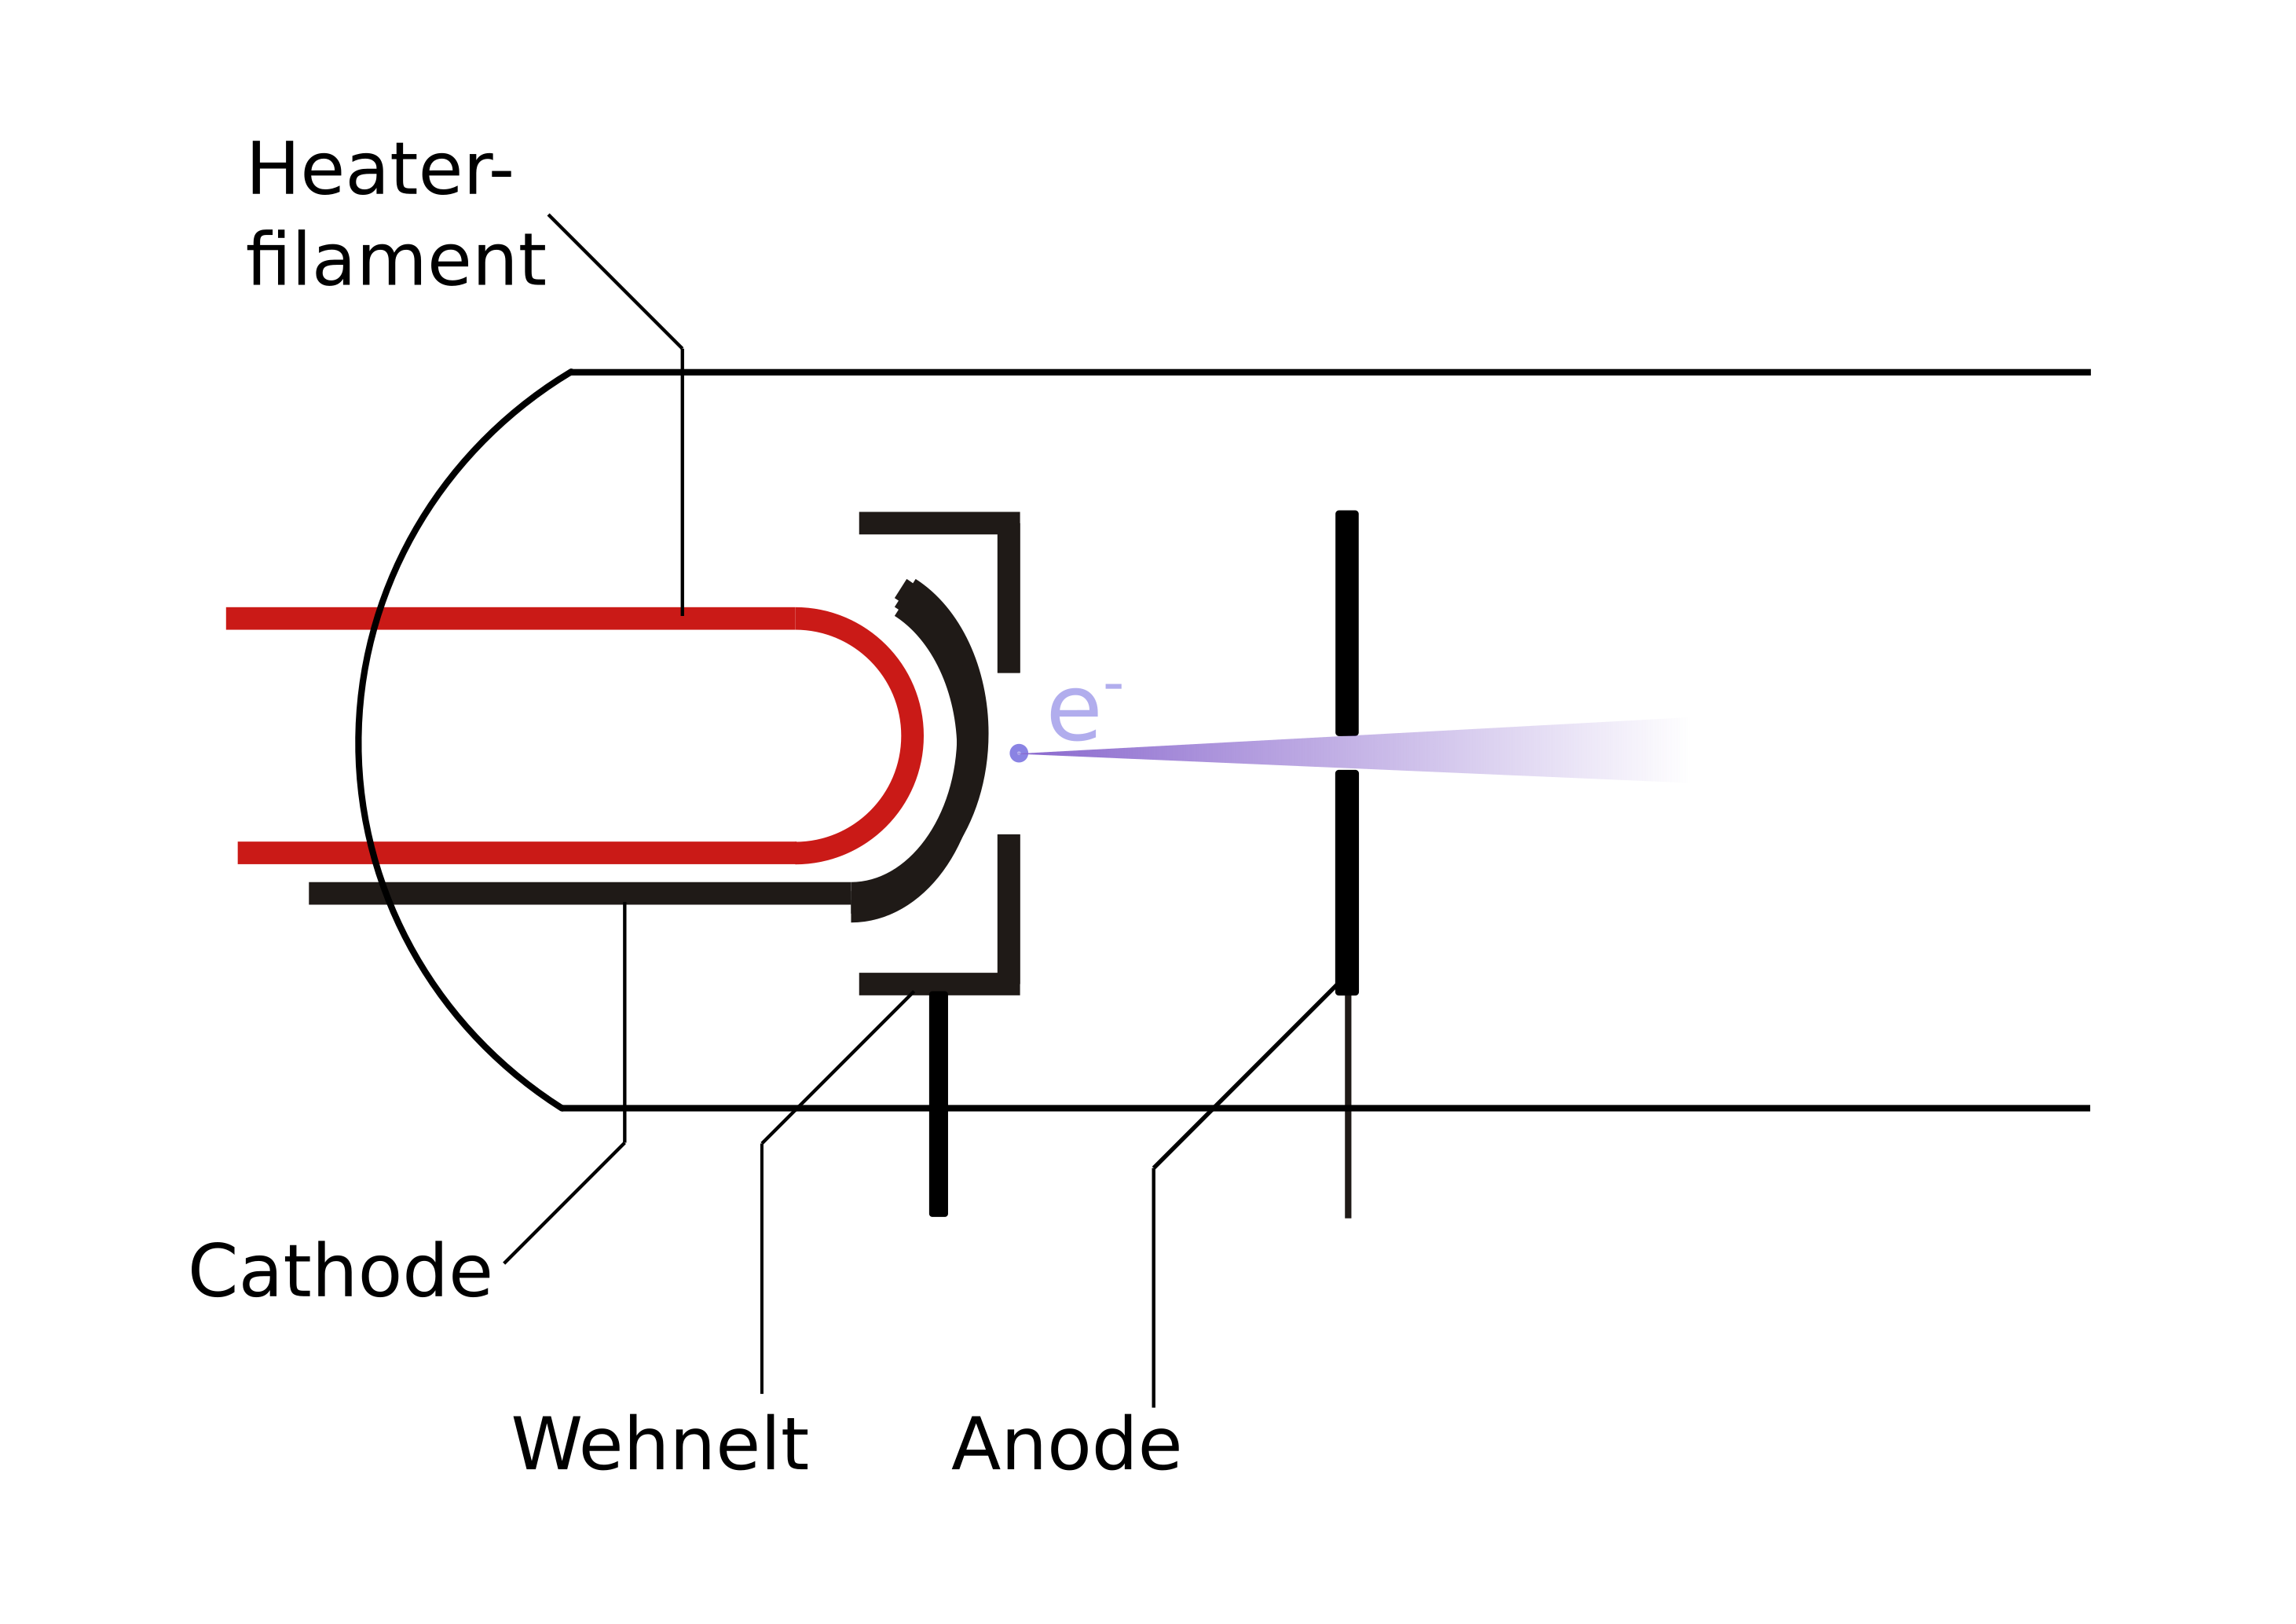
\includegraphics[width=0.9\textwidth]{Chapters/CRT-Basics/electron_gun}
	\caption{Schematic of an electron gun.}
	\label{fig:electrongun}
\end{figure}

The electron gun generates free electrons from a cathode material, accelerates them onto an anode and thereby produces an electron beam (see \cref{fig:electrongun}). One important characteristic in the selection of a cathode material is a low work function. It denotes the amount of energy needed to extract one electron from the material. There are two ways to overcome this energy barrier in an electron gun; one can either apply a strong electric field (``field emission'', ``cold cathode'')  as seen in \cref{fig:coldcathode}. Or one can heat the material until some electrons have enough thermal energy to overcome the energy barrier (``thermal emission'', ``hot cathode'', \cref{fig:hotcathode}).
In the case of the cold cathode, a cathode with a sharp tip is used, because  the electric field on the surface of a charged conductor is always strongest near sharp points. This causes the electrons to be emitted from the tip and makes for a very point-like electron source.

As our CRT uses a hot cathode, more details on this will be added later along with the description of our cathode's design.

\begin{figure}
	\centering
	\begin{subfigure}{0.4\textwidth}
		\centering
		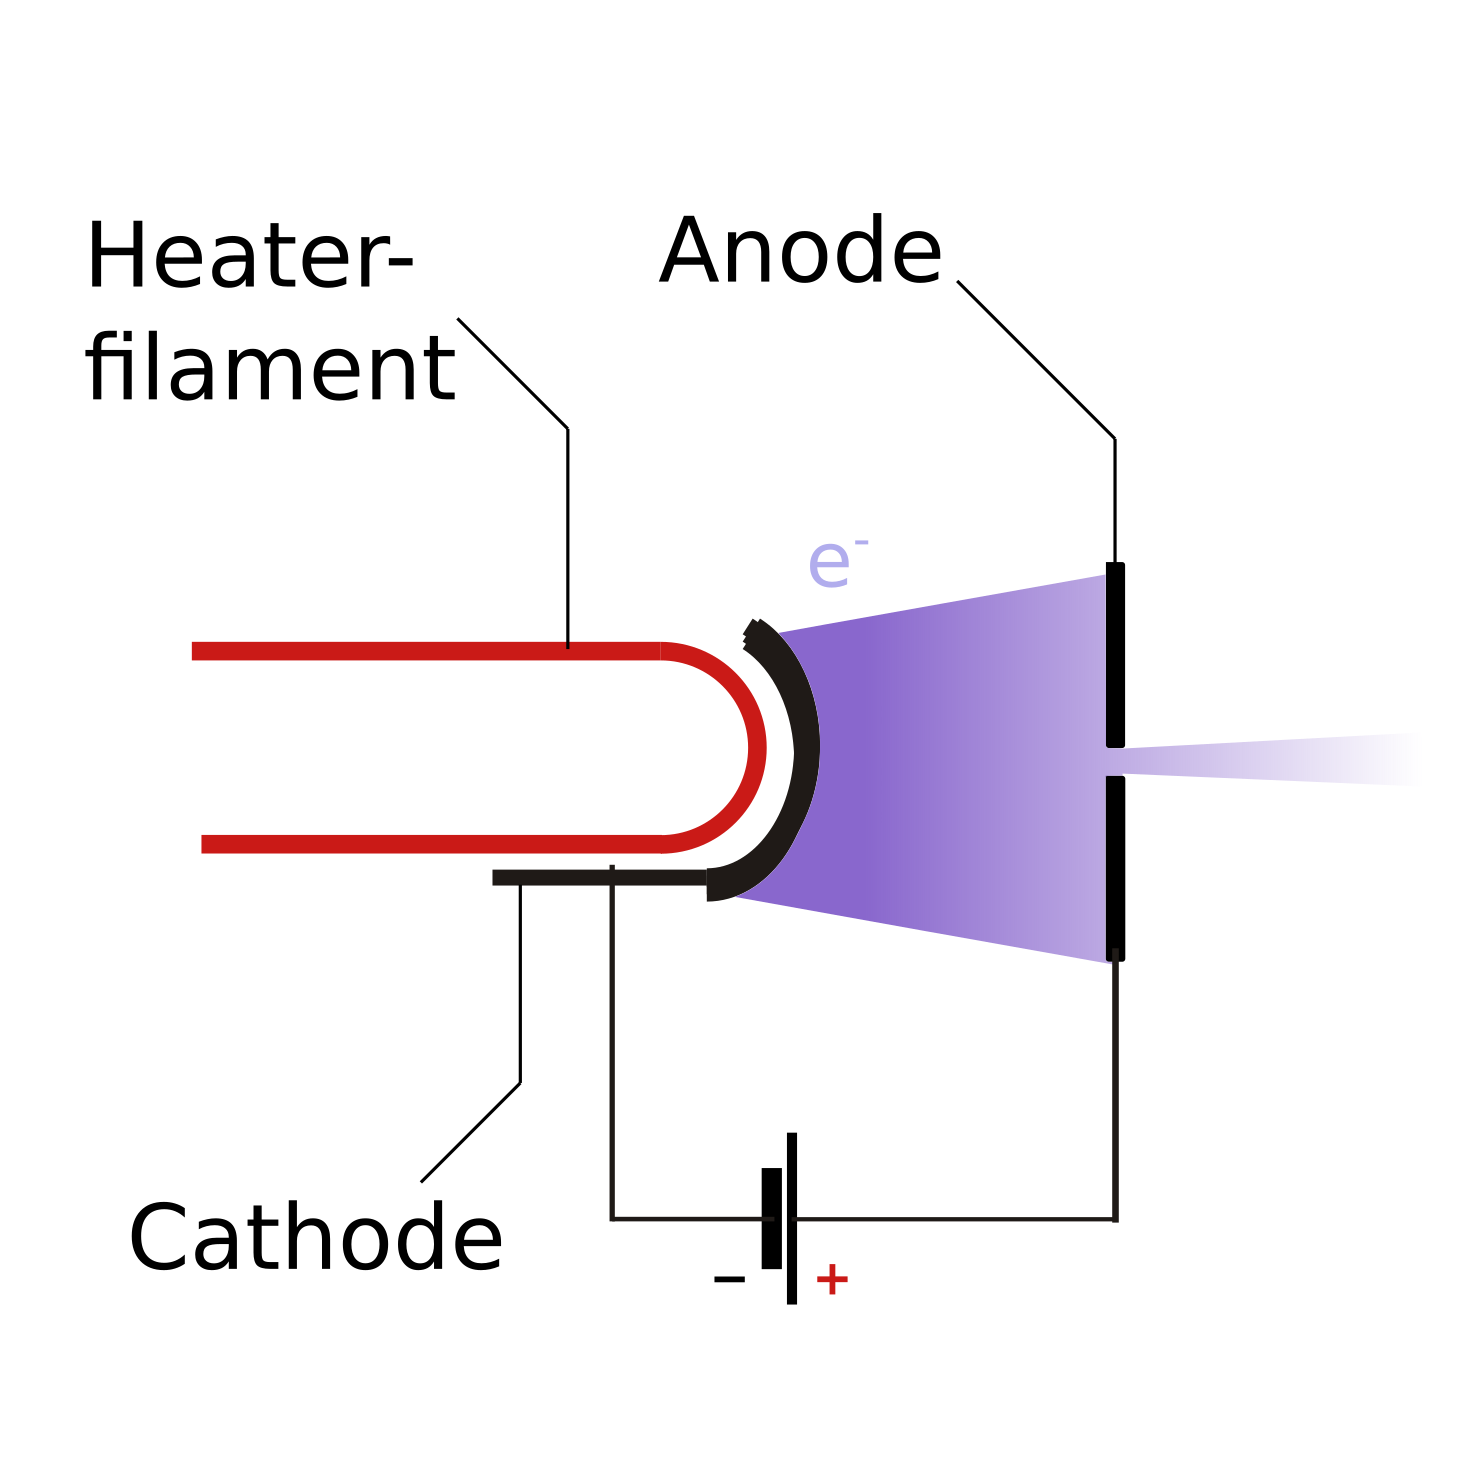
\includegraphics[width=\textwidth]{Chapters/CRT-Basics/HotCathode}
		\caption{Schematic of a hot cathode.}
		\label{fig:hotcathode}
	\end{subfigure}%
	\hspace{0.1\textwidth}
	\begin{subfigure}{0.4\textwidth}
		\centering
		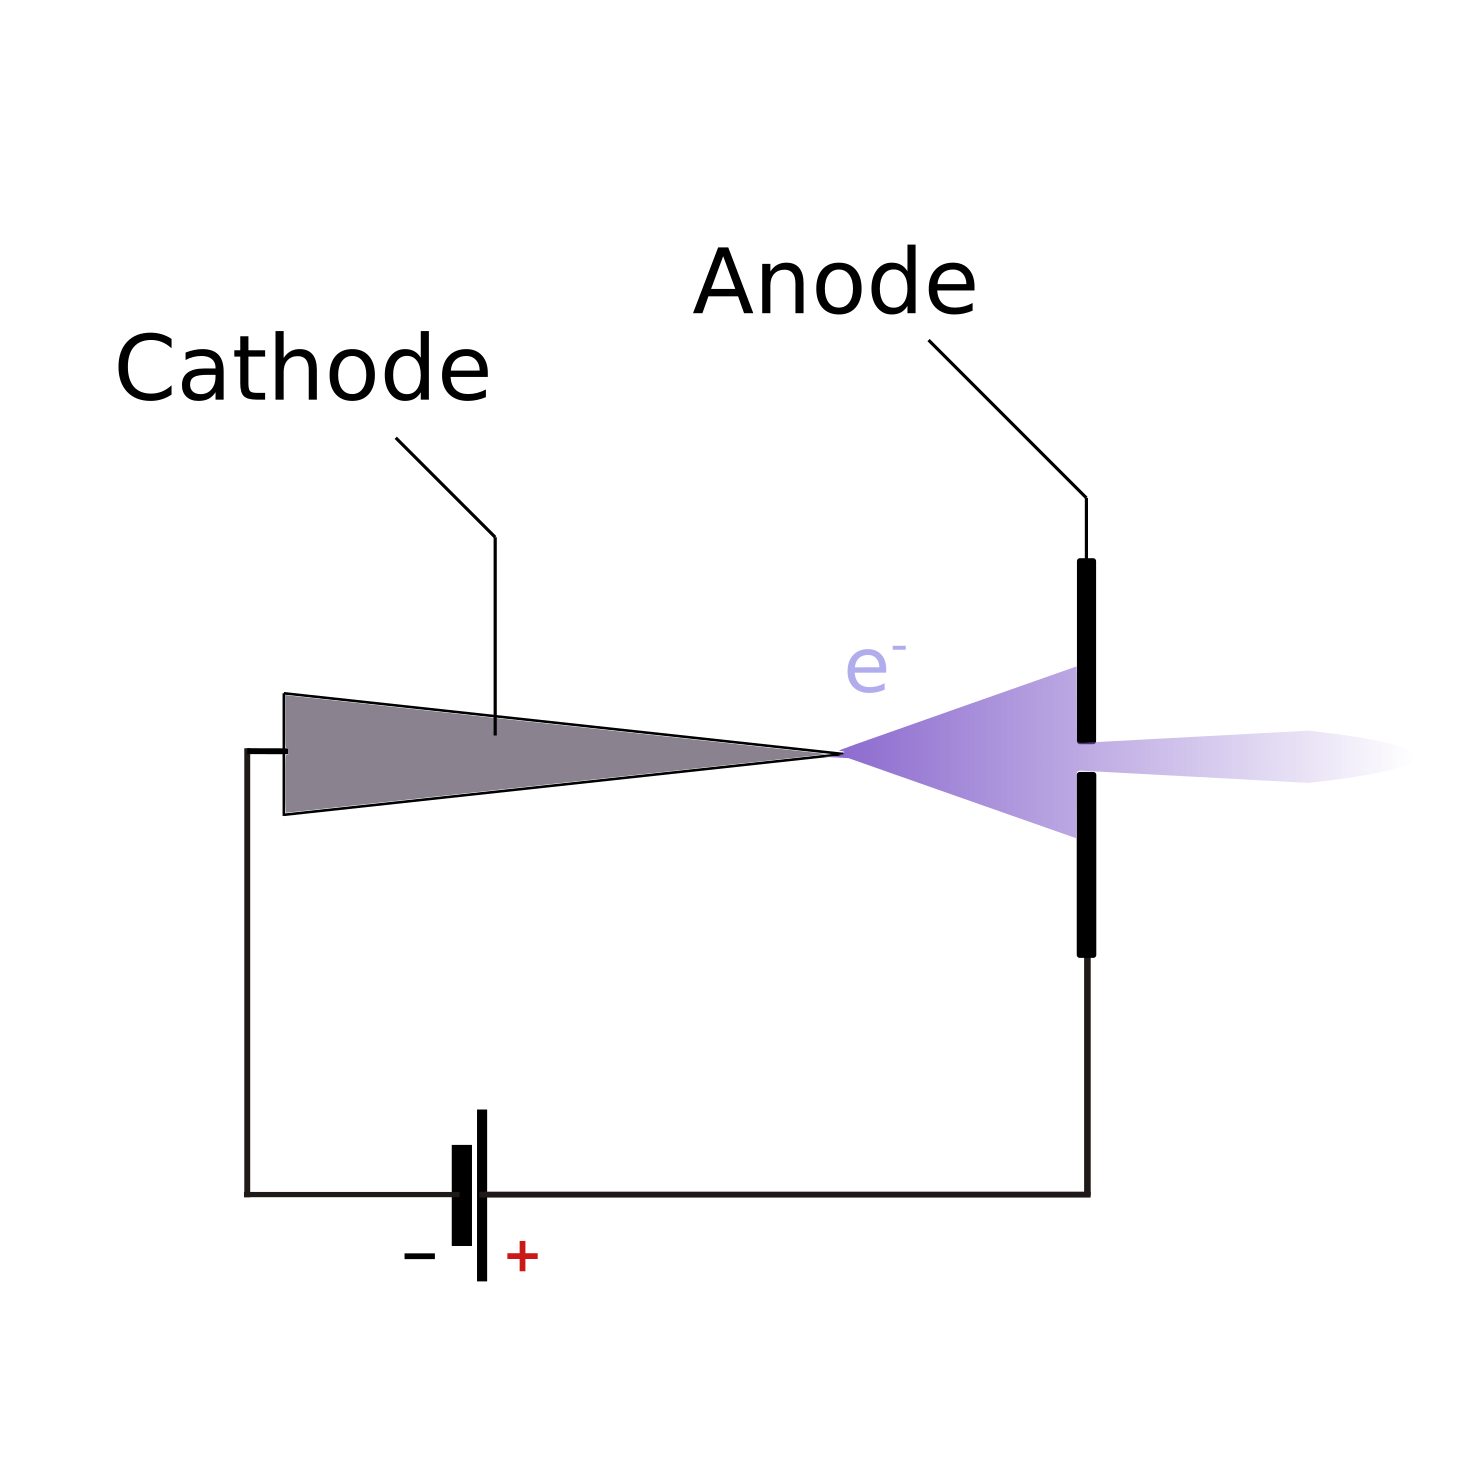
\includegraphics[width=\textwidth]{Chapters/CRT-Basics/ColdCathode}
		
		\caption{Schematic of field emission cathode.}
		\label{fig:coldcathode}
	\end{subfigure}
	\caption{Cathode types}
	\label{fig:cathodes}
\end{figure}


Normally the cathode itself is covered in beam direction in a so-called Wehnelt cylinder. Which is a conducting cylinder set to a slightly more negative potential than the cathode. This part implements two features; firstly, it condenses the emitted electrons, leading to a smaller spot size, i.e. making the cathode a more point-like electron source. Secondly, it enables us to regulate the beam current, the more negative the Wehnelt potential is, the less electrons are emitted by the electron gun. As we make the Wehnelt potential more positive, the beam current increases and continues to rise even after it is more positive than the cathode itself. However, the spot size gets increased, while the proper beam focus is lost. 

The electrons that leave the electron gun are still divergent and need to be focused. For our electrons with an energy of \SI{2}{\kilo\electronvolt},  an electrostatic lens is used.  In the simplest way these are cylindrically symmetrical pieces of conductor, like a ring or tube, set to an electrical potential. By combining several of them, one can create the same effect as a combination of concave and convex lenses \cite{Demtroeder3}. 

The field of this system is simply governed by Laplace's equation in 
cylindrical coordinates:
\begin{equation}
	0=\dfrac{1}{r}\pdv{\phi}{r}+\pdv[2]{\phi}{r}+\pdv[2]{\phi}{z}
\end{equation}

If we take the axis of the beam to be the $z$-axis, the focal point position in the $x$-$y$-plane can be shifted using the two pairs of deflection plates, one for the $x$- and one for the $y$-direction. The deflection is achieved by applying a voltage between the two parallel plates (see: \cref{fig:deflectionplate2}). By starting with an electron with kinetic energy $e \cdot U_0$ which is accelerated in $x$-direction by a constant force $e\cdot U_x / d$ over the extent of the plates $L$, the deflection angle is approximately \cite{Demtroeder3}:

\begin{equation}\label{key}
	\delta \approx \tan(\delta) \approx \frac{U_x\cdot L}{2 U_0 \cdot d}
\end{equation}

%Ende erster Abschnitt

For the measures of our CRT ($ L \approx \SI{5}{\centi\meter}$, $d \approx \SI{5}{\milli\meter}$, $U_0 \approx \SI{2}{\kilo\volt}$ and distance to screen $\approx \SI{20}{\centi\meter}$) this amounts to a deflection coefficient of around \SI{20}{\volt\per\centi\meter}, which is quite consistent with the value given in the CRT's manual.

\begin{figure}
	\centering
	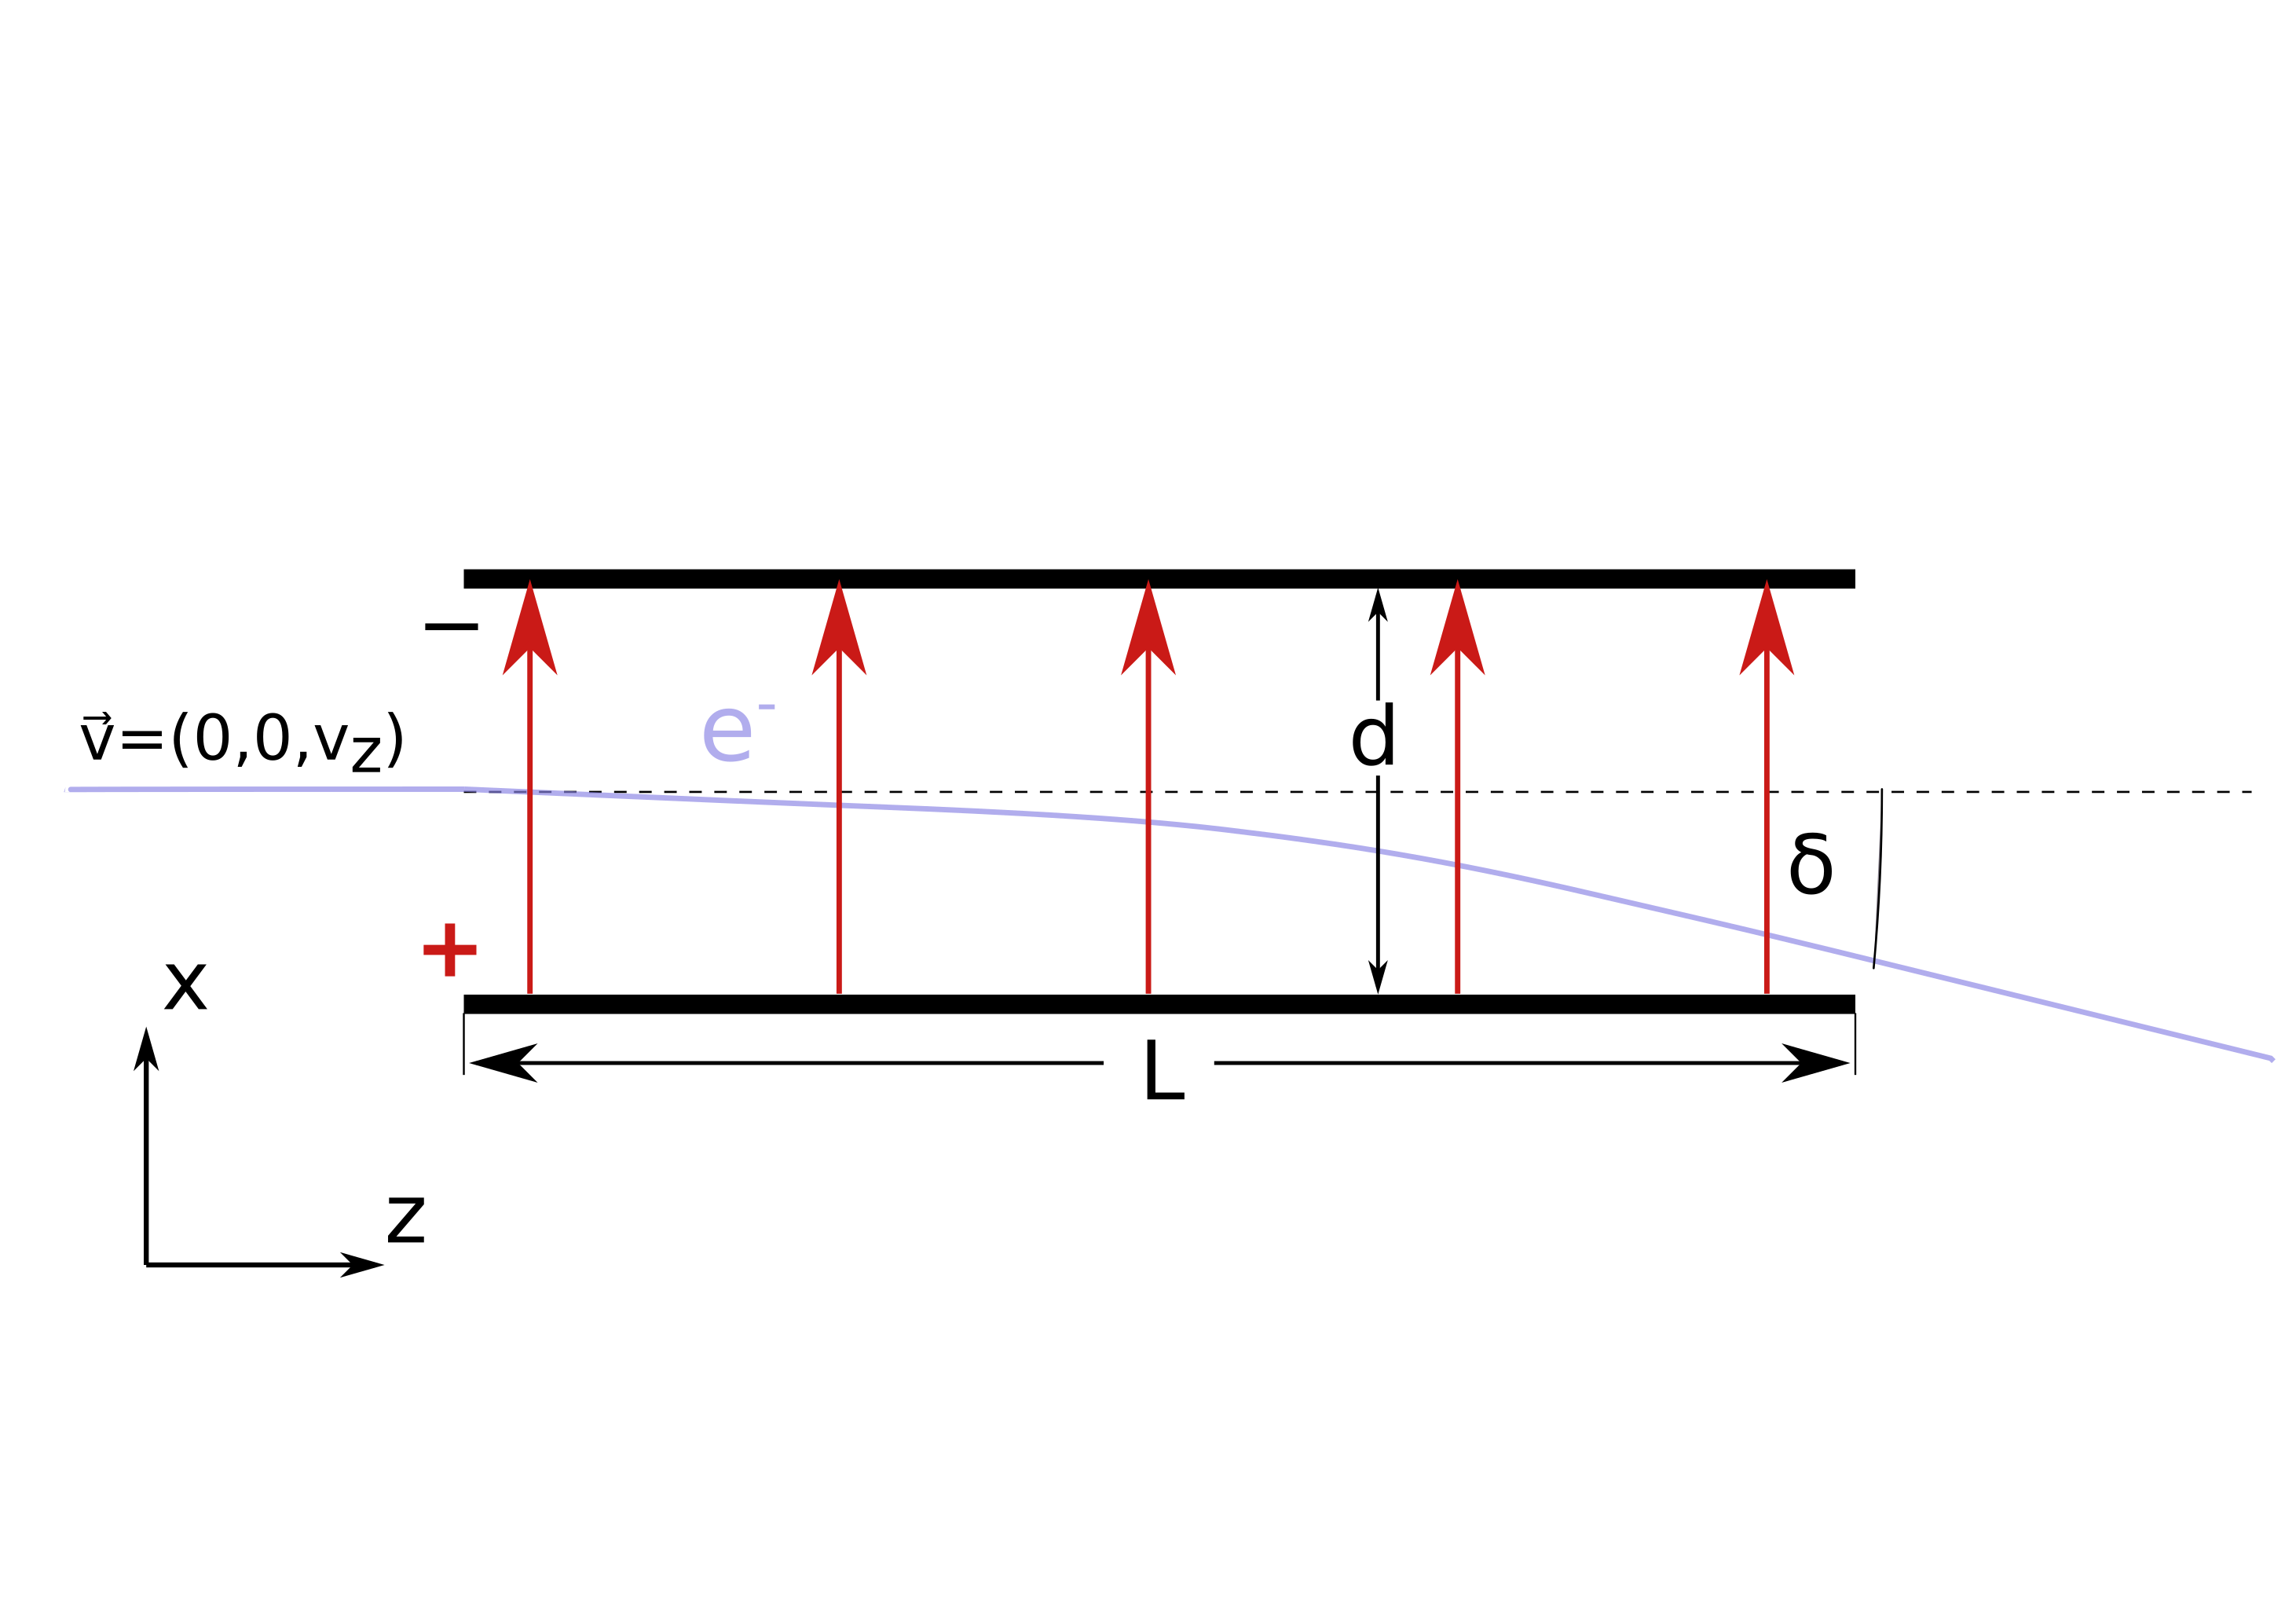
\includegraphics[width=0.7\textwidth]{Chapters/CRT-Basics/DeflectionPlate2}
	\caption{Deflection of an electron beam in a constant electrical field.}
	\label{fig:deflectionplate2}
\end{figure}

\section{Implementation in the Heerlen D14-363GY }


This section describes the CRT that is used in this project: PDS/CRT Heerlen D14-363GY. \Cref{fig:FotoCRT} shows an image of said CRT and \cref{fig:SchemeCRT} shows a schematic depiction. The cathode is not visible, as it is fixed inside the Wehnelt cylinder (1), just a few millimeters from the exit of the Wehnelt cylinder the electrons pass through the hole in the anode (2), they gain their full kinetic energy over this short distance. The electrons that go through the hole and enter the electrostatic lens, have \SI{2}{\kilo\electronvolt} and therefore move at a speed of approximately \SI{0.08}{\clight}. 
The electrostatic lenses are realized using three conducting rings (3), that are set to the same potential but have varying radii: Each consecutive ring has a smaller radius than the previous one. 

\begin{figure}
	\centering
	\begin{subfigure}{.5\textwidth}
		\centering
		\includegraphics[width=.9\textwidth]{Chapters/CRT-Basics/CRT.JPG}
		\caption{Image picture of the Heerlen D14-363GY}
		\label{fig:FotoCRT}
	\end{subfigure}%
	\begin{subfigure}{.5\textwidth}
		\centering
		\includegraphics[width=.9\textwidth]{"Chapters/CRT-Basics/electrode configuration".png}
		\caption{Schematic of the CRT from \cite{D14363GY123-manual}}
		\label{fig:SchemeCRT}
	\end{subfigure}
	\caption{}
	\label{}
\end{figure}


Between the electrostatic lens and the deflection plates, there is another aperture (4), which is internally connected to the anode and is thereby kept at the same potential. In our Setup, the deflection plates are not simply parallel but are shaped like funnels (5,7), between the two pairs of deflection plates, we have the final aperture (6). Its potential can be regulated separately (usually it's on the same potential as the anode) 


Finally the beam hits the phosphorous-coated screen which fluoresces on electron impact.

It is connected to the aquadag \footnote{A conductive coating used in CRTs, it consists of graphite particles dispersed in water.} coating inside the glass envelope and prevents charge building up that could lead to image distortions. 
Finally, the beam hits the phosphorous-coated screen, which fluoresces on electron impact.

\subsection{The Cathode}


As already mentioned, we are using a hot cathode, where electrons are thermally exited  to leave the material. Compared to cold cathodes which work by field emission, this leads to a broader energy distribution. For electron microscopy, where a high resolution is the goal, this in undesirable, as it leads to some degree of chromatic aberration in the electron optics; for our purposes this should not be a problem. On the other hand, hot cathodes normally allow for higher current densities. This is very important to QUAK because a high current density allows for a high amplitude of the beam's dipole radiation and therefore a strong coupling to the potassium atoms. The  electron current by thermal emission is described by \cite[chp 3.2.3]{Whitaker}:

\begin{equation}\label{eq:thermionic_current}
I=A\cdot T^2 \cdot e^{-b/T}
\end{equation}

Where $b$ is proportional to the work function of the material, $T$ is temperature and $A$ is a material-dependent constant. It is clear from this formula, that a low work function and a high melting point are important characteristics for a good cathode material. 

The cathode from one of our Heerlen D14-363GY-tubes has been removed and examined with EDX (Energy-dispersive X-ray Spectroscopy). Nickel, barium, and strontium have been found, which suggests that it is a metal oxide cathode with barium-, strontium-, and possibly aluminum-oxide. This type of cathode is very common in low power electron tubes.

\begin{figure}
	\centering
	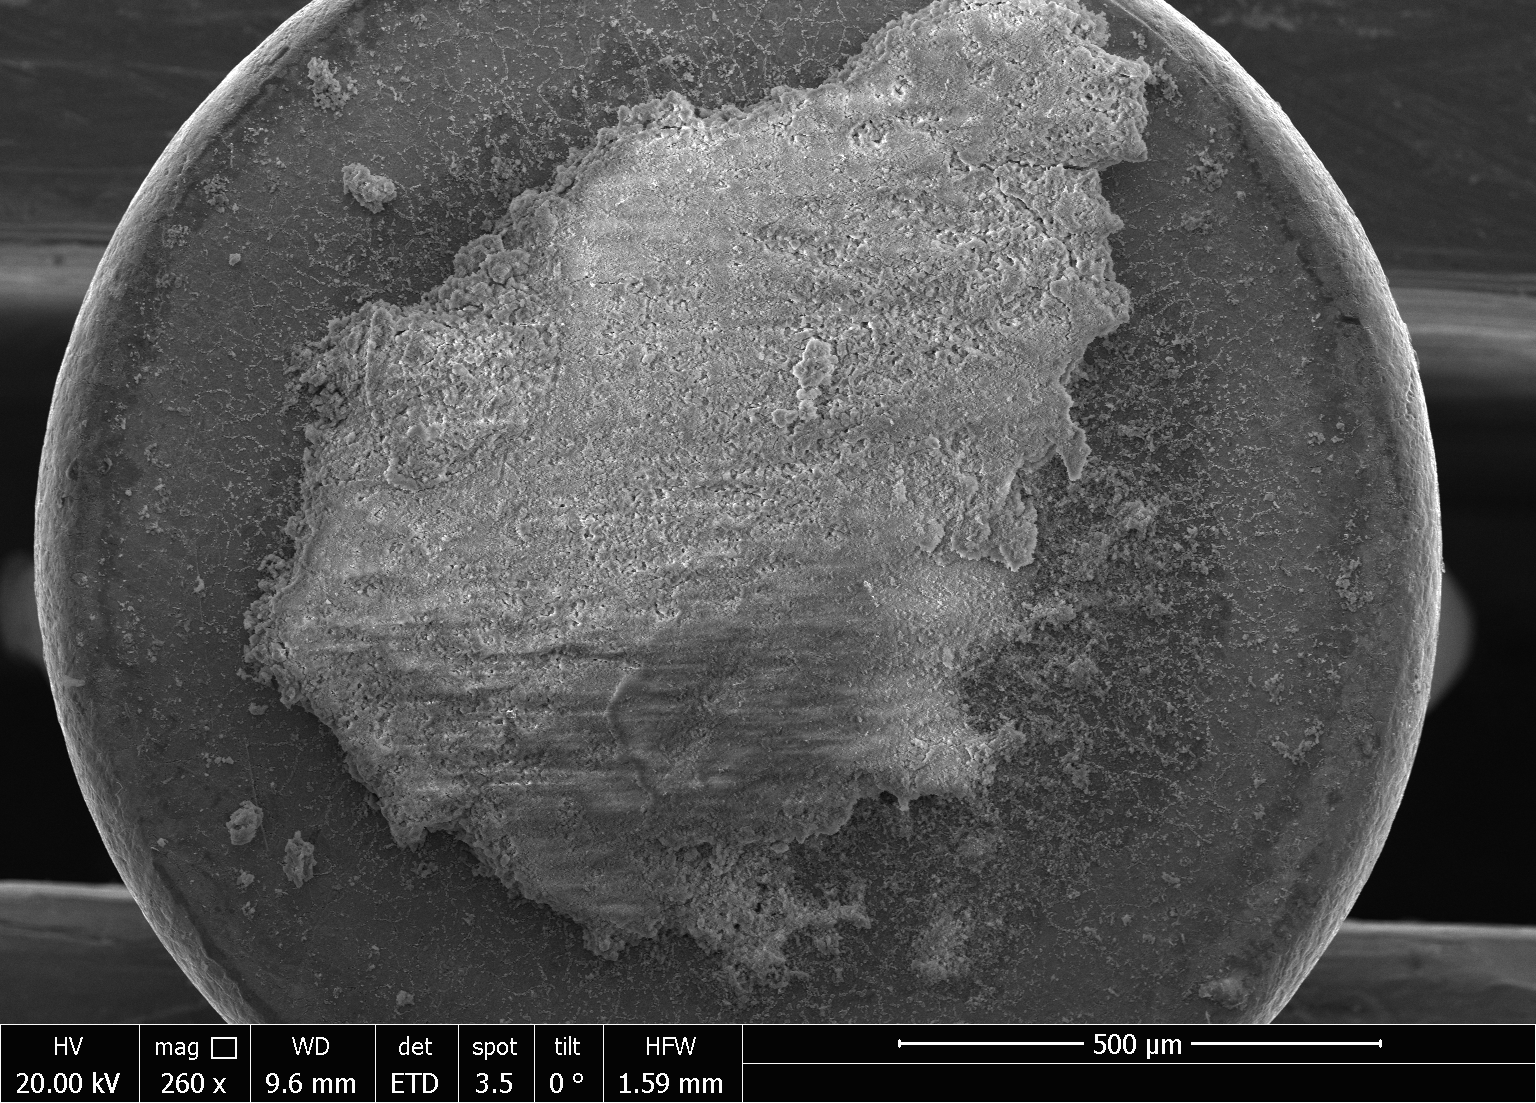
\includegraphics[width=0.7\textwidth]{Chapters/CRT-Basics/SEM_image.png}
	\caption{SAM image of metal oxide cathode.}
	\label{fig:SEM_Cathode}
\end{figure}

The ``Power Vacuum Tubes Handbook'' \cite[chp 3.5.2.1]{Whitaker} describes a typical oxide cathode as a coating of barium and strontium oxides on a structure made from nickel alloys. Nickel is chosen for its strength and toughness, which it retains even at high temperatures. These cathodes are normally made by coating a case structure with a mixture of barium and strontium carbonates (typically \SI{60}{\percent} Ba and \SI{40}{\percent} Sr), suspended in a binder material and then baking the structure, causing the carbonates to be reduced to oxides. 

These metal oxide cathodes normally operate at \SIrange{700}{820}{\celsius} and are capable of average emission densities of \SIrange{100}{500}{\milli\ampere\per\centi\meter\squared}. Higher peak emissions are possible for shorter periods of time. As already mentioned, one of the advantages of this type of cathode is its high emission current capability compared to cathodes made from other materials. Downsides to this cathode type are its greater susceptibility to so-called oxygen poisoning and to ion bombardment. The literature therefore recommends to avoid prolonged exposure to oxygen. Oxygen poisoning is the process in which oxygen adsorbs onto the cathode and increases its work function, effectively reducing the ability to emit electrons. 


Also the material from the oxide cathode will evaporate during the tube's lifetime and will travel to other parts of the tube, adsorbing to electron optics parts and turning them into additional emitters. The literature (\cite[chp 3.5.2.1]{Whitaker}) therefore, also advises against exceeding the design value for the heater voltage, as this reduces the lifetime of the cathode significantly. CRTs are typically designed to operate for ten years or longer. For QUAK however, a shorter lifetime is acceptable. Therefore during the course of our project, we did drive the cathode with higher heater voltages on various occasions in order to increase the available beam current. We still don't know exactly how fast the degradation due to this effect proceeds; further research is necessary.  

\subsection{Cathode Layout}

\Cref{fig:cathodelayout} shows how metal oxide cathodes for CRTs typically look. The depiction agrees very well with the layout of our cathode. On the image we see the cathode cylinder, which corresponds to the nickel support structure mentioned above. It is shaped into a cup, in which the heater filament (shaped into a coil) is inserted. The oxide disk, from where the electrons are emitted, is baked onto the top of the cathode cylinder. The cathode cylinder is mounted on an isolating support structure and inserted into the Wehnelt cylinder, which is called ``grid cup'' in the drawing. 
  

\begin{figure}
	\centering
	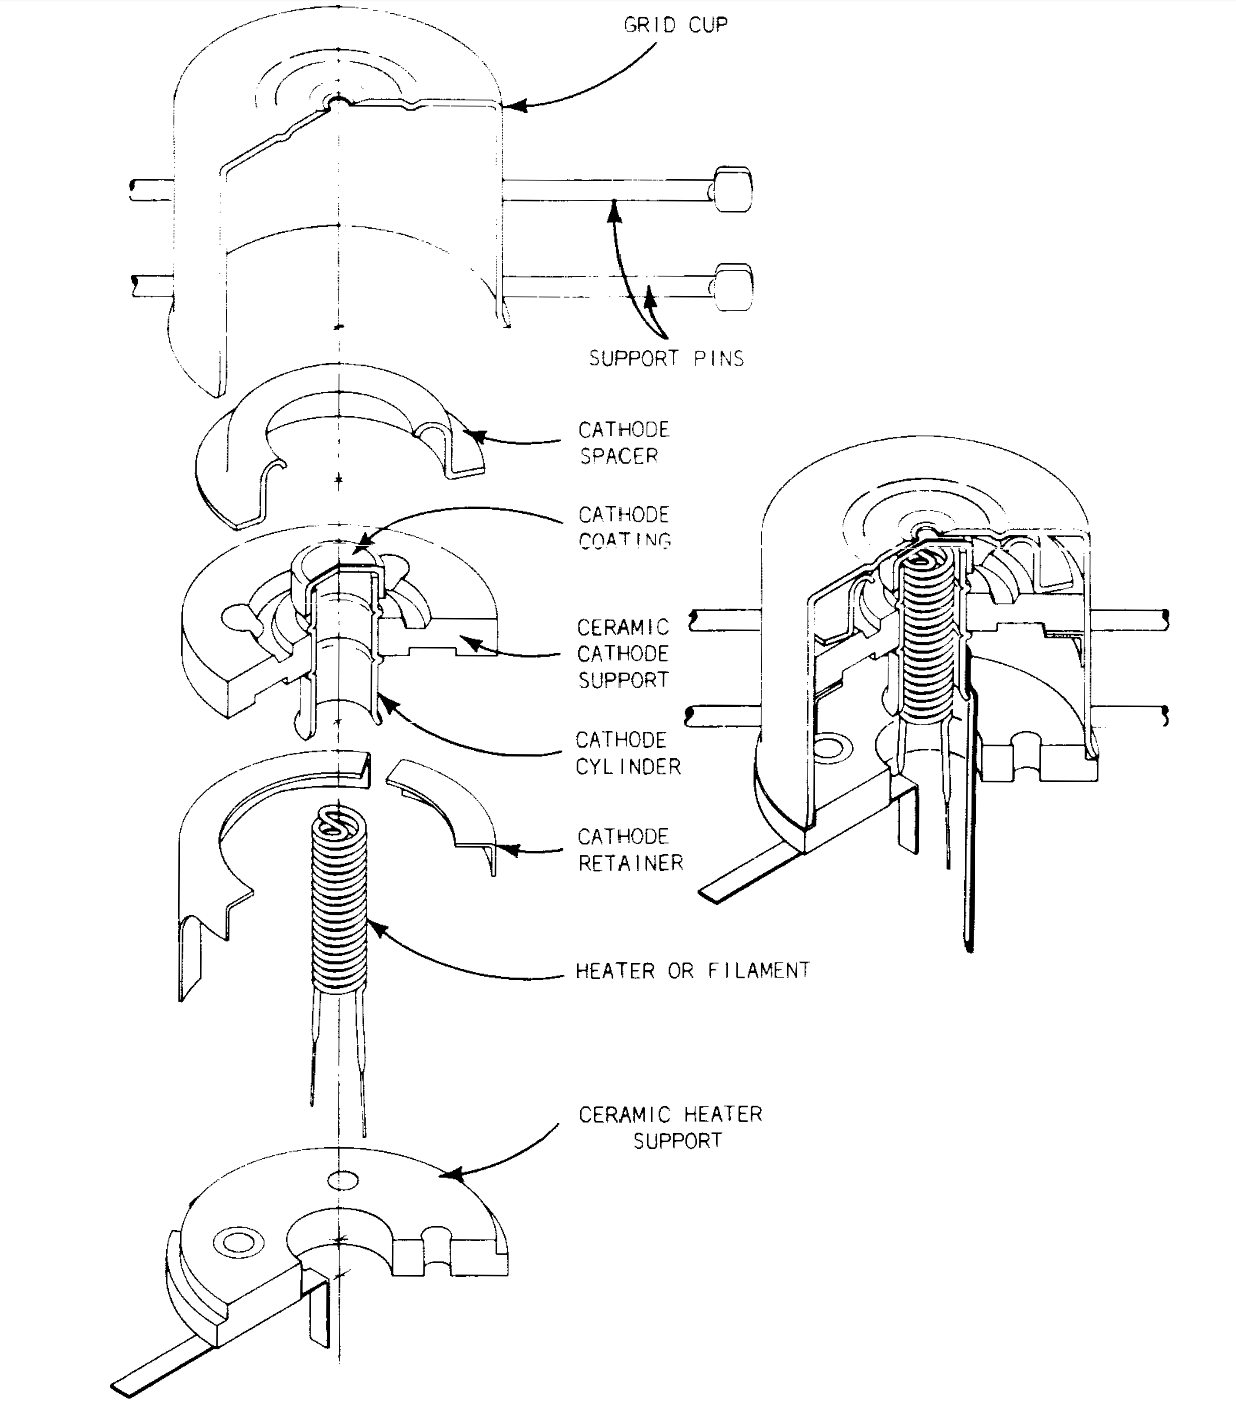
\includegraphics[width=0.6\textwidth]{Chapters/CRT-Basics/Cathode_layout}
	\caption{Schematic of the layout of a typical CRT-cathode \cite{deVere69}.}
	\label{fig:cathodelayout}
\end{figure}















%% !TeX encoding = UTF-8
% !TeX spellcheck = en_US
% !TeX root = ../../Thesis.tex

\chapter{Cicero Word Generator}\label{chap:Cicero, Cicero Word Generator}
This chapter describes the installation and initial setup of Cicero Word Generator\autocite{keshet2013distributed} on a PC running Windows 10 with analog and digital cards from National Instruments (NI). The code is freely available on Github\autocite{akeshet:Github}. This chapter contains only differences, problems, and possible solutions encountered when Cicero was installed for the PC `Fritz Fantom' which will be used for the QuaK experiment. It is therefore advised to use the technical and user manual\autocite{akeshet:manual} in conjunction. The titles in this chapter and font style with {\fontfamily{pcr}\selectfont Courier} and \textbf{Boldface} was mirrored to fit the manual.

\section{Installation of National Instruments drivers}\label{sec:Cicero, Installation of National Instruments drivers}
Before setting up the Cicero Word Generator, it is necessary to install the newest .NET Framework\autocite{microsoft:download.net} from Microsoft. For the first installation of NI drivers, NI-DAQmx (version 9.3), NI-VISA (newest version), and NI-4888.2 (newest version) should be downloaded from the National Instruments website\autocite{ni:drivers}. When installing the NI drivers it is possible to get an `Runtime Error!'. In this case it is necessary to set the Regional format settings of Windows 10 to `English (United States)'\autocite{ni:runtimeerror}.

\section{Installation of National Instruments Cards}\label{sec:Cicero, Installation of National Instruments Cards}
After installation of the necessary drivers, the physical cards can be inserted into the PCIe slots on the motherboard. On `Fritz Fantom' the digital card (NI PCIe-6537B) was installed in PCIe bus 3 while the analog cards (NI PCIe-6738) were installed in PCIe bus 4 and 5.

\section{Configuring Atticus}\label{sec:Cicero, Configuring Atticus}
After installation of the NI cards, Atticus should be launched for the first time and closed without changing any settings. After this, the NI-DAQmx drivers should be updated to the newest version. If version 9.3 was not used when launching Atticus in this step, it could result in an error. After this, ``Configuring Atticus'' on the user manual can be followed. The \textbf{Server Name} was set to `Fritz\_Phantom'\todo[caption={namechange?}]{change server name in lab? Fantom, not Phantom}. \textbf{Dev1} to \textbf{Dev3} were set in the same ascending order as the physical installation on the motherboard.

\subsection{Configure hardware timing / synchronization}\label{subsec:Cicero, Configure hardware timing / synchronization}
For synchronization, a \textbf{Shared Sample Clock} was used with \textbf{Dev1} being the master card. The settings are summarized in \cref{tab:settings dev1} and \cref{tab:settings dev2}. For \textbf{Dev3} `SampleClockExternalSource' should be set to `/Dev3/RTSI7'. The `SampleClockRate' is set to \SI{350}{\kilo\hertz} since this is the fastest rate with all 32 analog channels active. It is possible to raise this to \SI{1}{\mega\hertz} by only using 8 channels (1 channel per bank).
\begin{table}[H]
	\centering
	\caption{Settings for \textbf{Dev1}.}
	\label{tab:settings dev1}
	\begin{tabular}{*{2}{|l}|}
		\hline
		\textbf{Setting} & Value \\ \hline
		MasterTimebaseSource & \\ \hline
		MySampleClockSource & DerivedFromMaster \\ \hline
		SampleClockRate & 350000 \\ \hline
		UsingVariabletimebase & False \\ \hline
		SoftTriggerLast & True \\ \hline
        StartTriggerType & SoftwareTrigger \\ \hline
	\end{tabular}        	
\end{table}

\begin{table}[H]
	\centering
	\caption{Settings for \textbf{Dev2}.}
	\label{tab:settings dev2}
	\begin{tabular}{*{2}{|l}|}
		\hline
		\textbf{Setting} & Value \\ \hline
		MasterTimebaseSource & \\ \hline
		MySampleClockSource & External \\ \hline
		SampleClockExternalSource & /Dev2/RTSI7 \\ \hline
		SampleClockRate & 350000 \\ \hline
		UsingVariabletimebase & False \\ \hline
		SoftTriggerLast & False \\ \hline
		StartTriggerType & SoftwareTrigger \\ \hline
	\end{tabular}        	
\end{table}

\section{Configuration and Basic Usage of Cicero}\label{sec:Cicero, Configuration and Basic Usage of Cicero}
After setting up the Atticus server, Cicero can be configured. In step 3.c. it is necessary to write the full IP address and not `localhost'. Once step 6 is finished, Cicero should run without any problems.

\section{Saving of Settings and Sequences}\label{sec:Cicero, Saving of Settings and Sequences}
The `SettingsData' of the Server Atticus are saved in C:\textbackslash Users\textbackslash confetti\textbackslash Documents \textbackslash Cicero\textunderscore Atticus\textbackslash Cicero\textbackslash SettingsData while the `SequenceData' of Cicero are saved in C:\textbackslash Users\textbackslash confetti\textbackslash Documents\textbackslash Cicero\textunderscore Atticus\textbackslash Cicero\textbackslash SequenceData.

\section{Sequence length limit}\label{sec:cicero, Sequence length limit}
The duration of a sequence is limited to $\num[exponent-base=2]{e32}/(16*32*\SI{350}{\kilo\hertz})$ = \SI{23.967}{\second} coming from a 32-bit application, \SI{16}{\bit} per channel, 32 channels in a NI PCIe-6738 card, and \SI{350}{\kilo\hertz} clock rate.
%% !TeX encoding = UTF-8
% !TeX spellcheck = en_US
% !TeX root = ../../Thesis.tex
\chapter{Electron beam setup}
\label{ch:Electron beam setup}

\section{Charatarization of a working CRT}
\label{sec:Charatarization of a working CRT}

HAMEG HM507 oscilloscopes \autocite{HM507-manual} were used for testing purposes. These contain a D14-363GY/123 \autocite{D14363GY123-manual} CRT. Although it only has a bandwidth of \SIrange{0}{50}{\mega\hertz}, which is not sufficient to reach the hyperfine splitting frequency of \SI{461.7}{\mega\hertz} for $^{39}\mathrm{K}$ \cite{tiecke:potassium-properties} (or \SI{254}{\mega\hertz} for $^{41}\mathrm{K}$), it was used nevertheless because of its simple construction and availability. The back pin arrangement is shown in \cref{fig:pin arrangement}.

The voltages and currents of the pins to drive the CRT were measured using a \SI{2.5}{\kilo\volt} probe with a voltage divider of 100:1 and are summarized in \cref{tab:D14-363GY/123 tube pin measurements}. It was not possible to measure pin g3 directly. Therefore a HVPS (\cref{sec:HVPS}) was used to set a voltage and the beam diameter was observed. The best focus was achieved with the value written in the table. The voltage offset of x-, and y-plates was not possible to measure directly, since it varies with time to draw the necessary image on the phosphor screen. The given values are the mean of the minimum and maximum measured voltage. The deflection coefficient is summarized in \cref{tab:D14-363GY/123 deflection coefficient}.

\begin{figure}[ht]
	\centering
	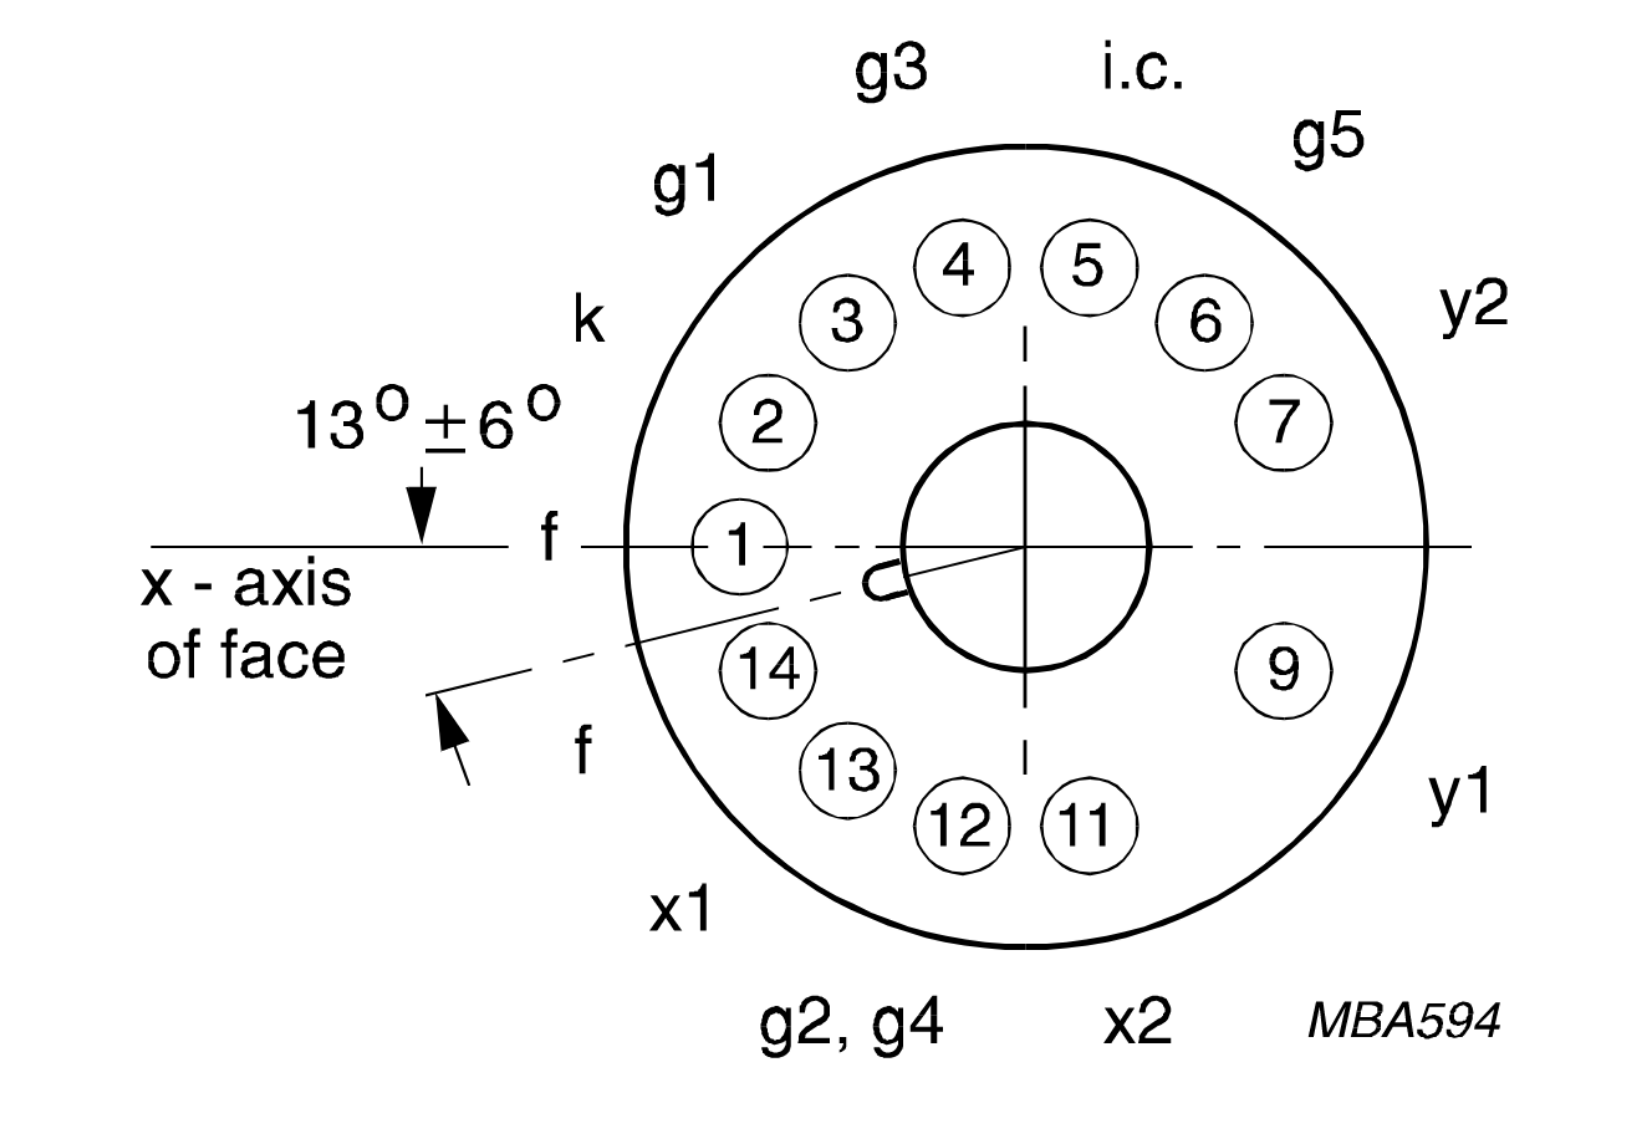
\includegraphics[width=5cm]{./Chapters/e-beam-setup/pin arrangement}
	\caption{Pin arrangement, bottom view \autocite{D14363GY123-manual}.}
	\label{fig:pin arrangement}
\end{figure}


\begin{table}[ht]
	\centering
	\caption{D14-363GY/123 CRT pin measurements.}
	\label{tab:D14-363GY/123 tube pin measurements}
	\begin{tabular}{S r *{2}{S}}
		\toprule
		{number} & pin    & {voltage/\si{\volt}} & {current/\si{\micro\ampere}} \\
		\midrule
		1      & f      & -1.99e3              & 86.6e3 \\
		2      & k      & -2.00e3              & -7.6 \\
		3      & g1     & -2.03e3              & 0 \\
		4      & g3     & -1.813e3             & 0 \\
		5      & i.c.   & 71.7                 & 0.1 \\
		6      & g5     & 64.                  & 7.2 \\
		7      & y2     & 78                   & {-} \\
		9      & y1     & 78                   & {-} \\
		11     & x2     & 96                   & {-} \\
		12     & g2, g4 & 71.0                 & 0 \\
		13     & x1     & 96                   & {-} \\
		14     & f      & -1.97e3              & -86.2e3 \\
		\bottomrule
	\end{tabular}
\end{table}

\begin{table}[ht]
	\centering
	\caption{D14-363GY/123 deflection coefficients \autocite{D14363GY123-manual}.}
	\label{tab:D14-363GY/123 deflection coefficient}
	
	\begin{tabular}{*{2}{l} l}
		\toprule
		horizontal & $M_x$ & \SI{19}{\volt/\centi\meter} \\
		vertical   & $M_y$ & \SI{11.5}{\volt/\centi\meter} \\
		\bottomrule
	\end{tabular}
\end{table}


\section{High Voltage Power Supply HVPS}
\label{sec:HVPS}

To produce high dc voltages to drive the CRT, four HCP 14-6500 power supplies \autocite{fug-hcp-manual} were used. They were named `HVPS 1' to `HVPS 4' and can provide up to \SI{2}{\milli\ampere} at \SI{\pm 6.5}{\kilo\volt}. To connect the output to the CRT pins, BNC cables were refitted with a save high voltage (SHV) connector on one side while on the other end the BNC connector was kept (\cref{fig:Coaxial cable with SHV and BNC connector}). A \SI{6}{\kilo\volt} probe was used to obtain the breakdown voltage, which is around \SI{3}{\kilo\volt} caused by the coaxial cable which was not built do sustain high voltages.

\begin{figure}[ht]
	\centering
	
	\includegraphics[width=.9\textwidth]{"Chapters/e-beam-setup/SHV.JPG"}
	%\missingfigure[figwidth=0.9\textwidth]{Figure of SHV \& BNC connector cable.}
	
	\caption{Coaxial cable with SHV and BNC connector.}
	\label{fig:Coaxial cable with SHV and BNC connector}
	\todo[inline]{annotate BNC and SHV}
\end{figure}

\subsection{Ripple measurement}
\label{subsec:ripple measurement}
Each power supply was measured for its ripple with a set voltage of \SI{2}{\kilo\volt}. A \SI{2.5}{\kilo\volt} probe (attenuation ratio 100:1) was connected to an oscilloscope set to ac coupling with a timescale of \SI{1}{\milli\second}. To get the electronic noise of the oscilloscope itself, the probe was shorted and the noise measured. A picture of a measurement is shown in \cref{fig:measurement HVPS ripple} with the values summarized in \cref{tab:measurement HVPS ripple}. As can be seen, the ripple is very close to the noise level and can not really be distinguished.

\begin{figure}[ht]
	\centering
	
	\includegraphics[width=0.9\textwidth]{./Chapters/e-beam-setup/ripple HVPS1}

	\caption{Measurement of HVPS ripple.}
	\label{fig:measurement HVPS ripple}
\end{figure}

\begin{table}[ht]
	\centering
	\caption{HVPS ripple}
	\label{tab:measurement HVPS ripple}
	\begin{tabular}{l S}
		\toprule
		device & {ripple/\si{\milli\volt}} \\
		\midrule
		short  & 116 \\
		HVPS 1 & 136 \\
		HVPS 2 & 138 \\
		HVPS 3 & 194 \\
		HVPS 4 & 204 \\
		\bottomrule
	\end{tabular}
\end{table}

\section{CRT wiring}\label{sec:CRT wiring}
A schematic of the supplied power is shown in \cref{fig:schematics of wiring}. The pin i.c. stands for internally connected and is wired to pin g2, g4. A small ac or dc voltage is necessary to drive the heater filament f. This part of the setup is explained in \cref{sec:Heater}.


\begin{figure}[H]
	\centering
	
	\begin{circuitikz}[european]
		% !TeX encoding = UTF-8
% !TeX spellcheck = en_US
% !TeX root = ../../Thesis.tex


%\draw [help lines] (0,0) grid (10,10);
		
\newcommand{\hvps}[2] % corordinates of bottom left corner, label
% draw a hvps
{		
	% draw HVPS
	\draw (0 + {#1}[0], 0 + {#1}[1]) rectangle (2.5 + {#1}[0], 2.5 + {#1}[1]); % box of size 2.5
	\node[above] at (1.25 + {#1}[0], 2.5 + {#1}[1]) {#2};	% label for box
	\draw (3 + {#1}[0], 1 + {#1}[1]) -- (1.5 + {#1}[0], 1 + {#1}[1]) to[vsource] (1.5 + {#1}[0], 2 + {#1}[1]) -- (3 + {#1}[0], 2 + {#1}[1]);  % voltage supply
	\draw (1.5 + {#1}[0], 0.5 + {#1}[1]) -- (3 + {#1}[0], 0.5 + {#1}[1]) node[ground] {}; % ground
}

\newcommand{\coaxial}[2] % coordinates of left inner wire, length of cable
% draw a coaxial cable with given length
{
	\draw (0 + {#1}[0], {#1}[1]) to[short, *-*] (#2 + {#1}[0], {#1}[1]); % middle line
	\draw (1 + {#1}[0], {#1}[1]) circle [radius=0.5]; % left circle
	\draw (#2 - 1 + {#1}[0], {#1}[1]) circle [radius=0.5]; % right circle
	\draw (1 + {#1}[0], 0.5 + {#1}[1]) -- (#2 - 1 + {#1}[0], 0.5 + {#1}[1]); % top line
	\draw (0 + {#1}[0], -0.5 + {#1}[1]) to[short, *-*] (#2 + {#1}[0], -0.5 + {#1}[1]); % bottom line
}

% HVPS 4
\hvps{(0, 0)}{HVPS 4}
\draw (3, 2) -- (3, 1.5);
\coaxial{(3, 1.5)}{5}
\draw (8, 1.5) -- (10, 1.5);
\node [right] at (10, 1.5) {i.c.};

% HVPS 3
\hvps{(0, 4)}{HVPS 3}
\draw (3, 6) -- (3, 5.5);
\coaxial{(3, 5.5)}{5}
\draw (8, 5.5) -- (10, 5.5);
\node [right] at (10, 5.5) {g3};

% HVPS 2
\hvps{(0, 8)}{HVPS 2}
\draw (3, 10) -- (3, 9.5);
\coaxial{(3, 9.5)}{5}
\draw (8, 9.5) -- (10, 9.5);
\node [right] at (10, 9.5) {f};
\draw (9, 9.5) to[sV, *-] (9, 8); % ac voltage source
\draw (9, 8) to[short, *-] (10, 8);
\node [right] at (10, 8) {f};
\draw (9, 8) -- (9, 7) -- (10, 7);
\node [right] at (10, 7) {k};

% HVPS 1
\hvps{(0, 12)}{HVPS 1}
\draw (3, 14) -- (3, 13.5);
\coaxial{(3, 13.5)}{5}
\draw (8, 13.5) -- (10, 13.5);
\node [right] at (10, 13.5) {g1};
	\end{circuitikz}

	\caption{Schematics of supplying CRT pins with power.}
	\label{fig:schematics of wiring}
\end{figure}


\section{Heater}
\label{sec:Heater}

\begin{figure}[ht]
	\centering
	
	\begin{subfigure}[b]{0.9\textwidth}
		\begin{circuitikz}%[width=0.9\textwidth]
			% !TeX encoding = UTF-8
% !TeX spellcheck = en_US
% !TeX root = ../../Thesis.tex


%\draw [help lines] (0, 0) grid (8, 4);
%\filldraw (0, 0) circle (0.5mm);

% left half with transformer
\draw (0, 0)
to [sV, label = \SI{230}{\volt}] ++ (0, 2)
to [normal open switch]  ++ (2, 0);
\draw (2, 2) node [transformer core, anchor=A1] (transformer) {}
	(transformer.inner dot A1) node[circ]{}
	(transformer.inner dot B1) node[circ]{};
\draw (transformer.A2) -- (0, 0|-transformer.A2) -- (0, 0);

% right half
\ctikzset{european resistors}
\draw (transformer.B1)  to [fuse, label = \SI{200}{\milli\ampere}] (6, 2)
	to [pR, name=pot] ++ (0, -2) -- (6, 0|-transformer.B2);
\draw (transformer.B2) to [ammeter] (6, 0|-transformer.B2);

\draw (6, 3) to [short, -*] (6, 2);
\node [right] at (6, 3) {$V_{\mathrm{bias}}$};

\draw (6, 0|-transformer.B2) to [short, *-] (7, 0|-transformer.B2);
\node [right] at (7, 0|-transformer.B2) {f};

\draw (pot.wiper) -- (7, 1);
\node [right] at (7, 1) {f};
		\end{circuitikz}
		\caption{Circuit diagram of filament power supply.}
	\end{subfigure}
	
	\vspace{1cm}

	\begin{subfigure}[b]{0.9\textwidth}
		\includegraphics[width=.9\textwidth]{Chapters/e-beam-setup/Heater_PS.JPG}
		%\missingfigure[figwidth=\textwidth]{picture of ac bias voltage}
		\caption{Picture of built filament power supply.}
	\end{subfigure}
	
	\caption{AC power supply used to heat the filament with a \SI{-2}{\kilo\volt} bias voltage.}
	\label{fig:heater_circuit}
\end{figure}

The heater provides an adjustable ac voltage, which is used to regulate the temperature of the cathode. In the cold state, the heater filament has a an electrical resistance of approximately \SI{15}{\ohm}. When heated, its value rises to \SI{90}{\ohm}. The normal heater voltage for the D14-363GY/123 during  operation is \SIrange{6.0}{6.6}{\volt} according to \cite{D14363GY123-manual}. 
Our ac-power supply (shown in figure \ref{fig:heater_circuit}) consists of an isolation transformer (from grid voltage to 12 V). Its primary  and secondary circuits are isolated up to \SI{4}{\kilo\volt} \cite{DS44231-DataSheet}. The power supply has two  banana plug sockets to connect to the heater filament. 
It is connected to the transformer in series with a \SI{100}{\ohm} potentiometer. Using the full resistance, there is a voltage of approximately \SI{5.7}{\volt} applied to the heater filament, by lowering the resistance this value goes up to nearly the full voltage of the transformer. 
The current running through the filament is measured with an integrated ampere meter \cite{ACA-20PC-manual}, that measures currents up to  \SI{2}{\ampere} with \si{\milli\ampere} accuracy.

At the beginning of operation it is recommendable to set the maximum resistance and slowly increase the current to the desired value once the filament is heated up. As the resistance of the cold filament is significantly lower, high onset currents could otherwise damage it.  
%% !TeX encoding = UTF-8
% !TeX spellcheck = en_US
% !TeX root = ../../Thesis.tex

\chapter{CRT handling}
\label{chap:CRT handling}

\section{Opening CRTs}
\label{sec:Opening CRTs}

In order to use hit the $^{39}\mathrm{K}$ cloud with an electron beam, it is necessary to cut open the CRT. This section explains the different methods which were tried and which resulted in clean and easy cuts. All slices were made in a glove box filled with nitrogen gas (\cref{fig:glovebox}) to avoid oxygen poisoning of the cathode.

\begin{figure}[h]
	\missingfigure[figwidth=0.9\textwidth]{Image of glove box.}
	
	\caption{Glovebox filled with nitrogen gas to open CRTs.}
	\label{fig:glovebox}
\end{figure}


\subsection{Rotary tool}
\label{subsec:Rotary tool}


First, a small hole was drilled in the center of the CRT pins to pressurize the CRT with nitrogen. Then a diamond wheel attached to a rotary tool \todo[caption={Dremel trademark}]{\href{https://en.wikipedia.org/wiki/List_of_generic_and_genericized_trademarks}{link}} was used to cut the glass. This method was tried twice, but did not work well the second time. (\todo{Ask Thomas} Why did it not work well? Did the diamond wheel break?) Another obstacle is the plastic box, since it is not fully transparent and therefore made more difficult to see inside. Furthermore, glass dust adhered on the plastic and made it even harder to see the CRT from outside.


\subsection{Wire cutting}
\label{subsec:Wire cutting}

Higher success was achieved by cutting the glass with a heated wire. Two wires were put through the glove box with each inside ending being a ring terminal. A small height adjustable gadget was built out of optical table parts (\cref{fig:Gadget to cut CRT with wire}) in which the CRT was put vertically and looped by a thin wire \todo{wire dimensions, material}. When looping the wire it is important to keep a small gap to avoid an electrical short. Therefore two notches were made in which the wire was fixed.

The assembly was put inside the glove box which was subsequently filled with nitrogen. A current of approximately \SIrange{2}{2.5}{\ampere} was used to heat the thin wire which will result in a breaking point inside the CRT glass. This method does not require a CRT pressurization before the cut. In order to not destroy a device by mistake, this procedure can be first tested on drinking glasses.

\begin{figure}[h]
	\missingfigure[figwidth=0.9\textwidth]{Image of gadget.}
	
	\caption{Gadget to cut CRT with wire.}
	\label{fig:Gadget to cut CRT with wire}
\end{figure}

------------------------------------------------------------------------------

Oxygen poisoning 
Versuchsreihe: Wie schnell degradet die Kathode



2019-12-11

tested helium content in drinking glass by having the bottom open for 30 s, 1 min, 3 min, 6 min, 10 min
lighter goes off when putting it in glass

tested the same with nitrogen with plastic wrap put on opening with rubber band and opening at the top for 3 min, 6 min, 10 min which also works with a lighter (flame goes off)

tested nitrogen with CRT Dev 3 for 6 min, 10 min which also works

tested CRT Dev 3 with helium leak tester
1st test with 1 foil, 1 rubber band
background: 8e-5 mbarl/s
CRT foil/opening next to probe: 2e-4 mbarl/s  to 4e-4 mbarl/s
next to open He gas cylinder: 2e-3 mbarl/s and up to 1.3e-2 mbarl/s

2nd test with 1 foil, 1 rubber band
background: 7e-5 mbarl/s
CRT foil/opening next to probe: 2.8e-4 mbarl/s to 4e-4 mbarl/s
CRT rubber/foil band next to probe: 4e-4 mbarl/s to 8e-4 mbarl/s

3rd test with 3 foils, 2 rubber bands
background: 2.2e-4 mbarl/s
CRT foil/opening next to probe: 2.9e-4 mbarl/s
CRT rubber band below foil: 7e-4 mbarl/s to 1.3e-3 mbarl/s

4th test with 1 aluminum foil hot glued to CRT
background: 6.6e-5 mbarl/s
on glued spot: 7e-5 mbarl/s to 7e-4 mbarl/s mostly under 1e-4 mbarl/s 
on foil itself: 7 mbarl/s to 8.5 mbarl/s
%% !TeX encoding = UTF-8
% !TeX spellcheck = en_US
% !TeX root = ../../Thesis.tex

\chapter{Vacuum test chamber}
\label{ch:Vacuum chamber}

In order to be able to fit the CRT screen, CF160 flanges were chosen for the test chamber. At one point during testing, major changes were made which will be explained in \cref{sec:Second iteration}.

\section{First iteration}
\label{sec:vacuum chamber first iteration}

A 3D render of the chamber is shown in  (\cref{fig:3D rendering of test chamber}). Without a CRT installed, it was possible to reach a pressure of \SI{6.8e-7}{\milli\bar}, while with one the lowest was \SI{2.0e-6}{\milli\bar}.
 
\subsection{Parts}
\label{subsec:Parts}
 
The center piece consists of a 6-way cross with view ports at the front and bottom. A valve was installed at the back in order to flood the chamber with nitrogen\todo{pure nitrogen name?} when installing a new CRT to avoid oxygen poisoning. On the right side, a HiCube 300 Eco turbo pump was installed and on the left side a wobble stick was attached with a wire. A nipple fitting \todo{length} was installed at the top with a 5 port cluster flange, each being of type CF63.
 
In the middle port, a VSH vacuum transducer was installed to measure pressure. This needs a \SI{24}{\volt} dc power supply. On the left, a 19 pin connector \todo{how many pins and model name?} was installed to supply the necessary voltages to the CRT. Two flanges were equipped with four BNC feedthroughs each. One of them was used to connect do the x-, and y-plates, while the other connected to the wobble stick and aluminum foil at the CRT screen. Further explanation will be given in \todo{ref ch:Beam characterization, include picture there}. The last port was capped off by a blank flange.
 
For the inside wires, stranded copper cables were used. The chamber was sealed by rubber gaskets.
 
\begin{figure}[ht]
	\centering
 	
	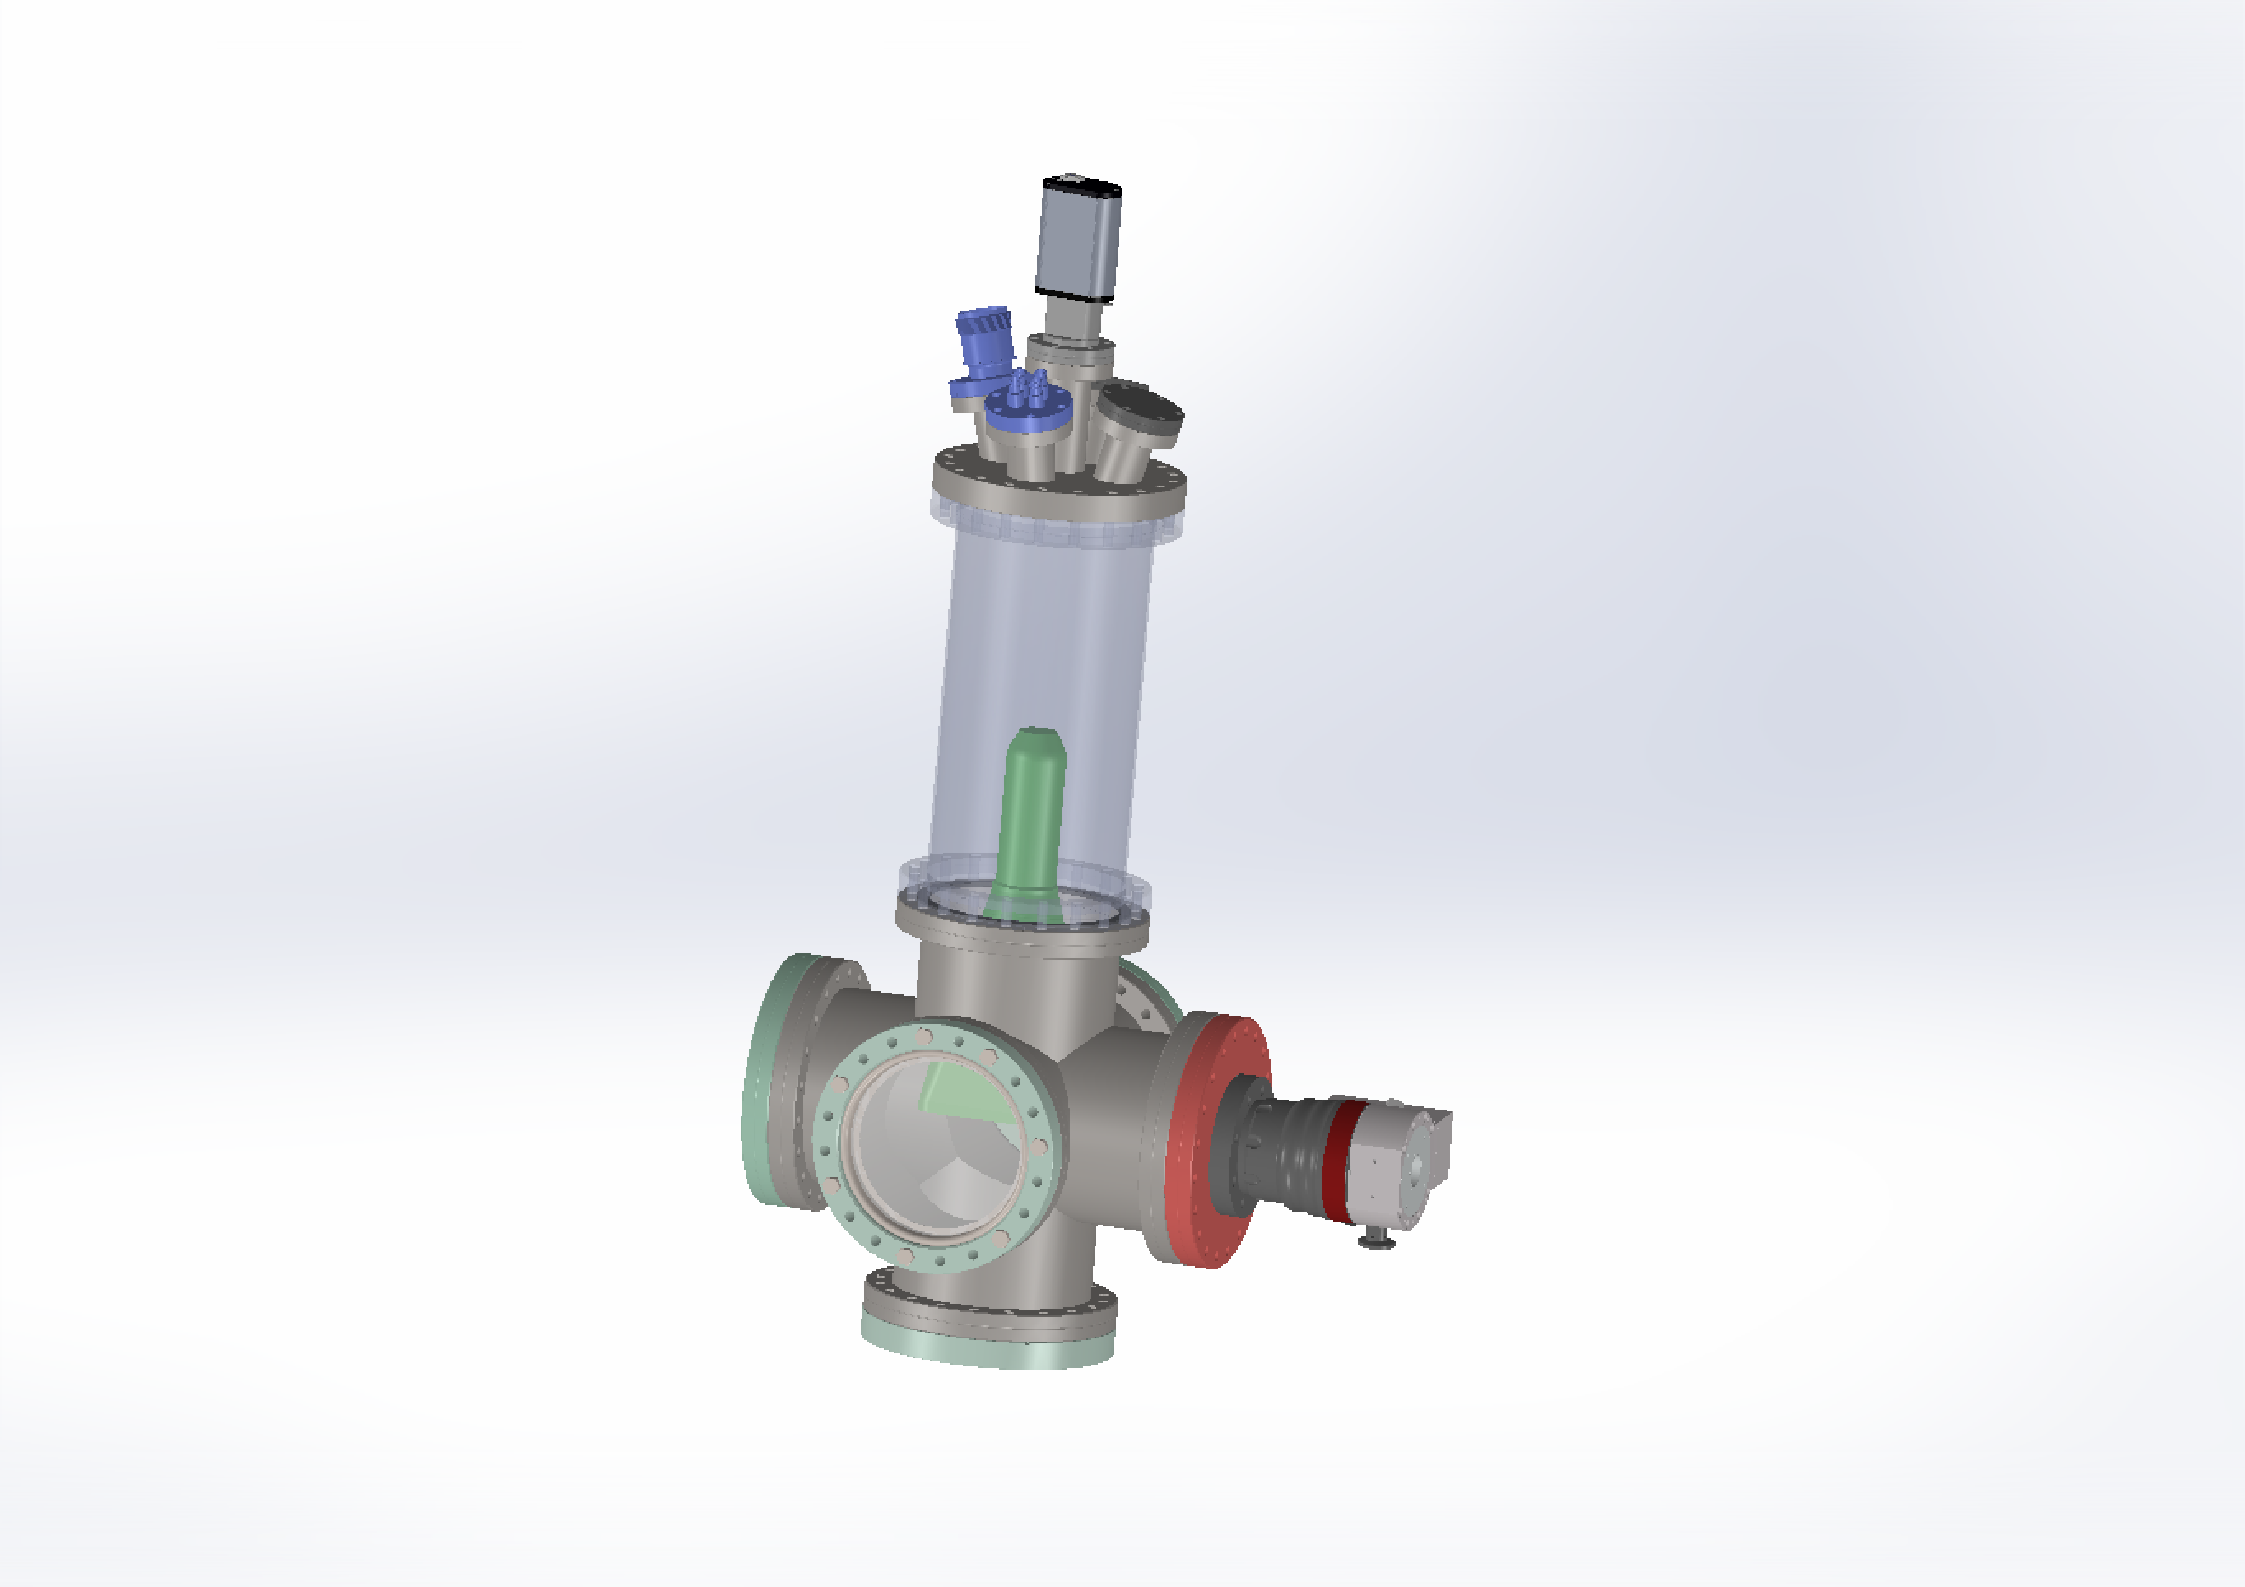
\includegraphics[width=0.9\textwidth]{./Chapters/vacuum-chamber/test_chamber} % taken from OneNote QuaK/Vacuum Setup/Test vacuum chamber
	
	\caption{3D rendering of test chamber.}
	\label{fig:3D rendering of test chamber}
\end{figure}
 
\subsection{CRT mounting mechanism}
\label{subsec:CRT mounting mechanism}

 Two M8 rods of length \todo{rod length?} were drilled into the cluster flange. On each, a L-piece was installed between two nuts and they were connected by a hose clamp. Two of these were used to secure the CRT inside the nipple facing the cross (\cref{fig:Image of CRT mounting mechanism}).
 

\begin{figure}[h]
	\centering
	
	\missingfigure[figwidth=0.9\textwidth]{Image of CRT mounting mechanism.}
	
	\caption{Image of CRT mounting mechanism.}
	\label{fig:Image of CRT mounting mechanism}
\end{figure}


\subsection{Leak test}
\label{subsec:Leak test}

Before inserting a CRT, a leak test was performed. First, the chamber was set to a pressure of \SI{e-5}{\milli\bar} after which the pump was turned off. The pressure was measured once a minute for a duration \SI{3}{\hour}. This is shown in \cref{fig:Leak rate of test chamber after turning off pump}.

\begin{figure}[ht]
	\centering
		
	\begin{tikzpicture}
		% !TeX encoding = UTF-8
% !TeX spellcheck = en_US
% !TeX root = ../../Thesis.tex

\begin{axis}[
	%name=zeemanShift,
	%grid=major,
	ymode = log,
	xlabel = time/\si{\minute},
	ylabel = pressure/\si{\milli\bar},
	%scaled ticks=false,
	%		every x tick scale label/.style={at={(xticklabel* cs:1.03,-0.3em)}, /pgfplots/near ticklabel align=outside, anchor=near xticklabel opposite, inner sep=0pt},
	%		xticklabel style={/pgf/number format/sci}, sci generic={mantissa sep=\cdot,exponent={10^{#1}}}},
	%yticklabel style={/pgf/number format/sci},
	xmin = 0,
	ymin = 1e-5,
	%extra tick style={grid=none}, 
	%width=0.7\textwidth,
	%legend style={at={(1.02, 0.5)}, anchor = west},
	%every axis plot/.append style={thick}
	]
	\addplot[mark=none, black] table [x=t, y=p, col sep=comma]{./Chapters/vacuum-chamber/leak_rate.csv};
\end{axis}
	\end{tikzpicture}
	
	\caption{Leak rate of test chamber after turning off pump.}
	\label{fig:Leak rate of test chamber after turning off pump}
\end{figure}


\section{Second iteration}
\label{sec:Second iteration}

At one point during experimentation, major changes were made to the chamber. Thanks to these, it was possible to reach a pressure of \SI{1.2e-7}{\milli\bar}.

\subsection{Changes}
\label{subsec:Changes}

First, every rubber gasket was changed to a copper one for a better seal, except at the cluster flange, since that spot will be opened and closed the most often. Each copper stranded cable inside was switched to a coaxial one and the mantle was connected to the chamber wall, which was set to ground. A Faraday cup was installed below the wobble stick, to accurately measure the beam current (further details in \todo{ref ch:Beam characterization}). The aluminum foil was extended to cover all four sides of the screen.

\subsection{Fastening}
\label{subsec:Fastening}

When attaching flanges, it is important to start with a low torque and to fasten opposite screws to prevent too much force on one side of the gasket. For M6 screws, the torque was incrementally set to \SIlist{6;10;15;20}{\newton\meter} and for M8 screws \SIlist{8;16;25}{\newton\meter}. After finishing every opposite screw pair at a set torque, the procedure was repeated twice before going to a higher torque. This was done in order guarantee a tight and even seal.

% !TeX encoding = UTF-8
% !TeX spellcheck = en_US
% !TeX root = ../../Thesis.tex

\chapter{Beam Characterization}
\label{ch:Beam Characterization}


\section{Aluminum foil}
\label{sec:Aluminum foil}

In \cref{fig:Front view of vacuum chamber} the inside of the vacuum chamber is shown. On one side of the phosphor screen, aluminum foil was attached to simulate the aquadag coating inside the cut CRT. The beam was deflected on the aluminum foil and the BNC output was connected to ground through an ammeter to measure the beam current. As shown in \cref{fig:Difference in filament voltage and beam current between an open and sealed CRT} there is nearly no difference in the filament voltage (and therefore heating power) between an opened and sealed CRT. The current going through the aluminum foil is much lower when compared to the current on pin g5 (which is connected to the aquadag coating) of a sealed device. One possible reason could be that electrons scatter. Therefore, a Faraday cup (see \cref{sec:Faraday cup}) was used.

\begin{figure}[h]
	\centering
	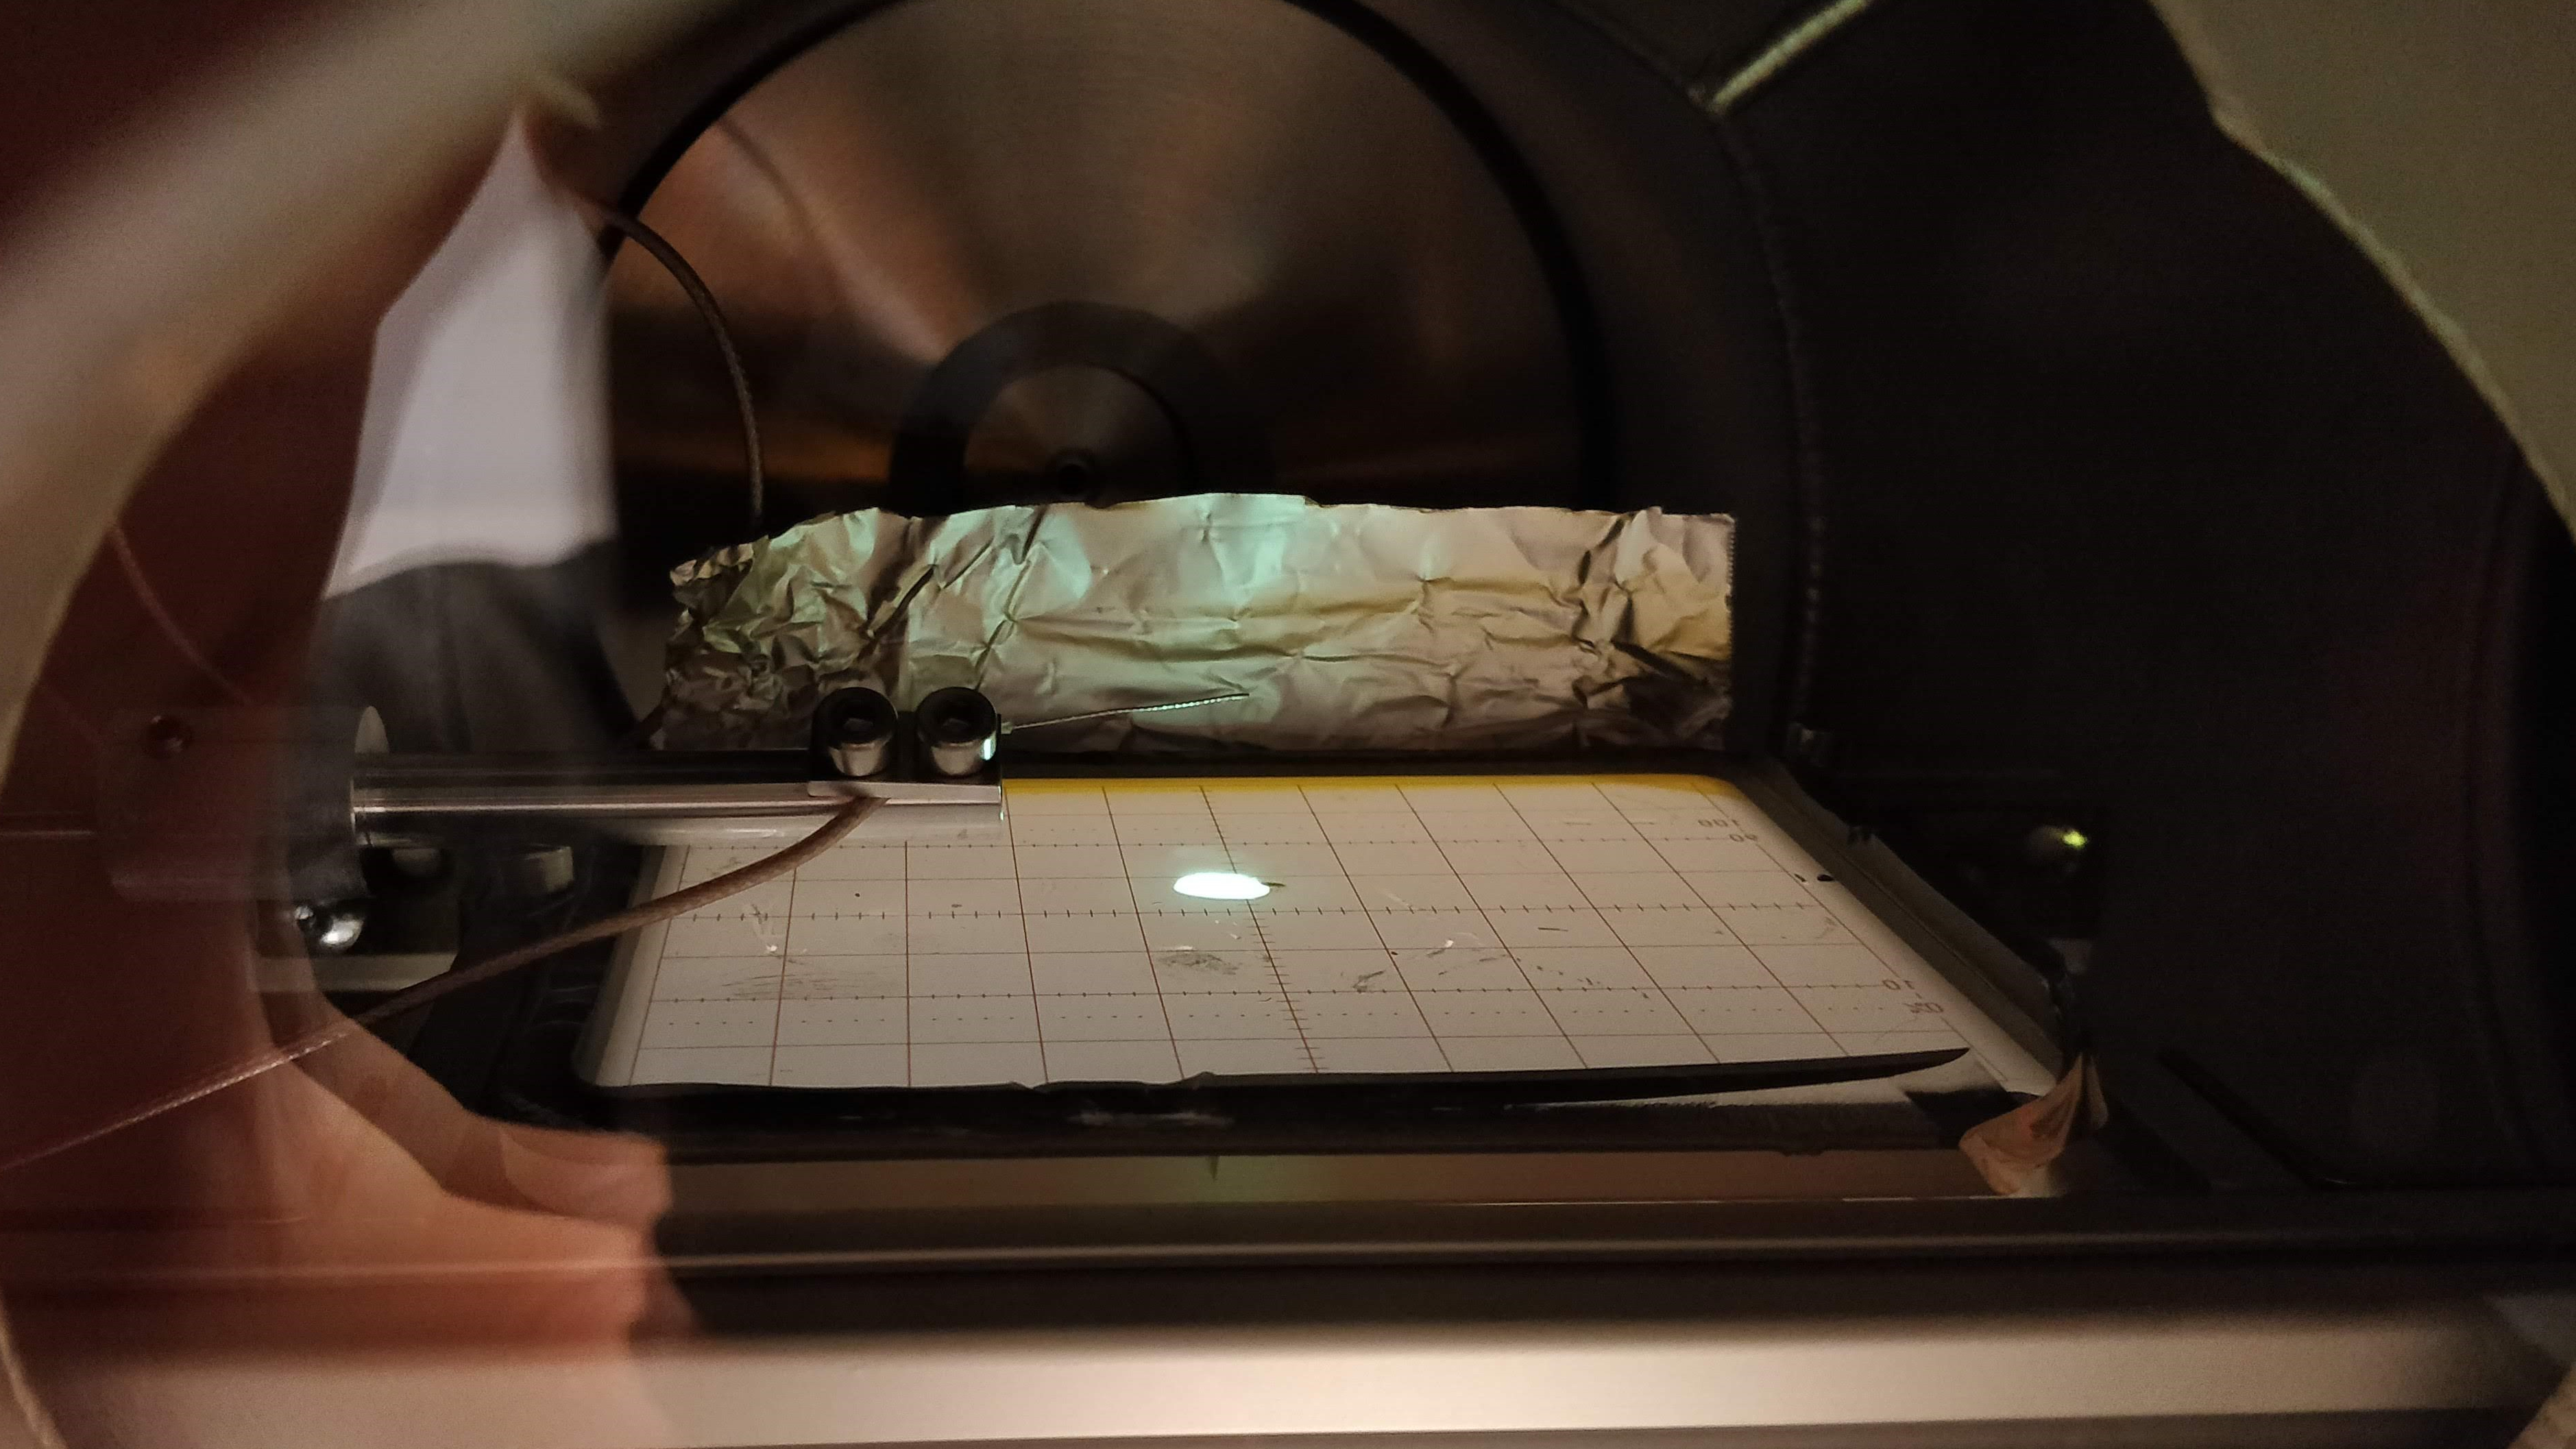
\includegraphics[width=0.9\textwidth]{./Chapters/beam-characterization/center_image}
	\caption{Front view of vacuum chamber.}
	\label{fig:Front view of vacuum chamber}
\end{figure}


\begin{figure}[ht]
	\centering
	% data OneNote 2019-10-22
	
	\begin{tikzpicture}
		% !TeX encoding = UTF-8
% !TeX spellcheck = en_US
% !TeX root = ../../Thesis.tex

\begin{groupplot}[
		group style={
			group size=2 by 1,
			horizontal sep=0.15\textwidth}, %0.1\textwidth},
		width=0.5\textwidth,
		height=0.5\textwidth]
	
	%1st plot
	\nextgroupplot[
		%title={},
		xlabel={filament current/\si{\milli\ampere}},
		ylabel={filament voltage/\si{\volt}},
	%	xmin=5, xmax=7.5,
	%	ymin=0, ymax=0.5,
		legend style={at={(0.05, 0.95)}, anchor={north west}},
		legend cell align={left}]
	
	\addplot+[
		black,
		only marks,
		mark=*,
		mark size=2pt,
		mark options={solid}]
	table [x=current_filament, y=voltage, col sep=comma]{./Chapters/beam-characterization/data_aluminum_foil_opened.csv};
	\addlegendentry{open}
	
	\addplot+[
		blue,
		only marks,
		mark=*,
		mark size=2pt,
		mark options={solid}]
	table [x=current_filament, y=voltage, col sep=comma]{./Chapters/beam-characterization/data_aluminum_foil_sealed.csv};
	\addlegendentry{sealed}
	

%	%2nd plot
	\nextgroupplot
	[
	%title={},
	xlabel={filament current/\si{\milli\ampere}},
	ylabel={beam current/\si{\micro\ampere}},
%	xmin=5, xmax=7.5,
	ymin=0, %ymax=0.5,
	legend style={at={(0.05, 0.95)}, anchor={north west}},
	legend cell align={left},
	]
	
	\addplot+[
		black,
		only marks,
		mark=*,
		mark size=2pt,
		mark options={solid}	]
	table [x=current_filament, y=current, col sep=comma]{./Chapters/beam-characterization/data_aluminum_foil_opened.csv};
	\addlegendentry{open}
	
	\addplot+[
		blue,
		only marks,
		mark=*,
		mark size=2pt,
		mark options={solid}]
	table [x=current_filament, y=current, col sep=comma]{./Chapters/beam-characterization/data_aluminum_foil_sealed.csv};
	\addlegendentry{sealed}
\end{groupplot}
	\end{tikzpicture}
	
	\caption{Difference in filament voltage and beam current between an open and sealed CRT.}
	\label{fig:Difference in filament voltage and beam current between an open and sealed CRT}
\end{figure}

\section{Faraday cup}
\label{sec:Faraday cup}

In order to accurately measure the full beam current, a Faraday cup was built. A schematic is shown in \cref{fig:Schematics of Faraday cup}. A copper tube was cut at an \ang{45} angle on one side and a Cu-sheet was soldered at the top and bottom. A small hole of around \SI{5}{\milli\meter} was drilled at the top and a coaxial cable was attached on the mantle which connects to a BNC feed through at the top of the chamber. The small opening and angled floor were added, in order to reduce electron loss through back scattering, as indicated by blue arrows in \cref{fig:Schematics of Faraday cup}. At the top surface a phosphor coating was applied, in order to make the beam visible. This made it easier to guide it into the opening hole.

\begin{figure}[h]
	\centering
	\begin{tikzpicture}
		% !TeX encoding = UTF-8
% !TeX spellcheck = en_US
% !TeX root = ../../Thesis.tex


%\draw [help lines] (-2, -2) grid (2, 5);


% cup
\draw (-0.3, 4) -- (-1, 4) -- (-1, -1) -- (1, 1) -- (1, 4) -- (0.3, 4);

% electron beam
\draw [blue] (0, 5) -- (0, 0);
\draw [blue, ->] (0, 0) -- (-1, -0.5);
\draw [blue, ->] (0, 0) -- (-1, 0.5);
\draw [blue, ->] (0, 0) -- (-1, 2);
\draw [blue, ->] (0, 0) -- (1, 2);
\node [right] at (1, 5) {\textcolor{blue}{e-beam}};

% 45 degree angle
\draw [dashed] (-1, -1) -- (2, -1);
\draw(-1+2, -1)arc [start angle=0,end angle=45, radius=2];
\node [right] at (1, 0) {\ang{45}};

% phosphor coating
\draw [fill=green] (-1, 4) rectangle (-0.3 , 4.1);
\draw [fill=green] (0.3, 4) rectangle (1, 4.1);
\node [right] at (1, 4.05) {\textcolor{green}{phosphor coating}};
	\end{tikzpicture}
	
	\caption{Schematics of Faraday cup.}
	\label{fig:Schematics of Faraday cup}
\end{figure}

With this improved setup, the beam current was measured again (\cref{fig:Beam current dependence on heater current}). It can be seen, that a current of over \SI{300}{\micro\ampere} was achieved, which is more than the necessary amount for the experiment. However, through this measurement it became evident that the current is not stable. A measurement on the next day under the same settings resulted in a current between \SIrange{50}{120}{\micro\ampere}.

\begin{figure}[h]
	\centering
	\begin{tikzpicture}
		% !TeX encoding = UTF-8
% !TeX spellcheck = en_US
% !TeX root = ../../Thesis.tex


	
%	%1st plot
%	\nextgroupplot[
%		%title={},
%		xlabel={filament current/\si{\milli\ampere}},
%		ylabel={filament voltage/\si{\volt}},
%	%	xmin=5, xmax=7.5,
%	%	ymin=0, ymax=0.5,
%		legend style={at={(0.05, 0.95)}, anchor={north west}},
%		legend cell align={left}]


\begin{axis}[
		%title={},
		xlabel={filament current/\si{\milli\ampere}},
		ylabel={beam current/\si{\micro\ampere}},
		%xmin=5, xmax=7.5,
		%ymin=0, ymax=0.5,
		%legend style={at={(0.05, 0.95)}, anchor={north west}},
		%legend cell align={left}]
	]
	\addplot[
		black,
		only marks,
		mark=*,
		mark size=2pt,
		mark options={solid},
	]
	table [x=current_filament, y=current_beam, col sep=comma]{./Chapters/beam-characterization/data_Faraday_cup.csv};
\end{axis}
	\end{tikzpicture}

	\caption{Beam current dependence on heater current.}
	\label{fig:Beam current dependence on heater current}
\end{figure}

\section{Deflection frequency}
\label{sec:Deflection frequency}

This section describes a few observations that were made when letting the electron beam interact with a short piece of wire which was mounted to the wobble stick. Originally, we hoped to be able to measure the beam waist, using the knife edge method, i.e. observing the current transported by the beam, while slowly moving a razor blade through the beam path. However the beam is bent, when it passes closely to a conductive part. Whenever, we moved our wire close to the beam, the visible spot on the Phosphorous screen below was distorted. This will probably complicate the measurement of the beam waist in the future. 
When the wire is connected to an oscilloscope, one can see a sharp increase in voltage, when it is moved into the beam. This can be used to see whether our deflection plates work properly and to test how fast we are able to deflect the beam. If the beam oscillates back and forth on a straight line and crosses the wire on the midway point, we should see a spike in voltage on the wire, which repeats with twice the frequency of the beam. If the wire is not on the midway point, the periods between consecutive spikes should sum up to the period of the beam's oscillation (see \cref{fig:spikes}). At low frequencies we have indeed observed this behavior. As the frequency is increased, the magnitude of the signal decreases. This is easily explained by the fact that the remain time close to the wire is inversely proportional to the frequency and the amplitude of beams deflection. To mitigate this, one should position the measurement wire at the maximum of the oscillation amplitude. If this is done, the induced amplitude becomes first order independent from the frequency. It was possible to see the spikes up to a frequency of \SI{100}{\kilo\hertz} before they where obscured by noise and some other periodical, but so far unexplained artifacts.
At high deflection frequencies, the wire may also pick up some signal form the capacitive charging and discharging of the deflection plates and the corresponding oscillating electromagnetic field.
In order to be able to see what happens at higher frequencies, a higher beam current and a smaller deflection amplitude would be beneficial.

% TODO: \usepackage{graphicx} required
\begin{figure}
	\centering
	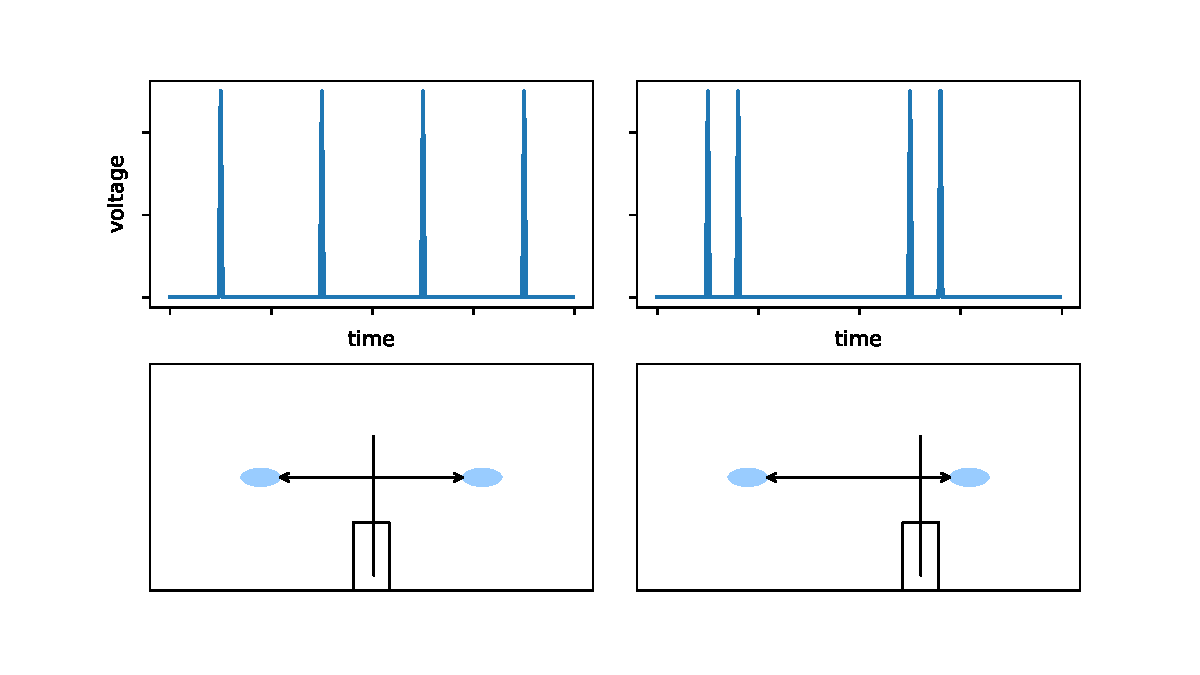
\includegraphics[width=0.8\linewidth]{Chapters/beam-characterization/Spikes}
	\caption{Observerd Voltage-spikes induced by an electron beam that was deflected periodically across a wire. (Arbitrary units)}
	\label{fig:spikes}
\end{figure}



%---backmatter-------------------------------------------------------------------
\backmatter
%---Appendix
\appendix
\renewcommand\thesection{\Alph{section}}			% lable sections with capital letters
%% !TeX encoding = UTF-8
% !TeX spellcheck = en_US
% !TeX root = ../../Thesis.tex
\chapter{Appendix}\label{chap:appendix}
\section{Appendix A}\label{sec:appendix_a}
\subsection{Source Code}\label{sec:source_code}
Here is some source code added with the lstlisting package. With \begin{verbatim}$£\vdots£$\end{verbatim} you can insert vertical dots to truncate code.
\begin{lstlisting}[basicstyle=\footnotesize, escapeinside={$£}{£$}]
/*++++++++++++++++++++++++++++++++++
+                   Awesome source code                    +
+                       TU Wien 2018                       +
+                      Thomas Weigner                      +
+                weigner.thomas@gmail.com                  +
+                         main.cpp                         +
+                         vers 3.4.1                       +
++++++++++++++++++++++++++++++++++*/

#include <header.h>
//---main program
int main(){
//---declare stuff and initialize things
$£\vdots£$
//------generating polynom for vertical transport
Poly polArray[5];           //Creating a polynom object array with the default constructor
double vMax = 2.0;          //maximal velocity
$£\vdots£$
\end{lstlisting}

\subsection{Matlab2Tikz}\label{sec:matlab2tikz}
Matlab to Tikz a is a very power full script to translate a Matlab figure into Tikz and Pgf code. After creating a file containing the code with this Matlab script one can do fine adjustments directly in the code. If you are not already using it you should go and check it out.
%---Index
\setindexpreamble{}							% expaletory text at the beginning of the index
\printthesisindex 							% list of todo in draft mode and index if index option is set
%---Lists
%\listoffigures								% print list of figures
%\listoftables								% print list of tables
%---Nomenclature
\renewcommand{\nomname}{List of Symbols}	% set nomenclature heading
\renewcommand{\nompreamble}{}				% set nomenclature preamble
\printnomencl{1ex}							% command for custom style nomenclature
%---Acknowledgement
%% !TeX encoding = UTF-8
% !TeX spellcheck = en_US
% !TeX root = ../../Thesis.tex
\begin{acknowledgements}\label{chap:acknowledgments}
Thanks to ...
\end{acknowledgements}

%---References-------------------------------------------------------------------
\begin{spacing}{0.9}						% adapt to change "density"
	\ifsetBibLaTeX
		\ifBibSections
			\printbibheading[heading=bibintoc, title={References}]
			\bibbysegment[heading=subbibliography]
		\else
			\printbibliography[heading=bibintoc, title={References}]
		\fi
	\fi
	\ifsetNatBib
	%---reference styles compatibel with natbib (choose one from the default folder or add one with relative path manually)
%		\bibliographystyle{naturemag} 		% nature magazine styled refernces
%		\bibliographystyle{newapa}			% improved American Psychological Assosiaction (apa) style
%		\bibliographystyle{apalike}			% similar to American Psychological Assosiaction (apa) styles
%		\bibliographystyle{abbrvnat}		% author abbreviations (natbib version of abbr)
%		\bibliographystyle{plainnat}		% numberical only (natbib version of plain)
		\bibliographystyle{unsrtnat}		% unsorted reference style (natbib version of unsrt)
	%---print bilbiography here
		\bibliography{./References/references.bib}
	\fi
\end{spacing}
%\include{./Chapters/Appendix/appendix_current_histroy_paper}
\end{document}
